%TC:ignore
\documentclass[12pt]{report}

\usepackage[utf8]{inputenc}
\usepackage[english]{babel}

\usepackage{array}
\usepackage{cmbright}
\usepackage{longtable}
\usepackage{tikz}
\usetikzlibrary{positioning, arrows.meta, shapes.geometric, shadows}
\usepackage{booktabs}
\usepackage{float}
\usepackage{setspace}
\usepackage{graphicx}
\usepackage{geometry}
\usepackage{fancyhdr}
\usepackage{listings}
\usepackage{afterpage}
\usepackage[numbers]{natbib}
\usepackage[bookmarks]{hyperref}
\geometry{left=1.25in, right=1in, top=1in, bottom=1in}

\newcommand\blankpage{%
    \null
    \thispagestyle{empty}%
    \addtocounter{page}{-1}%
    \newpage}

%%%%%%%%%%%%%%%%%%%%%%%%%%%%%%%%%%%%%%%%%%%%%%%%%%%%%%%%%%%%%%%%%%%%%%%%%%%%%%%%%%%%%%%%%%%%%%%%

\title{\textit{ReciproCast}: Enhancing Podcast Interactivity Through Conversational Avatars}
\author{Kieran Kasha}

\newcommand{\supervisor}{Tovi Grossman}

\usepackage{bera}% optional: just to have a nice mono-spaced font
\usepackage{xcolor}

\colorlet{punct}{red!60!black}
\definecolor{background}{HTML}{EEEEEE}
\definecolor{delim}{RGB}{20,105,176}
\colorlet{numb}{magenta!60!black}

\lstdefinelanguage{json}{
    basicstyle=\normalfont\ttfamily,
    numbers=left,
    numberstyle=\scriptsize,
    stepnumber=1,
    numbersep=8pt,
    showstringspaces=false,
    breaklines=true,
    frame=lines,
    backgroundcolor=\color{background},
    literate=
     *{0}{{{\color{numb}0}}}{1}
      {1}{{{\color{numb}1}}}{1}
      {2}{{{\color{numb}2}}}{1}
      {3}{{{\color{numb}3}}}{1}
      {4}{{{\color{numb}4}}}{1}
      {5}{{{\color{numb}5}}}{1}
      {6}{{{\color{numb}6}}}{1}
      {7}{{{\color{numb}7}}}{1}
      {8}{{{\color{numb}8}}}{1}
      {9}{{{\color{numb}9}}}{1}
      {:}{{{\color{punct}{:}}}}{1}
      {,}{{{\color{punct}{,}}}}{1}
      {\{}{{{\color{delim}{\{}}}}{1}
      {\}}{{{\color{delim}{\}}}}}{1}
      {[}{{{\color{delim}{[}}}}{1}
      {]}{{{\color{delim}{]}}}}{1},
}

\makeatletter
\renewcommand{\maketitle}{%
  \begin{titlepage}
    \onehalfspacing
    \begin{center}
      {\Large\textbf{\@title}\par}
      \vspace{\baselineskip}
      by\par
      {\large{\@author}\par}
      \vspace{\baselineskip}
      {\large Supervisor: \supervisor \\April 2024}
    \end{center}

    \vfill

    \begin{flushright}
    {\Huge\textbf{B.A.Sc. Thesis}}
    \end{flushright}
    
    \vspace{0.1\baselineskip}
    
    \begin{spacing}{0.4}
    \begin{flushright}
    \rule{3.25cm}{0.3pt}\\
    \rule{3.25cm}{0.3pt}\\
    \rule{3.25cm}{0.3pt}\\
    \rule{3.25cm}{0.3pt}
    \end{flushright}
    \vspace{-2\baselineskip}
    \rule{\textwidth}{0.3pt} 
    \rule{3.25cm}{0.3pt} \hspace{\textwidth} \rule{3.25cm}{0.3pt}\\
    \rule{3.25cm}{0.3pt} \hspace{\textwidth} \rule{3.25cm}{0.3pt}\\
    \rule{3.25cm}{0.3pt} \hspace{\textwidth} \rule{3.25cm}{0.3pt}\\
    \rule{3.25cm}{0.3pt} \hspace{\textwidth} \rule{3.25cm}{0.3pt}\\
    \rule{3.25cm}{0.3pt}\\
    \rule{3.25cm}{0.3pt}\\
    \rule{3.25cm}{0.3pt}\\
    \rule{3.25cm}{0.3pt}
    \vspace{2.5\baselineskip}
    \end{spacing}
    \begin{figure}[H]
        
\includegraphics[width=10.5cm]{logo.pdf}
    \end{figure}

  \end{titlepage}
}
\makeatother

\begin{document}
    \maketitle
    \afterpage{\blankpage} % Blank Flyleaf
    \clearpage
    
    \vspace*{\fill}
        \begin{center}
          \thispagestyle{empty}
          {\Large\textbf{\textit{ReciproCast}: Enhancing Podcast Interactivity Through Conversational Avatars}\par}
          \vspace{\baselineskip}
          by\par
          {\large{Kieran Kasha}\par}
          \vspace{\baselineskip}
          {\large Supervisor: \supervisor \\April 2024}
        \end{center}
    \vspace*{\fill}
    \clearpage
    
    \newenvironment{myfont}{\fontfamily{ntxtlf}\selectfont}{\par}
    %TC:endignore
    \begin{myfont}
        \pagenumbering{roman} % Roman numerals for preliminary pages
        %% Abstract
        \vspace*{\fill}
            \begin{center}
                \singlespacing
                \normalsize
                \begin{minipage}{0.8\textwidth}
                    \setlength{\parindent}{0pt}
                    \begin{center}
                        \Large\textbf{Abstract}
                    \end{center}
                    Podcasts have become increasingly popular; however, user interaction and consumption often remain limited to traditional audio player paradigms, relegated to little more than passive listening. Guided by our formative interviews, we present \textit{ReciproCast}. This novel system expands the interaction capacity of pre-recorded podcasts by allowing users to ask questions and receive tailored responses based on the original content. To achieve this, \textit{ReciproCast} employs large language models (LLMs) and text-to-speech generation to create "conversational avatars" that capture the personalities, knowledge, and voices of the speakers in the podcast episodes. Our user study shows that \textit{ReciproCast} transforms the formerly unidirectional podcast listening experience into a dynamic, conversational exchange, making it more engaging and personalized. The study results, a formal design space, and the presented future work opportunities identified in the paper lay the groundwork for future efforts to enhance interaction capabilities in speech-based content.
                \end{minipage}
            \end{center}
        \vspace*{\fill}
        \clearpage
        
        % Acknowledgements
        \vspace*{\fill}
            \begin{center}
                \singlespacing
                \normalsize
                \begin{minipage}{0.8\textwidth}
                    \setlength{\parindent}{0pt}
                    \begin{center}
                        \Large\textbf{Acknowledgements}
                    \end{center}
                        At the end of this undergraduate journey, I wish I could fill every page of this document with my gratitude for those who helped me through the late nights, who congratulated me on my successes, who stuck with me in my failures, and who guided me when I was lost in a sea of unfamiliarity. I wish I could name every friend, acquaintance, and colleague I've had the pleasure of interacting with. Firstly, I would like to thank Professor Tovi Grossman. Your success as a researcher and instructor is apparent in your commitment to your students, the quality of work the lab produces, and the passion you foster within it. To Bryan Wang, thank you for being such a supportive mentor, for listening to and engaging with my ideas, for giving me resources and support, and for constantly pushing me toward greater success. From the start, your supportiveness led me to seek out a problem I was genuinely interested in and thought was worth solving. Your kindness, generosity, time, and plethora of experience have been instrumental to this project and my undergraduate experience. To Sangho Suh, thank you for all your help this past year. Your insights and ideas have always been beneficial to me in terms of helping me learn and beneficial to the project and its outcomes. To the other members of the Dynamic Graphics Project, thank you for sharing your space, projects, questions, and suggestions. Thank you, especially to Stephen, for letting me steal his desk! I also want to extend my gratitude to all those who agreed to participate in the formative interviews and user studies. Your perspectives truly formed the foundations of this project. I would not be here without my loving family. To my parents, Kevin and Kim, I cannot begin to thank you enough for never letting me give up on my dreams and supporting me during every step towards them. To my sister, Kaitlyn, I want you to know how much I've always looked up to you and how that has always guided me towards betterment. Lastly, to my immaculately majestic girlfriend, Taylor, thank you for always helping me find the strength to push through it all. I hope you all can see yourselves in this work as much as I see you.
                \end{minipage}
            \end{center}
        \vspace*{\fill}
        \clearpage
        
        % Table of Contents
        \tableofcontents
        \clearpage
        
        \clearpage
        
        \addcontentsline{toc}{chapter}{\listfigurename}
        \listoffigures
        \clearpage
        
        \addcontentsline{toc}{chapter}{\listtablename}
        \listoftables
        \clearpage
        
        \pagenumbering{arabic} % Arabic numerals for main pages

        \onehalfspacing
        
        % Body of the Thesis
        % ######################## Introduction ##########################
        \chapter{Introduction}
        The contemporary digital era has ushered in innovative entertainment mediums that vie for consumers' attention and leisure time as a primary currency. Among these, podcasts have achieved near-ubiquity over the past decade. This popularity has attracted a global audience of over 450 million listeners and propelled the podcast industry to produce over 3 million podcasts, amassing an impressive 18.52 billion USD in 2022 revenue \citep{CramerFlood2020}\citep{ListenNotes2023}\citep{GrandViewResearch2023}. Despite the growth of the medium, the interface between the podcast, the listener, and hosting platforms remains less explored. Podcasts, inherently auditory and pre-produced, present challenges in offering real-time interactivity. Currently, interaction in the podcast domain mainly involves listeners passively consuming podcast content (Interaction Type B) and simply manipulating its playback (Interaction Type C), as depicted in Figure \ref{fig:interaction}. A clear gap, indicated by arrow A in Figure \ref{fig:interaction}, represents a more multidirectional and meaningful interaction between listeners and the podcast media. Defining what this type of interactivity should look like in the podcast space and designing methods that enable novel user engagement remains largely untouched in academic research. Therefore, the goals of this research are fourfold: to conduct formative interviews with podcast consumers and creators to gauge their interest in and preferences for greater interactivity, to utilize these findings to create a formal design space of viable features that enhance podcast interactivity, to construct a prototype of a platform that implements features from the design space that best bridge the interactivity gap, and to validate this prototype in a user study.\\
        \begin{figure}[H]
        \centering
          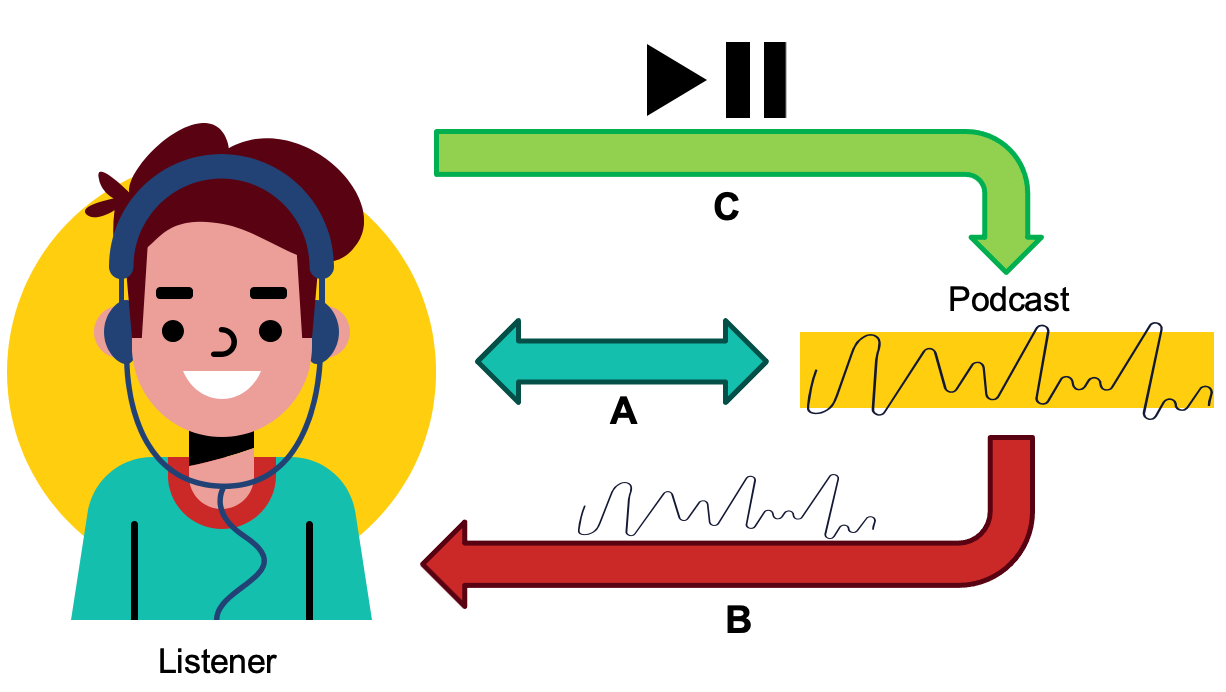
\includegraphics[width=1\textwidth]{figures/interaction.png}
          \caption{Types of podcast interactivity where B and C represent traditional passive listening and playback control, respectively, and A represents a novel type of reciprocal interaction.}
          \label{fig:interaction}
        \end{figure}
        \indent The formative interviews revealed that podcast listeners and creators alike are dissatisfied with the current status quo of passive and detached interaction. Currently, podcasts are similar to traditional classroom learning, where a single creator or teacher disseminates educational material to multiple listeners or learners. Studies have overwhelmingly shown that traditional classroom learning via passive listening is not nearly as engaging as one-on-one instruction \citep{WoodTanner2012}\citep{Hanley2018}\citep{WangChristensen2020}. The perspectives of interviewed listeners supported this analogy well. Upon initial survey, 71.4\% of the listeners believed that greater interactivity would provide an enhancement over their current experience. Creators were even more interested, with 87.5\% of them wishing for greater interactivity. These results are summarized in Figure \ref{fig:formative1}. Given these findings, we have developed a design space that illustrates various opportunities to expand the interactive capabilities of podcasts. Within this design space, we specifically focus on a feature that emerged as the most popular in the formative interviews: the ability for listeners to converse with the people involved in the podcast episode to ask questions about content and discuss their perspectives.\\
        \begin{figure}[H]
        \centering
          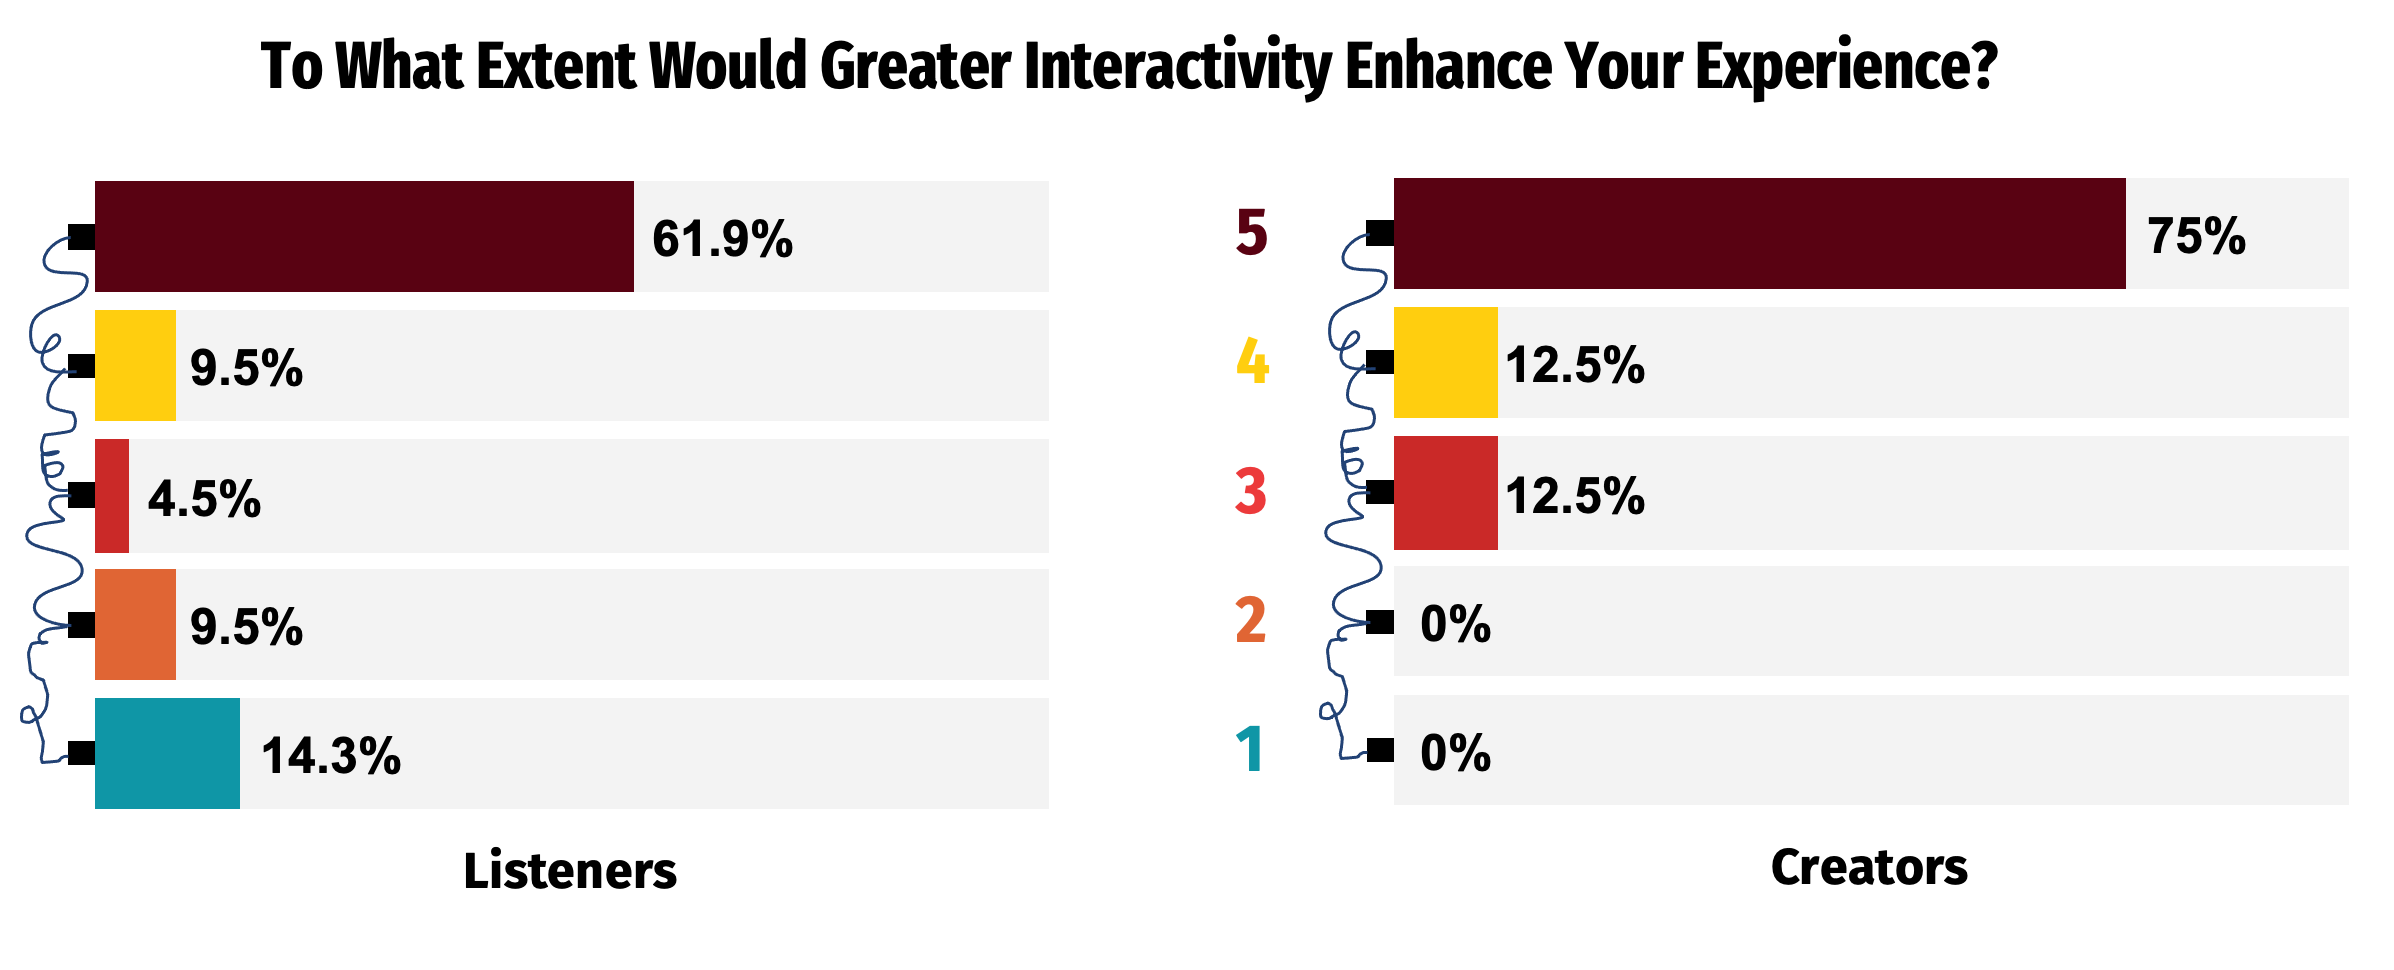
\includegraphics[width=1\textwidth]{figures/formative1.png}
          \caption{Formative interview survey results showing the interest in greater interactivity in the podcast space for creators and listeners.}
          \label{fig:formative1}
        \end{figure}
        \indent Therefore, we present \textit{ReciproCast}, a system that enables a novel and reciprocal interaction between the podcast and the listener. \textit{ReciproCast} is built upon what we call "conversational avatars." These conversational avatars leverage Large Language Models (LLMs), specifically GPT-4 Turbo. LLMs were chosen because they have successfully engaged users through conversational interfaces \citep{OpenAI2023GPT4}. After loading in a podcast episode, the system utilizes the podcast transcript and audio snippets of each person speaking to generate an avatar of them, representing an approximation of their thoughts and opinions while using a clone of their voice. \textit{ReciproCast} facilitates different conversational modes dynamically from the prompt alone via a \texttt{ConversationManager} class. This manager again uses LLMs to determine if the prompt should go to a particular conversational avatar or if a multi-avatar discussion should occur, allowing for a more natural conversational experience that doesn’t require the user to request a certain conversation type explicitly. Lastly, \textit{ReciproCast} includes a generic assistant conversational avatar named AIden, who is meant to provide more general knowledge and may intervene if responding to a prompt directed to a human-based avatar may cause harm to whomever that avatar represents.
        
        \indent Finally, the user study validated that \textit{ReciproCast} is a promising tool for podcast interactivity. For listeners, \textit{ReciproCast} allows users to engage directly with the podcast material, getting answers and clarifications to podcast content in real time. Listeners expressed the feeling of being allowed into the recording room and invited to be part of the conversation, a novel experience that enhanced their listening experience. For creators, \textit{ReciproCast} alleviates the need to respond to every listener's inquiries and presents potentially new avenues of community cohesion and monetization. Thus, the user study provided insight into how this project may be expanded into other regions of the design space to better benefit listeners and creators within the podcast space and potentially in other content-centric mediums.
        
        \indent Through the development of \textit{ReciproCast}, this thesis addresses a significant gap in the current podcasting experience and pioneers a model for interactive media that could influence future content delivery across various platforms. By integrating advanced LLMs and user-centred design practices, \textit{ReciproCast} promises to transform podcast listening from a passive activity into an engaging, interactive experience \citep{Hochheiser2017ExperimentalDesign}. The validation through user studies confirms its potential, setting the stage for further exploration and development in this emerging field.\\

        % ######################## Related Work ##########################
        \chapter{Related Work}
        In the evolving digital media landscape, interactivity has emerged as a critical factor in enhancing user engagement and personalizing content across various platforms. Interactivity is the proclivity of a system to support, adapt, and provide feedback based on a variety of user inputs \citep{Sundar2010Designing}. Interactivity forms a centrepiece of human-computer interaction (HCI) due to the recognition that interactive elements capture users' attention and significantly enrich their experience by making it more immersive and responsive \citep{Sundar2010Designing}. The concept of interactivity in media interfaces has been extensively studied, with researchers identifying it as a pivotal element influencing user engagement through various psychological mechanisms. Sundar \textit{et al.} \citep{Sundar2010Designing} describe how interactivity exists in different loci of communication: the source or creator of the content, the medium of delivery, and the message or content itself. Thus, interactivity arises in systems that allow users to meaningfully alter the source, medium, or message of the media they consume.
        
        \indent This section will review the existing literature and projects in digital audio interactivity, mainly focusing on podcasts, to highlight the current state, limitations, and significant opportunities for innovation in this space. In doing so, we will underline the necessity of exploring new interactive technologies, like Large Language Models (LLMs), to bridge the identified gaps and push the boundaries of what interactive digital audio content can achieve.
        
        \section{Advancements Into Audio Interactivity}
        \indent Historically, interactivity in audio content began with simple manipulations like choosing tracks or adjusting volume and playback, similar to the current state of podcast interaction as shown in \ref{fig:interaction}. However, transforming passive audio experiences into interactive narratives is not entirely new. For instance, Furini \citep{Furini2007Beyond} proposed an interactive audiobook system where listeners could actively shape the storyline through pre-defined choices at crucial narrative points. This system comprises several components: a Script Manager, a Scene Manager, an Interaction Manager, and an enhanced Audiobook Player. These components collaborate to manage the audiobook's script by dividing the story into multiple audio scenes and defining possible scene transitions that depend on user interactions. Furini claims that these interactions allow the user to transition from passive listeners to active participants, capable of directing the story's outcome \citep{Furini2007Beyond}. However, the quality and quantity of these choices are inflexible and limited to those accounted for by audiobook creators. The issue with this is that it significantly increases the creative overhead for creators and the attention they have to place on continuity, lest the choices become incongruent to the outcome or awkward to the narrative in general. The paper presents other limitations to such a system, including recognizing that while this type of interaction is novel within the medium, it is imperative to determine if user interest exists \citep{Furini2007Beyond}.
        
        \indent Moreover, researchers Piñeiro-Otero and Pedrero-Esteban \citep{Piñeiro-Otero2022Audio} have argued that we currently live in a "renaissance of digital audio," highlighting significant transformations in how audio content is consumed and produced in the digital age. The proliferation of podcasts characterizes this renaissance, the surge in streaming music platforms, and the increasing role of audiobooks and smart speakers, fundamentally shifting the audio landscape from traditional broadcasting to a more diversified digital medium. These changes have brought about a convergence of technologies and formats, enabling personalized and on-demand audio experiences that cater to individual preferences and behaviours through advanced recommendation algorithms \citep{Piñeiro-Otero2022Audio}. However, despite these advancements, the interactivity in digital audio, particularly in non-live podcasts, still heavily focuses on the medium of delivery as the primary locus of interaction, often neglecting the content as an interactive focus that allows for greater user engagement \citep{Sundar2010Designing}. As we delve into the current state of podcast interactivity, it becomes clear that there is a significant opportunity to further integrate listener feedback into the content direction in real time, enhancing the depth and richness of user experiences in the digital audio space.
        
        \section{The Current State of Podcast Interactivity}
        \indent The current landscape of podcast interactivity is characterized by its dual focus on both the delivery technology and the modes of listener engagement. While podcasts inherently allow for asynchronous consumption, their interactivity is confined to listener control over playback features such as pause, rewind, and fast-forward. Traditionally, podcasts are passively consumed; the download or stream is the primary interaction point. Studies, such as those by Burns \citep{Burns2010The}, have highlighted that podcasts still essentially function as closed systems with minimal listener input on the consumed content. Burns describes the process as a one-way interaction where content is pushed to listeners who have little opportunity to influence or interact with the content beyond choosing to play or skip it \citep{Burns2010The}. This model underscores a significant limitation in the evolution of podcast interactivity, emphasizing the need for platforms that can incorporate more dynamic and multidirectional forms of engagement.
        
        \subsection{Podcast Engagement Factors}
        \indent Building on the landscape outlined by Burns \citep{Burns2010The}, García-Marín \citep{GarciaMarin2020} delves deeper into the factors that could potentially invigorate listener engagement. These engagement factors fall under three main categories: medium-centred, user-centred, and podcaster-centred. \\
        \indent The medium-centred category includes platform-specific technological biases and the asynchronous nature of podcasts, which influence when and how content is consumed. The paper highlights a limitation that this asynchronous nature can lead to less timely interactions between listeners and podcast creators \citep{GarciaMarin2020}. Some podcast platforms allow for the live broadcasting of episodes that help to mitigate this problem. Still, there is no clearly defined solution for purely pre-produced podcast episodes, which constitute the majority of podcasts consumed \citep{GrandViewResearch2023}. The study further indicates that the design of podcast apps often "relegates the user to an exclusively passive role" by withholding options for real-time feedback, like leaving comments or manipulating content to user preference, echoing Burns' observations of podcasts as largely one-way systems \citep{GarciaMarin2020}\citep{Burns2010The}. 
        
        \indent In the user-centred category, factors like how much listener participation is encouraged by the podcaster or platform, the environment or situation in which users are consuming podcasts, and the number of podcasts the user subscribes to affect how engaged listeners might be \citep{GarciaMarin2020}. Importantly, it suggests that even though the digital nature of podcasts should theoretically facilitate greater interactivity, actual listener engagement is frequently limited by the contexts in which podcasts are consumed—often during activities that preclude active participation (e.g., driving, working) \citep{GarciaMarin2020}. This reality points to the underutilized potential of podcasts to foster more meaningful engagement.
        
        \indent Lastly, the podcaster-centred factors focus on podcast creators' skills, attitudes, and tone, which can significantly influence engagement levels. The paper argues that podcasters who effectively use their platform to invite listener interaction can enhance the participatory experience. However, how platforms limit direct interaction between podcasters and their audience remains a significant barrier to transforming podcasting into a fully interactive experience \citep{GarciaMarin2020}.
        
        \indent These factors reveal critical areas of improvement to overcome the limitations of the current podcast space. By addressing these factors, there is potential to enhance the interactivity of podcasts beyond mere content consumption, encouraging a more dynamic and participatory listener experience. This evolution would require technological advancements in podcast platforms and a shift in how podcasters and listeners perceive and engage with podcast content.\\
        \subsection{Interactive Projects in the Podcast Space}
        \indent Some projects, both proprietary and research-focused, have attempted to further the podcast medium by engaging with these factors. One example is \textit{Crosscast}, which enhances podcasts with visuals, adding a layer of medium-centered interactivity that enriches the user experience by engaging multiple senses via multi-media integration \citep{Crosscast}. Similarly, \textit{Podcast.ai} pushes the boundaries of user-centred interactivity by allowing users to submit ideas for weekly AI-generated podcast discussions featuring historical figures, offering listeners a unique blend of education and engagement \citep{PodcastAI2023}. Additionally, \textit{Podreels} represents an intersection of user-centred and podcaster-centred interactivity by enabling human-AI co-creation of video podcast teasers \citep{wang2024podreels}. This collaboration extends the podcasting experience beyond mere consumption, allowing creators to leverage AI to enhance promotional content and engage listeners in novel ways. Although each of these ventures contributes to expanding podcast interactivity, they remain enhancements to the existing structure rather than transforming it.
        
        \indent Continuing from this analysis, the concept of intimacy, as explored in podcast literature, suggests an inherent potential for personalized and conversational interactivity \citep{Berg2023Analysing}. Listening experiences that foster a perceived closeness between the listener and the podcast host cultivate intimacy, which could be the foundation for interactive experiences. For example, the conversational nature of podcasts can evoke a sense of dialogue despite the listener's role being traditionally passive. Research conducted by Berg \citep{Berg2023Analysing} suggests that the conversational nature of podcasts can evoke a sense of dialogue despite the listener's role being traditionally passive. This intimacy, as Berg explores, can significantly enhance listener engagement by deepening the connection between the podcast and its audience through a sense of personal interaction and belonging. However, despite these inherent capabilities of podcasting to forge intimate experiences, the actual integration of these interactive features into the podcasting format varies widely. Many podcasts do not fully exploit the potential for interactive engagement, often hindered by technological limitations, the inherent structure of podcasts, or the content strategies employed by creators. Thus, while the medium offers substantial opportunities for creating intimate and engaging listener experiences, the full potential of these interactions is not always realized in the current podcasting landscape. This inconsistency highlights a gap in leveraging intimacy as a strategic tool for enhancing podcast listeners' engagement and interactivity.
        
        \section{The Role of LLMs in Podcast Interactivity}
        \indent The conversational capacities of LLMs, trained to engage in natural, human-like dialogue, could offer new pathways for listeners to interact with podcast content, building upon this idea of intimacy to break down the traditional barriers of asynchrony. However, while LLMs could help form the backbone of interactive podcast platforms, there is a severe lack of research into how LLMs can be used within podcast media. LLMs have shown immense success in summarization and have become the ubiquitous backbone of state-of-the-art, flexible chat-bots \citep{OpenAI2023GPT4}. Nothing stops LLMs from transforming the podcast experience as they have the educational landscape; however, the only major research project that has attempted to do so was quite limited in scope and framing \citep{Laban2022NewsPod}.
        
        \indent NewsPod is an initiative that automatically generates news-focused podcasts in a question-and-answer format \citep{Laban2022NewsPod}. NewsPod carved out a niche by structuring each podcast segment around a current event using a news article as a source and employing two distinct text-to-speech voices for the 'questioner' and 'answerer,' thus facilitating a conversational flow \citep{Laban2022NewsPod}. NewsPod also allowed listeners to pose questions and receive automated responses \citep{Laban2022NewsPod}. The researchers conducted a user study showing demand for such a system, with 85\% of participants electing to ask at least one question \citep{Laban2022NewsPod}. The project leveraged neural networks such as WaveNet and Tacotron for text-to-speech, employed an LLM called RoBERTa for extractive question answering and utilized a neural network called PEGASUS for creating summaries for the beginning of each generated episode \citep{Laban2022NewsPod}.
        
        \indent While NewsPod was the first paper to target the podcast experience with machine learning technology in this manner, the project has severe limitations. First, NewsPod relies on extractive models for question-and-answer generation. If the input news articles do not explicitly state the answer, no answer could be extracted, highlighting a lack of depth in the interaction \citep{Laban2022NewsPod}. If the answer is not located within the text, users were provided with a generic response that stated an answer could not be provided before the podcast audio resumed. Third, the project's generative nature and specific model used for creating the summaries raised concerns over factual accuracy, with the model having the propensity to develop factually incorrect, potentially misleading, or confusing information. Fourth, while users were generally satisfied with the generated answers for the question-and-answer podcast audio, 76\% of participants stated that the answers they received were irrelevant or confusing \citep{Laban2022NewsPod}. Fifth, 15\% of participants were dissatisfied with the quality of the synthesized speech \citep{Laban2022NewsPod}. Furthermore, users could only submit questions by typing them in, which may not be viable for users of varying abilities or in different listening environments. Lastly, the researchers employed participants from Amazon Mechanical Turk for the user study. This crowdsourcing service allows researchers to find anonymous participants to perform paid tasks. Thus, no effort was made to verify that the participants were podcast consumers, and the fact that they were compensated for engaging with the prototype must be considered when the paper asserts that interaction taking place corresponded with authentic engagement or demand \citep{Laban2022NewsPod}.
        
        \indent Thus, this research aims to transcend the limitations observed in NewsPod by incorporating a more sophisticated approach to interactivity within podcasts. Where NewsPod's question-and-answer system was purely extractive and limited by the source material, this project integrates conversational and 'open-domain' question-answering capabilities, allowing for a richer, more dynamic interaction that can accommodate a broader range of listener inquiries \citep{Laban2022NewsPod}. Moreover, since the publication of NewsPod, the state-of-the-art of LLM technology has only advanced with models like GPT-4 \citep{OpenAI2023GPT4}. Thus, the quality of answers will be a primary area of improvement.
        
        \section{Summary of Research Gaps}
        \indent The reviewed literature reveals several key gaps in podcast interactivity that can direct future research. These gaps include: 

        \begin{enumerate}
            \item \textbf{Limited Dynamic Interaction}: Existing podcast platforms predominantly limit interactivity to basic playback controls. There is a significant opportunity to expand beyond these features to include more dynamic, real-time interactions between listeners and podcast content.
            \item \textbf{Inflexible Content Manipulation}: Current interactive audio systems, like the interactive audiobook model discussed, offer limited and predefined user choices, which do not allow listeners to shape the narrative dynamically or contribute content creatively.
            \item \textbf{Engagement in Non-Live Formats}: Most podcasts are asynchronously consumed, challenging the incorporation of real-time listener feedback and interaction. This limitation leads to predominantly passive consumption, where the listener's role is minimally influential. This problem is especially apparent when commenting or other feedback forms are unavailable on the platform.
            \item \textbf{Need for Enhanced Listener Experience}: A gap exists in creating a more engaging listener experience that leverages podcasts' intimacy and conversational nature. Current methods do not fully utilize the potential for podcasts to offer personalized, conversational interactivity that mirrors real dialogue.
            \item \textbf{Technological Underutilization}: Despite advancements in digital audio technology, the potential for integrating sophisticated interactive tools in podcasts has been underexplored. This opportunity includes leveraging AI and LLMs to enhance content personalization and interaction. Research is scarce regarding how LLMs could be specifically utilized within the podcast medium to enhance interactivity. Existing studies like NewsPod have shown the potential but highlighted limitations in scope, interaction depth, and user satisfaction.
        \end{enumerate}
        
        \indent Building on these identified research gaps, the next section will explore the design and implementation of formative interviews with podcast listeners and creators. These interviews aim to gather insights on expectations, preferences, and perceived barriers to podcast interactivity. The insights from these interviews will be crucial in proposing a design space for podcast interactivity that addresses the current limitations and optimally utilizes emerging technologies.
        \clearpage

        \chapter{Design Formulation}
        This section outlines the steps taken to establish what type of interactive design would satisfy users' needs in the podcast space. To do this, we conducted a set of formative interviews. The insights from these interviews led to creating a formal design space that indicates how different design ideas may fit within user expectations and needs. The design goals relevant to this project are firmly established from this design space, allowing us to proceed with the implementation.
        
        \section{Formative Interviews}
        The formative interviews took place both in person and over Zoom. Overall, 21 people responded to our initial survey. From this, we scheduled 12 interviews: 8 with podcast consumers and 4 with podcast creators. The initial survey included questions tailored towards listeners and creators separately; creators were also encouraged to respond to the listener questions. First, demographic information was collected about the respondents to ensure that a diverse range of individuals would provide their insights. Figure \ref{fig:demographics} shows the results of this portion of the survey. 
        \begin{figure}[H]
        \centering
          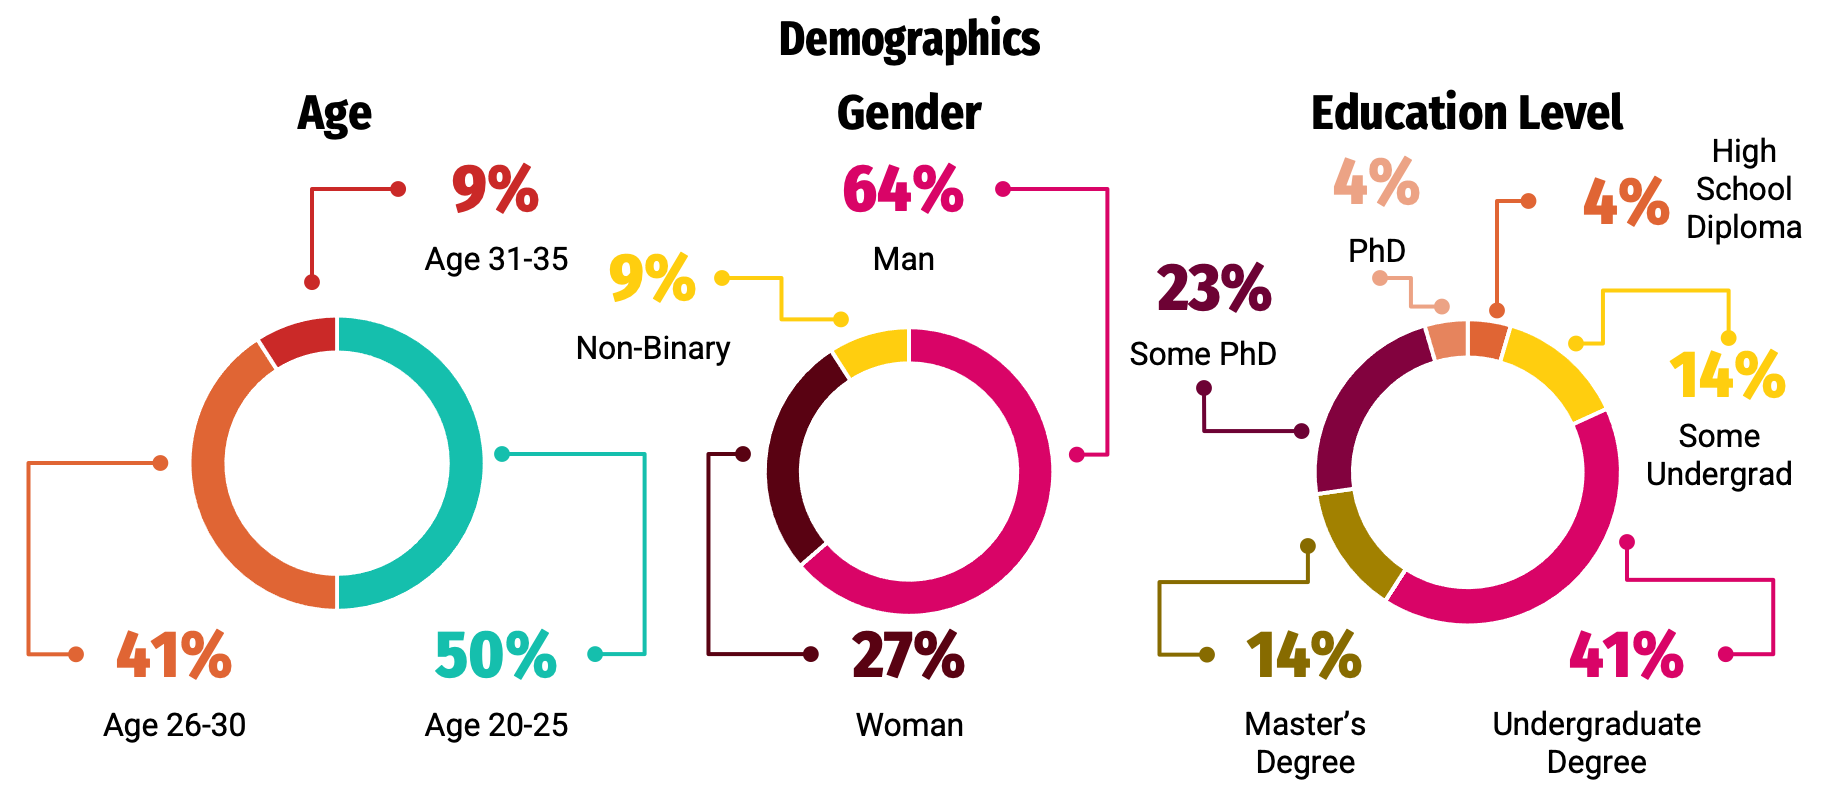
\includegraphics[width=1\textwidth]{figures/formative_demographics.png}
          \caption{Demographic information collected in the formative interview survey, including the age, gender identity, and education level of participants.}
          \label{fig:demographics}
        \end{figure}
        \indent The part of the survey meant for creators contained questions about years of experience, the genre of the podcasts they create, the platforms and programs they use during the creation process, and strengths and weaknesses of the current methods of podcast creation. The listener portion included questions about the frequency of podcast consumption and how long the listener has been consuming podcasts, the platforms they use to listen to podcasts, the genres of podcasts they listen to, the environment in which they listen to podcasts, their preliminary likes and dislikes about the current status quo of podcast consumption and their reasons for listening to podcasts. Figure \ref{fig:consumption} shows that the most common environment for listening to podcasts was at home, where 95\% of respondents identified it as one of the places they listen to podcasts. The other environments, such as doing chores, commuting, or being at work, each provide different constraints to what type of interaction is possible. For instance, it may not be good to require the user to speak out loud if they are commuting, but it may not be possible to use their hands freely while doing chores. Finally, creators and listeners agreed podcast interactivity would improve their experience, as shown in Figure \ref{fig:formative1}. Following this, they were asked to imagine what features they would like to see in 5-10 years, given unlimited technological advancement. These responses would form the foundation for the interview discussions. Interestingly, while some listeners disagreed with the statement, as seen in Figure \ref{fig:formative1}, their interviews were still quite insightful into methods for incorporating interactivity in podcasts. See Appendix \ref{app:A} for more detailed results from the survey.
        
        \begin{figure}[H]
        \centering
          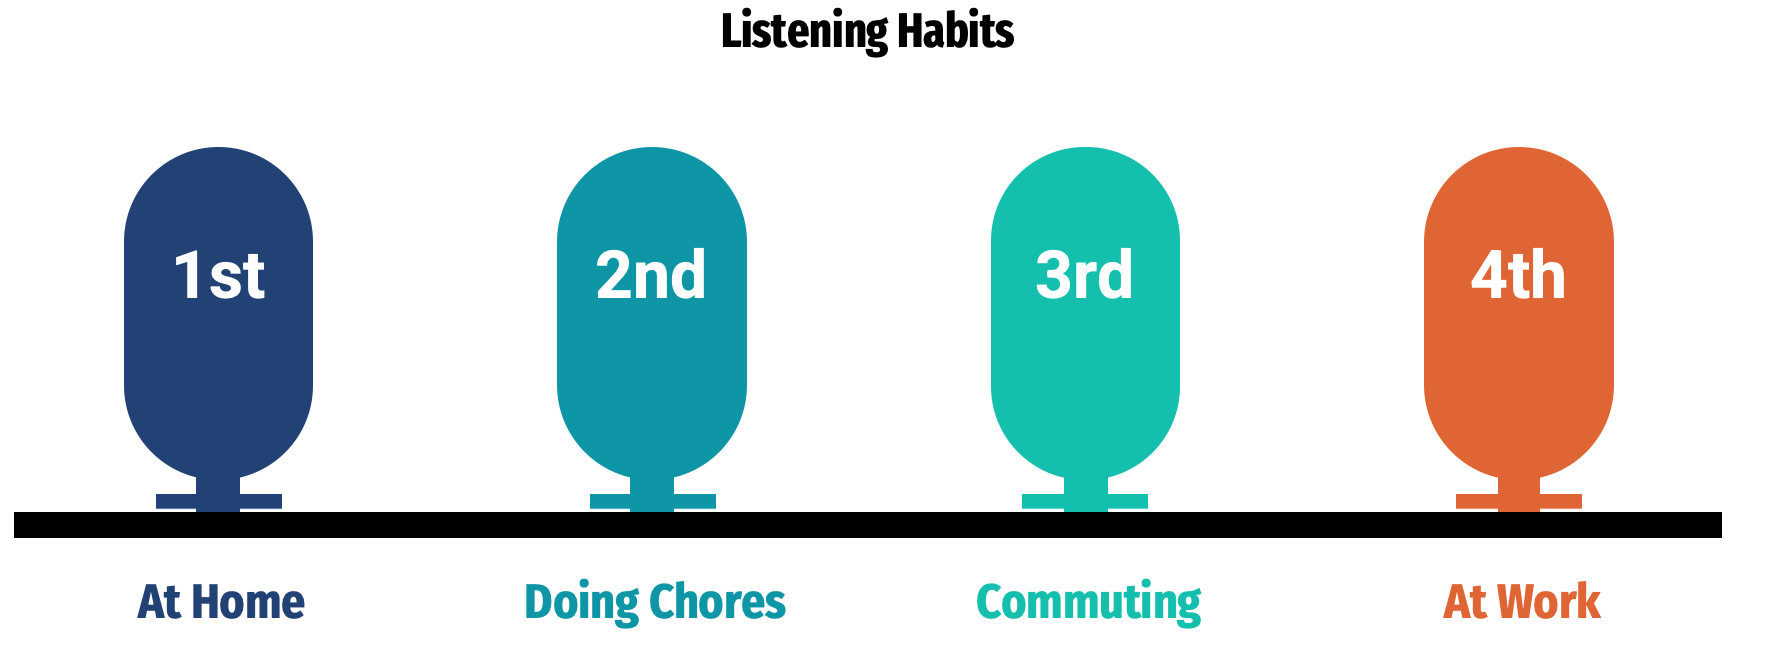
\includegraphics[width=1\textwidth]{figures/consumption_habits.png}
          \caption{A ranking of the top four environments in which the respondents of the formative interview survey consume podcasts.}
          \label{fig:consumption}
        \end{figure}

        \indent The interviews themselves were semi-structured and were 30-45 minutes long. Participants were compensated 20 CAD for participating in the interviews. See Appendix \ref{app:B} for the structured list of questions asked during the podcast; this list does not include the follow-up questions that arose naturally from the conversation. The following sections outline the key findings of the formative interviews.
        
        \subsection{Listener Interview Results}
        \indent The formative interviews conducted with podcast listeners have yielded critical insights into user habits, preferences, and desired features, shaping the foundational understanding necessary for enhancing podcast interactivity. By elucidating the key findings of these interviews, design choices can be formed and justified.

        \subsubsection{Listening Habits}
        \indent The first major goal of the listener interviews was to understand the listening habits of participants further, their reasons for choosing particular podcasts and platforms, and why they listen to podcasts in general. Listeners frequently engage with podcasts across various activities and levels of attention, necessitating a design that accommodates varying levels of listener engagement and interactivity use cases. This insight led to conceptualizing adaptive content delivery mechanisms capable of modulating interactivity based on inferred listener context. Six out of eight participants preferred Spotify and Apple Podcasts due to their intuitive navigation, robust recommendation algorithms that often informed podcast episode selection, and seamless integration with other media services. This finding underscores the importance of a user-centric interface design, emphasizing ease of use and personalized content discovery.

        \subsubsection{Feature Ideas}
        \indent The second major goal of the listener interviews was to determine what kinds of features listeners would want to see on the platforms they use that would enrich their experience. Table \ref{tab:listener_design_ideas} contains all the features that came up during the interviews. Each feature has the number of times it was mentioned, and the person who mentioned it was interested in the feature. The features are grouped into six categories: summarization techniques, navigation improvements, multi-media integration, innovations to user feedback and social interaction, real-time question-and-answering, and AI-generated podcast content. With all eight participants interested, the most popular feature was real-time question-and-answering using LLMs. This popularity was largely due to a desire to engage directly with podcast creators and deepen listener comprehension of content that may not be clear. Drawing from various interview insights, this service could manifest in several dynamic formats, each catering to different listener preferences and podcast styles.
        
        \indent It is first necessary to address how participants described the feature to determine what design decisions to make. Due to the different levels of distraction and attention listeners have when listening to podcasts, this service could utilize either voice recognition or text prompts, depending on the scenario, to seamlessly integrate conversations into the listening experience without disrupting the flow, providing answers either in real-time or as a follow-up after the podcast or in a text-based chat. Most listeners preferred an audio-based question-and-answer system over a text-based approach; however, some enjoyed the idea of a chat that facilitates access to and review of the conversation history at any point. Additionally, it could allow listeners to ask for more information on topics discussed within the podcast, with an LLM retrieving relevant details from the podcast transcript or related sources. To assist users in locating specific information, the system could navigate to a particular part of the podcast timeline based on a user command. Lastly, to provide a degree of authenticity to the interaction, many participants expressed that speech synthesis techniques should be used so that answers to user questions would sound like they came directly from the creator. Only two participants had dissenting opinions to this idea due to the possibility of the voice sounding inauthentic and concerns over the ethics of using a creator's voice. However, the other six stated that they would prefer the creator's voice be used rather than a generic text-to-speech voice as it provides greater consistency to the listening experience.

        \subsubsection{Summary}
        \indent Thus, a pronounced interest in interactive features, such as real-time question-and-answering, highlights a significant gap in what current podcast platforms can offer and substantiates a path forward. This insight justifies integrating interactive AI elements within the podcast platform. It provides a landscape of potential techniques to fill this gap, with an LLM-backed real-time question-and-answering system being the most popular idea.

        \subsection{Creator Interview Results}
        \indent The insights gleaned from interviews with podcast creators provide a rich tapestry of experiences, processes, challenges, and aspirations that shape the podcast creation landscape. This synthesis highlights key findings and explores the different feature ideas from the interviews. Each feature that arose from the creator interviews is presented in Table \ref{tab:creator_design_ideas} in Appendix \ref{app:C}.

        \subsubsection{Maintnence of Creative Control}
        \indent All of the creators emphasized the importance of originality in content creation and how creativity is a part of the process that should be enhanced, not undermined, by any technological improvement. One such part of the process that could benefit from creative assistance is brainstorming and scriptwriting. Participants stated that an LLM-backed model that could take an episode outline or script as input and offer suggestions for sources and topics or identify gaps and weaknesses in the completed content would be highly beneficial. Furthermore, creators who host podcasts in an interview-based format thought such a system could be helpful if it generated interview questions based on the biographical information of the guest.

        \subsubsection{Audience Engagement}
        \indent Another category of features are those that pertain to audience engagement. One of the main bottlenecks of using platforms like Spotify is a lack of feedback outside of limited analytic data and follow counts. Three interviewees desired more detailed analytics, including indications of the most popular parts of a podcast episode. Creators expressed a need for direct feedback channels within podcast platforms, suggesting the integration of comment sections and real-time engagement features like live-streaming capabilities and audience polls would allow for deeper audience connection. One participant expressed that their least favourite part about being a creator is the inability to engage with user questions. Another stated that going through and answering questions and comments on other platforms is quite difficult because they often come weeks or months after podcast publication, making it difficult to recall factual answers. Thus, most creators agreed that an LLM-backed chat-bot allowing listeners to ask questions about the podcast content while listening to podcasts would solve this issue. However, creators diverged on whether or not they would be comfortable with such an AI agent using a synthesized approximation of their voice, recommending that this should be a feature enabled only with creator consent. A few creators requested access to user questions as analytic data. These creators believe this could help highlight information that may have been missed or unclear in the podcast to assist them in making higher-quality episodes in the future, especially if they intended to make multiple episodes on the same topic.

        \subsubsection{'Dry-Run' System}
        \indent The most popular category of features amongst the interviewed creators are those that would support a 'dry-run' system. Every creator was interested in this feature. This type of system would allow creators to upload a script or an audio draft and have access to a suite of tools that may perform some last-minute tweaks or provide a preliminary indication of audience reception. Most creators stated that the editing process was the most tedious component of podcasting; thus, a system that can automatically cut breathing or dead air, remove speech redundancies, and even create promotional material out of the most salient parts of the podcast would be very beneficial. Furthermore, if a model could indicate if parts of the podcast are misinformed or lack information and generate questions that listeners may ask, creators could refine the podcast before publishing it.

        \subsubsection{Summary}
        \indent The creator interviews showed great interest in interactivity in the podcast creation experience, highlighting gaps for technological assistance. Getting assistance with textual or audio drafts of podcast episodes seems to be the most popular improvement among creators.
        
        \section{Design Space}
        \indent Utilizing the feature ideas and thematic insights from the formative interviews, two formal design spaces were developed: one for creators and one for listeners. This choice was informed by the engagement factors presented by García-Marín as discussed in the previous chapter, which identified the existence of separate user-centred and podcaster-centred features and the separate nature of the interviews we conducted \citep{GarciaMarin2020}. Similarly, while analyzing the formative interviews, the loci of interactivity described by Sundar in the previous chapter became manifest in the words and feature ideas of the participants \citep{Sundar2010Designing}. Since design spaces are theoretically infinite, their purpose is to account for every possible solution to the design problem; it makes the most sense for this project to base the axes of the design space on the factors and loci established by prior research and incorporate the real wants and needs of stakeholders as identified in the formative interviews \citep{Westerlund2005DesignSpace}. Note that the medium-centred factors are analogous to and directly affect the medium locus \citep{Sundar2010Designing}\citep{GarciaMarin2020}. Formulating these design spaces is crucial for providing a structured record of potential interaction enhancements in podcasting \citep{Westerlund2005DesignSpace}. Thus, by laying out a comprehensive foundation, subsequent work in the field can build on insights that this research did not address, exploring uncharted territories of podcast interactivity and listener-creator dynamics.
        
        \subsection{Listener Design Space}
        The listener design space has three axes: Real-Time vs Asynchronous, Low Attention vs High Attention, and Inform vs Entertain. The first axis (Real-Time vs Asynchronous) pertains to whether or not the feature is to be utilized while the podcast is playing, allowing for immediate interaction and feedback, or if it can be engaged with while not actively listening to the podcast, offering flexibility in how and when listeners interact with content. Asynchronous features may be utilized before or after listening to the episode. Interview findings that listeners engage with podcasts in various environments, which may or may not allow immediate interaction, led to the derivation of this axis. Additionally, the medium of podcast delivery informs this axis  \citep{Sundar2010Designing}. The medium's capabilities dictate whether content can be accessed and interacted with in real-time or on an asynchronous basis. This distinction is critical as it shows that the technology and structure of podcast platforms influence designs along this axis. The research supports this user-centric axis, indicating that enabling asynchronous engagement is crucial in accommodating the listener’s lifestyle and preferences, enhancing accessibility and engagement \citep{GarciaMarin2020}. Figure \ref{fig:realtimevsasync} shows this axis and all reference features from the interviews (See Table \ref{tab:listener_design_ideas}). Note that while this representation is discrete, there are infinitely many solutions. Additionally, since these are unimplemented features, their placements along the axis are based solely on the input of formative interviewees. They may need to be tweaked and iterated upon during the formal design process.

        \begin{figure}[H]
        \centering
          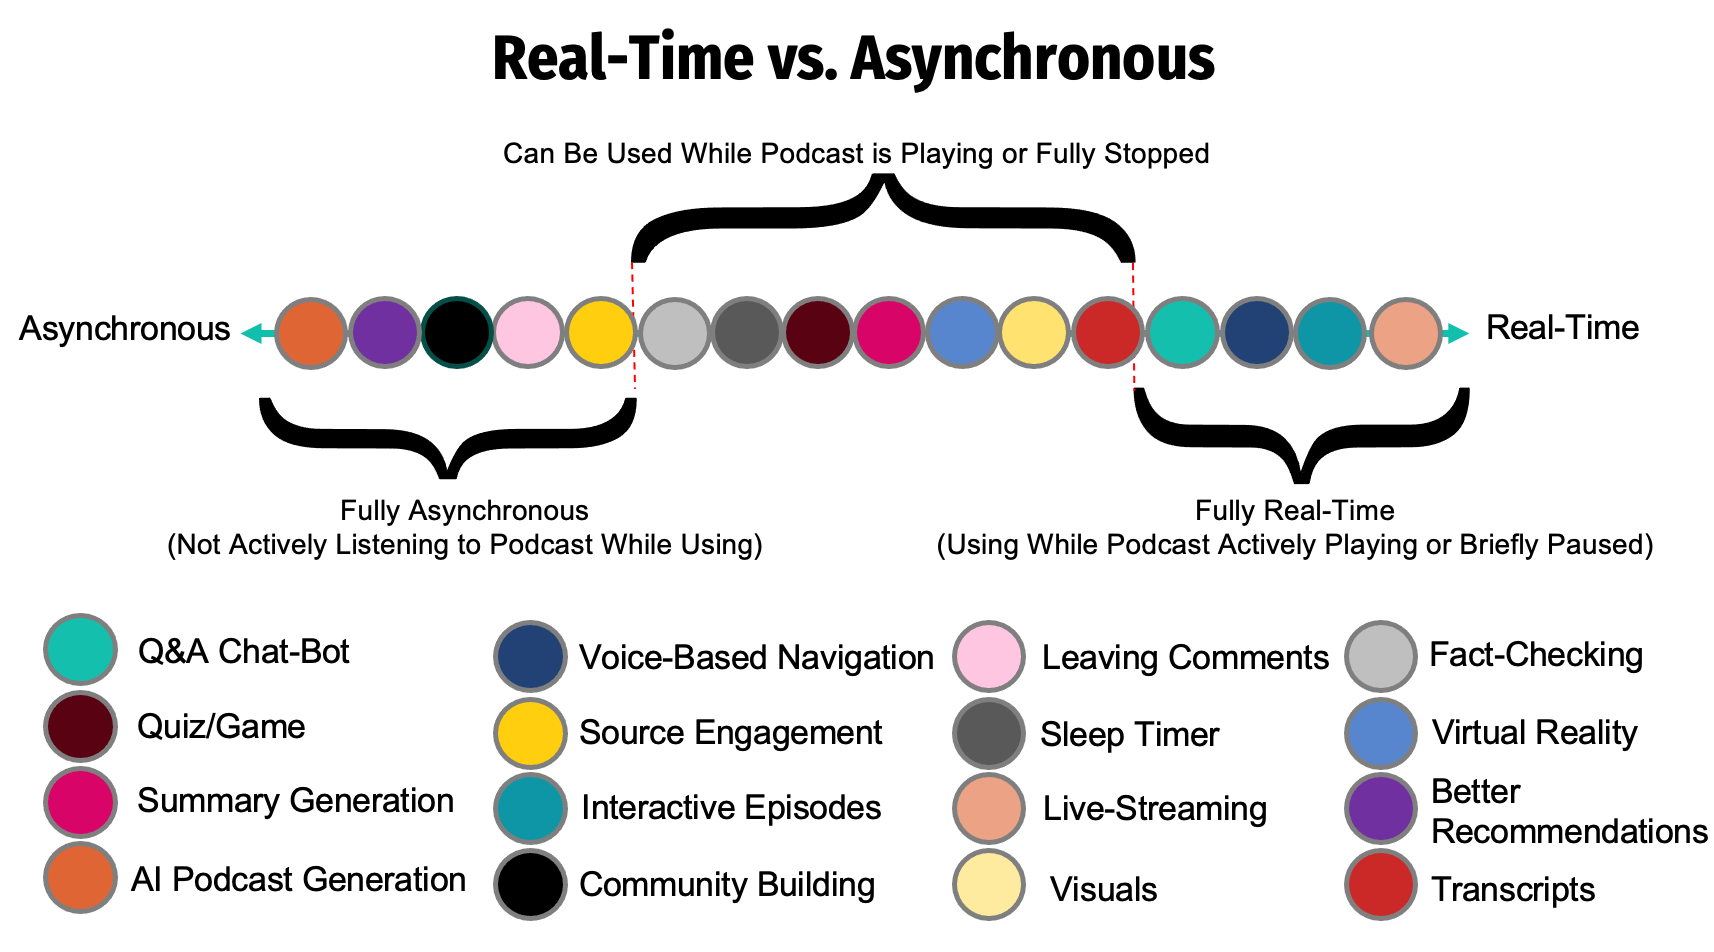
\includegraphics[width=0.9\textwidth]{figures/realtimevsasync.png}
          \caption{The Real-Time vs Asynchronous axis of the listener design space. Features on the right require more instantaneous interaction while listening to the podcast, while features on the left can be interacted with at any point: while taking a break from the podcast or even before or after listening to it.}
          \label{fig:realtimevsasync}
        \end{figure}
        
        The next axis (High Attention vs Low Attention) delineates whether or not a feature requires more or less attention. This axis differs from the previous axis as it is primarily about the cognitive engagement demanded by the podcast's content rather than just the timing of interaction (Real-Time vs Asynchronous). The locus here is both the medium and the message, as this axis revolves around the complexity and engagement level of not only the podcast content but also the specific content, if any, being presented by the interactive feature and the particular manner in which the user must engage with the feature \citep{Sundar2010Designing}. For example, content presented as text directly on a screen may require more attention than content read aloud to the user, indicating implications of the medium. Content or messages that demand higher cognitive resources typically involve deeper, more informative topics that require active listening and processing, such as the full podcast transcript to follow along with versus a summary \citep{GarciaMarin2020}. This axis, therefore, addresses how to design features to hold a listener's full attention or provide a more relaxed, less demanding listening experience. This differentiation helps tailor podcast features that enhance usability according to the listener's available mental resources and preferred engagement level, ensuring a more personalized and effective user experience. A depiction of this axis, along with some representative features, is shown below in Figure \ref{fig:highattvslowatt}.

        \begin{figure}[H]
            \centering
              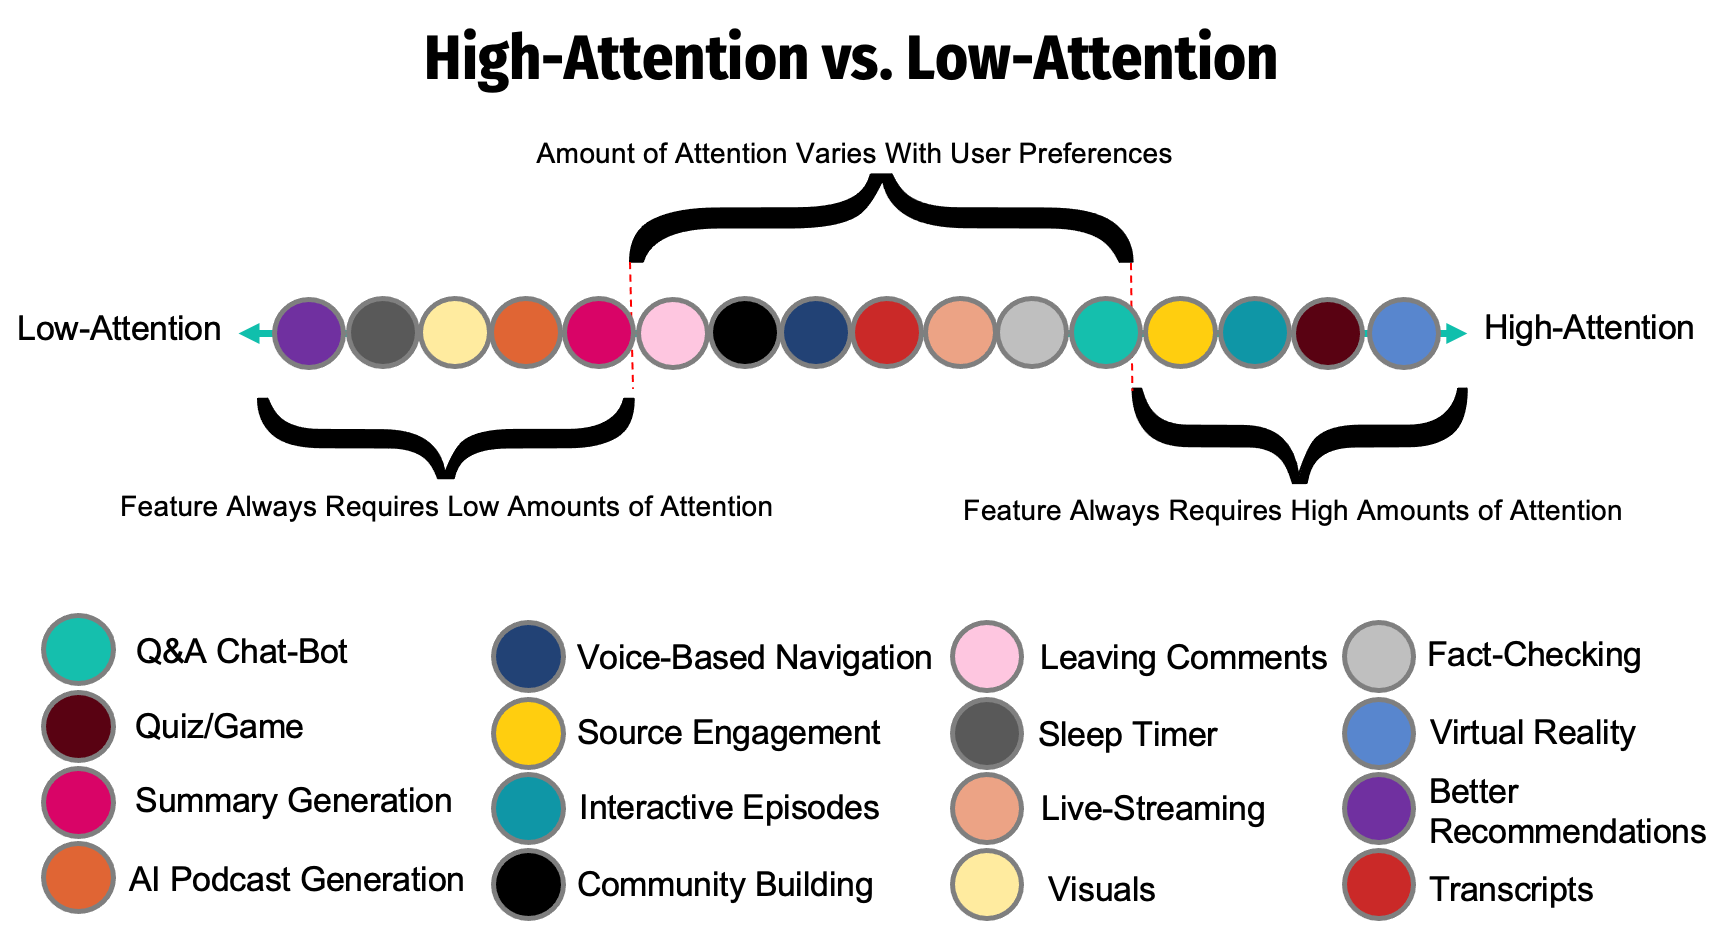
\includegraphics[width=1\textwidth]{figures/highattvslowatt.png}
              \caption{The High-Attention vs Low-Attention axis of the listener design space. Features on the left demand little user attention, while features on the right require the user to focus on the feature while using it. Features in the middle may require varying attention depending on how the user interacts with the feature.}
              \label{fig:highattvslowatt}
        \end{figure}
        
        Lastly, the third axis (Inform vs Entertain) intends to capture the feature's purpose concerning the user's purpose in listening to the podcast. For example, if the listener wishes to learn, features that inform may be more helpful. This axis revolves around the locus of the message, highlighting the distinction between delivering educational, insightful information and providing entertainment or leisure content \citep{Sundar2010Designing}. Podcast features aligned with the "Inform" aspect may include detailed content summaries, access to podcast sources and supplemental resources, or engagement with the podcast transcript. Conversely, features that cater to the "Entertain" aspect might focus on story-telling, user-to-user engagement, or making the podcast experience more gamified. Figure \ref{fig:informvsentertain} further explores this axis, showing how the features identified in the interviews fit along it. Thus, this axis underscores the importance of aligning podcast features with the listeners' motivations, whether seeking to gain knowledge or to be entertained. 

        \begin{figure}[H]
            \centering
              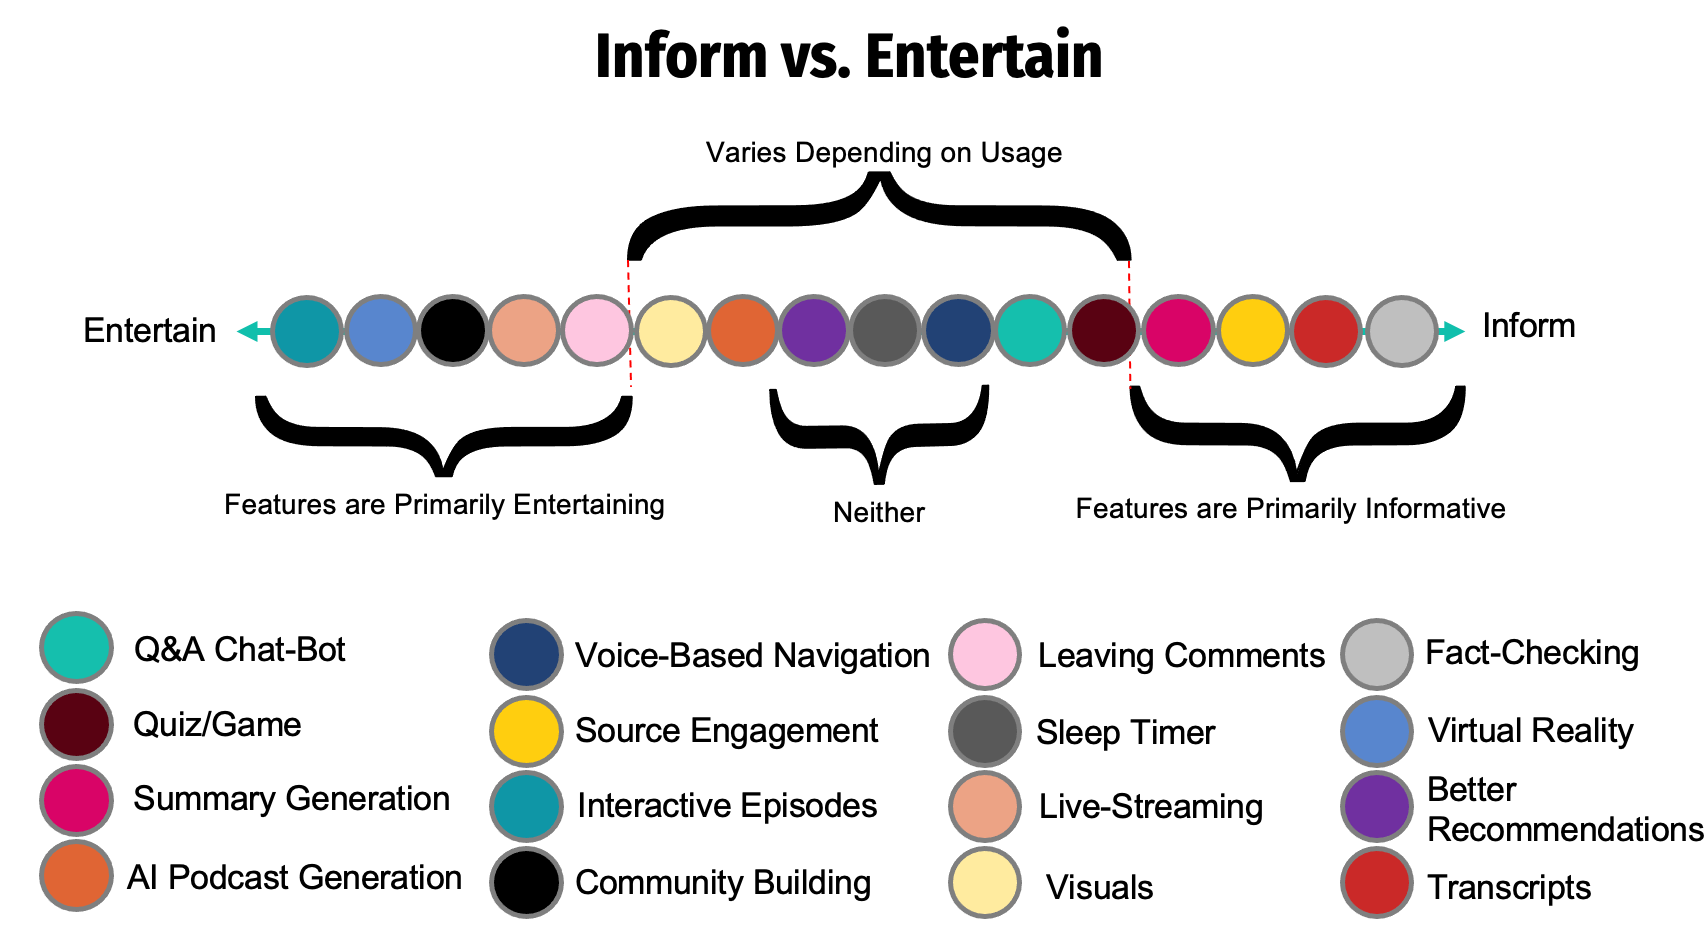
\includegraphics[width=0.9\textwidth]{figures/informvsentertain.png}
              \caption{The Inform vs Entertain axis of the listener design space. Features on the left entertainingly engage the listener, while features on the right provide the user with informative content. The informative or entertaining value of features in the middle depends on how the user interacts with them.}
              \label{fig:informvsentertain}
        \end{figure}

        \indent Figure \ref{fig:listenerds} in Appendix \ref{app:D} shows a limited pictorial representation of the listener design space with a subset of the feature ideas from the formative interviews. This depiction is less ideal than the axis-by-axis breakdown above as the geometry of the cube shape quite constrains it and is full of white spaces that are not populated by the feature ideas from formative interviews. As can be seen, some of the features of the space in Figure \ref{fig:listenerds} do not correspond that well to their placement on the axes; this is because it's impossible to show the inside of the cube, and so features had to be placed on the faces of the cube. Thus, the space in the appendix is more of a visual aid of how the axes can be combined rather than an accurate representation of the design space.
        
        \subsection{Creator Design Space}
        \indent The creator design space also has three axes: Pre-Production vs Post-Production, Creator-Controlled vs Automatic, and Creator-Centric vs Listener-Centric. The first axis defines when the feature is used, similar to the first axis of the listener design space (Real-Time vs Asynchronous). Features can be utilized before production, after the podcast is published, or at either of these stages, depending on usage. This timing affects the workflow and potentially the content's quality and presentation. Figure \ref{fig:preprodvspostprod} shows the interview feature ideas, listed in \ref{tab:creator_design_ideas}, along this axis. Note that the grey circles represent other unidentified features, giving a sense that the design space is continuous. 
        
        This axis is not informed by the same loci as its listener equivalent \citep{Sundar2010Designing}. The type of content that the feature presents to the creator affects when it can be used. For example, retrieving analytics on the podcast's performance before its release makes little sense. However, the medium used to allow the interaction is not informative of when the feature can be used. For example, the Drafting Assistance feature idea is likely in a similar chat-bot format to the Q\&A Chat-Bot, yet their purpose is what informs when to use them.

        \begin{figure}[H]
            \centering
              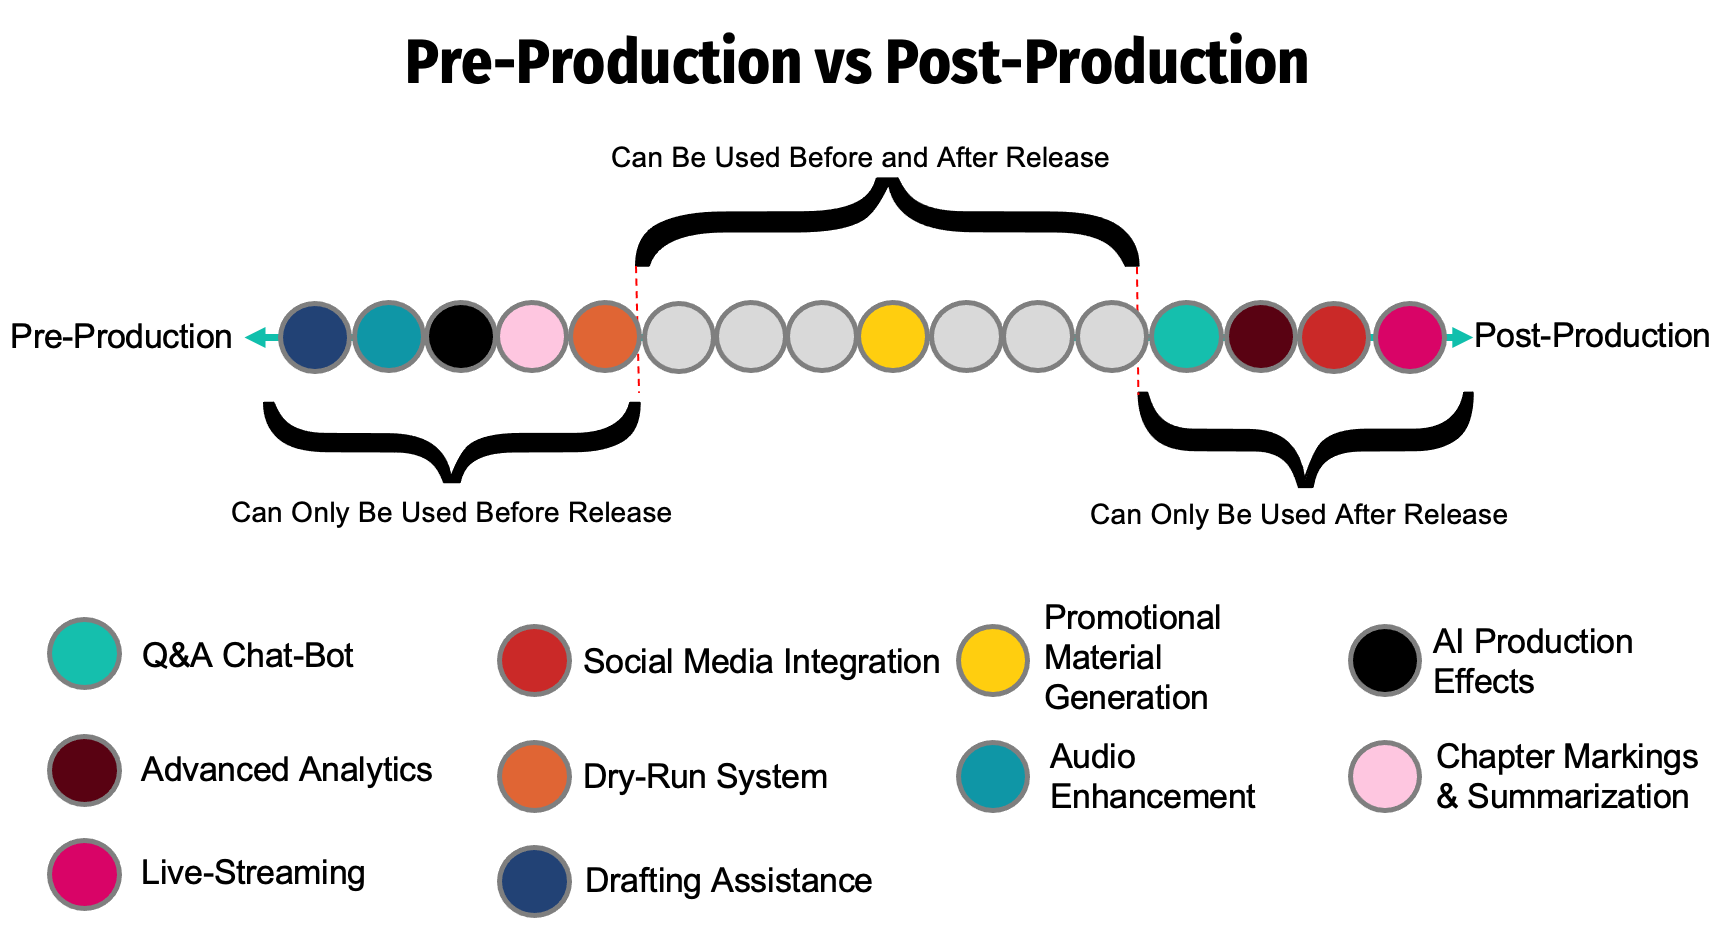
\includegraphics[width=0.9\textwidth]{figures/preprodvspostprod.png}
              \caption{The Pre-Production vs Post-Production axis of the creator design space. Features on the left should be utilized before the podcast is published, while features on the right can only be used after publication. Depending on usage, features in the middle can be used in either scenario.}
              \label{fig:preprodvspostprod}
        \end{figure}
        
        The second axis evaluates how much of the feature relies on creator input or feedback and how much is purely automatic. Creator-controlled aspects require active input and decision-making by the podcast creators, similar to adjusting recording settings manually or editing content personally. This axis mirrors the listener axis on attention because it also deals with active versus passive user input. Thus, this axis is impacted by the same interaction loci of message and medium \citep{Sundar2010Designing}. How the creator must use the feature (the medium in which it's delivered) and what the feature presents to the creator (the message) affect if the creator needs to actively engage with the feature. For example, retrieving analytics is a more automated process that does not require creator intervention and the content it shows the creator does not need to be tweaked or influenced other than to prompt for more or different details. Figure \ref{fig:creatorcontvsauto} depicts this axis.
        
        \begin{figure}[H]
            \centering
              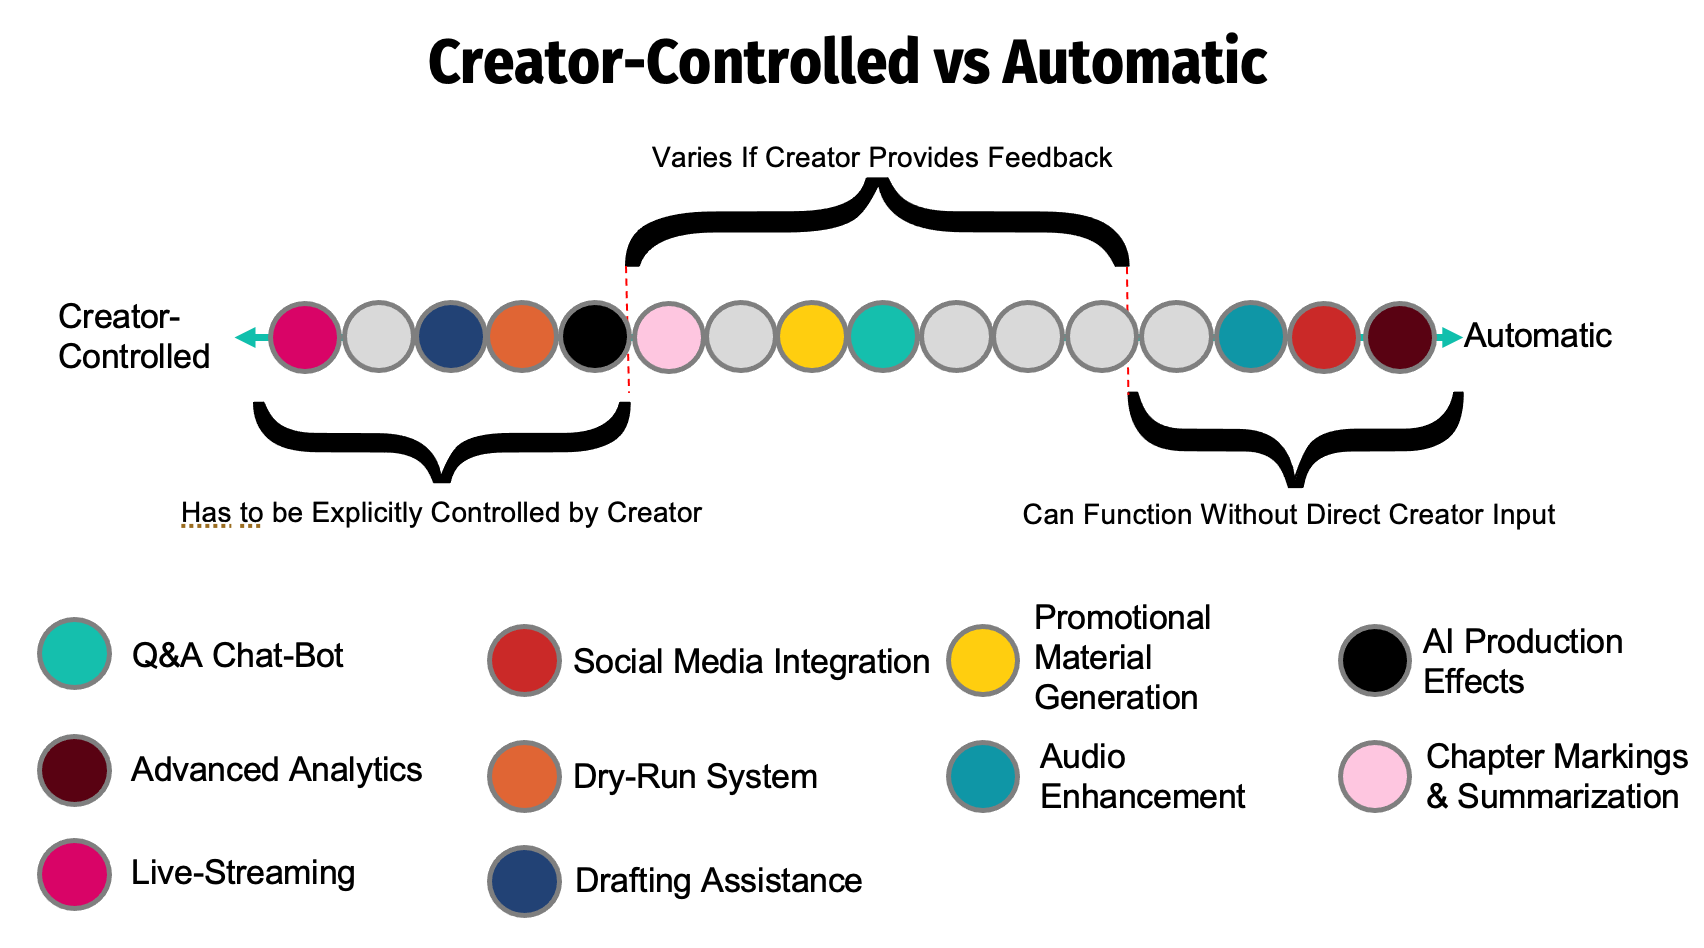
\includegraphics[width=0.9\textwidth]{figures/creatorcontvsauto.png}
              \caption{The Creator-Controlled vs Automatic axis of the creator design space. Features on the left require creators to intervene or directly engage with the feature for it to work, while features on the right require little to no creator input. Features in the middle may require varying attention depending on whether the creator provides feedback.}
              \label{fig:creatorcontvsauto}
        \end{figure}
        
        Lastly, the final axis is once again related to purpose; listener-centric features involve audience engagement and interaction, while creator-centric features involve the creator's podcasting process and interactions with the podcast itself. The interaction loci on which this axis is based differ from those used to develop the Inform vs Entertain axis. This axis depends on both the message and the medium of the interaction rather than the message alone. The message or content of the interaction informs the purpose of its usage, i.e., if the content is more valuable to creators than listeners or vice versa. The medium is also essential as it defines how listeners and creators can utilize the feature. For example, listeners will not have access to the Drafting Assistance feature. The medium itself does not allow this to happen. Figure \ref{fig:creatorcentricvslistenercentric} likewise shows how the other features measure up along this axis. The placement of features on this axis directly relates to each feature's value to listeners and creators alike. Notice that features on either side may still provide value to both parties. For example, as stated above, the Drafting Assistance feature would not be usable by listeners. However, the better quality drafting such a feature provides, the content locus of the interaction leads to a better podcast for the listener to engage with. 

        \begin{figure}[H]
            \centering
              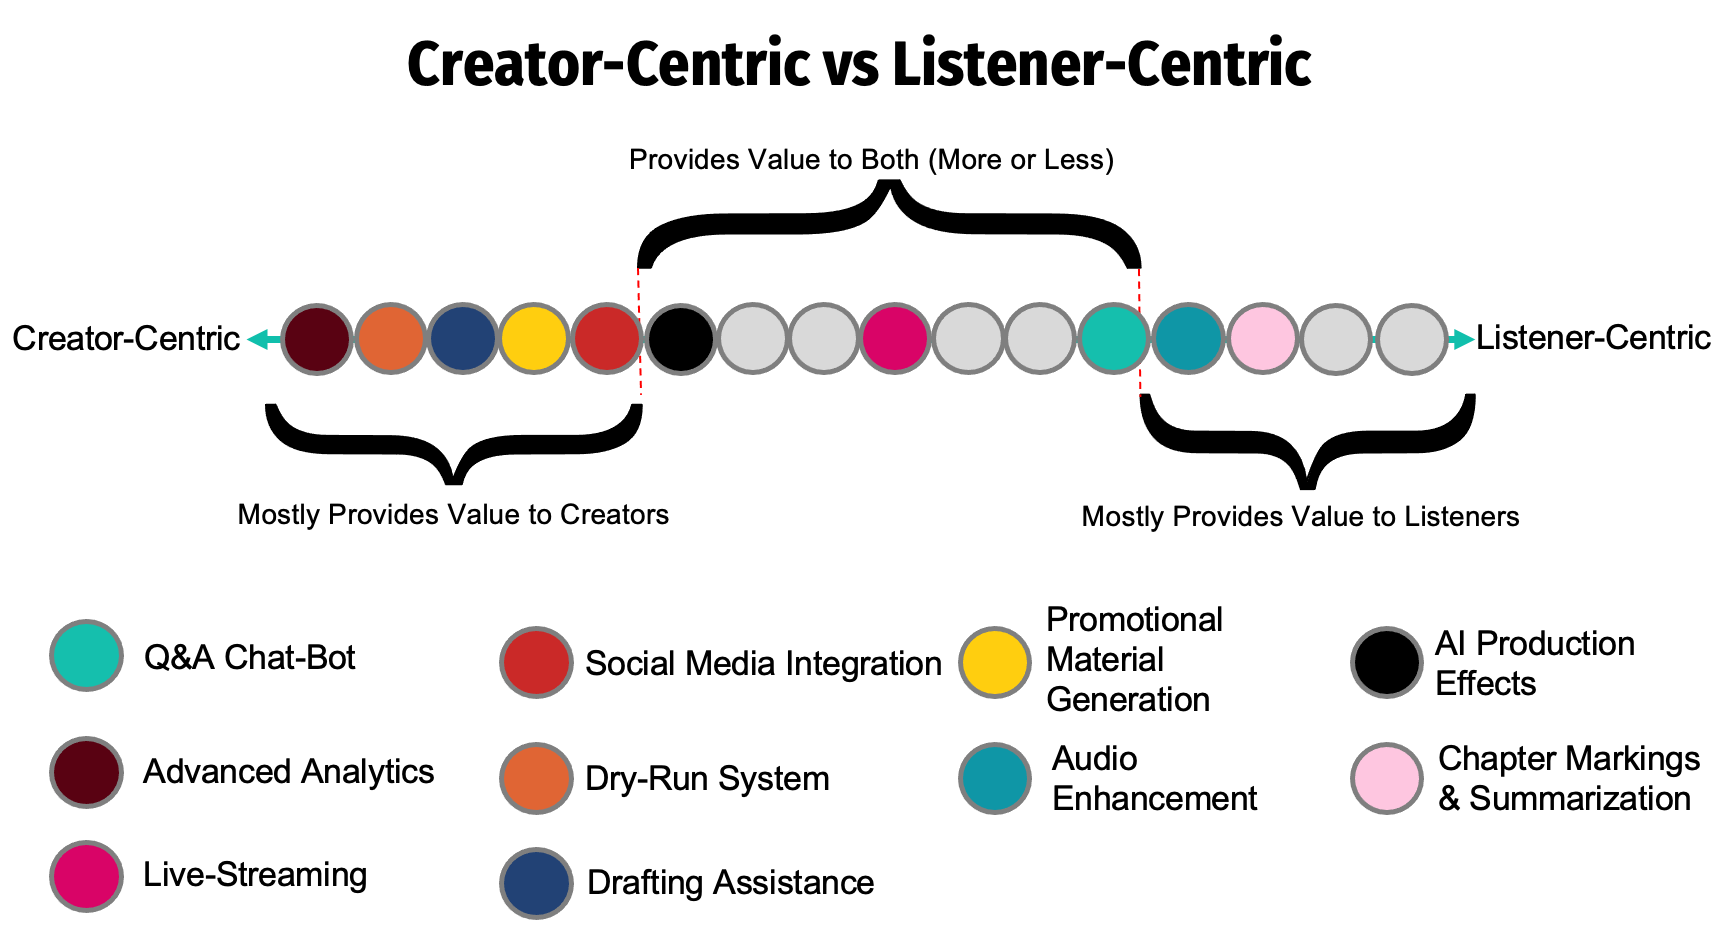
\includegraphics[width=0.9\textwidth]{figures/creatorcentricvslistenercentric.png}
              \caption{The Creator-Centric vs Listener-Centric axis of the listener design space. Features on the left provide more inherent value to creators, while features on the provide more value to listeners. Features in the middle provide a balance of value to both. Features along the axis can still provide value, if minimal, to either user group.}
              \label{fig:creatorcentricvslistenercentric}
        \end{figure}

        \indent Figure \ref{fig:creatords} in Appendix \ref{app:D} shows what these axes would look like when put together. Once again, note that the features on this figure do not fully align with their places on these axes due to the geometry limitations. Therefore, the presented axis representation is the complete representation. 
        
        \section{Real-Time Question and Answering}
        \indent As highlighted above, the axes of the creator design space are analogous to the axes of the listener design space. Thus, a robust design that allows for interactivity between the listener, content, and creator lies in the middle of the creator-centric and listener-centric axis and considers the dynamic preferences of listeners while not overburdening creators.
        
        \indent Thus, a feature idea that fits these criteria and is popular with the interview participants is the Real-Time Question and Answering chat-bot. This feature is poised to tackle two significant shortcomings of the current podcast experience. First, as identified in the formative interviews, users want to better connect with the creators of the podcasts they love to listen to. They want answers to their questions and comments that are often buried or entirely on other platforms. Creators find answering every question a nearly impossible task at worst and an extremely time-consuming and tedious task at best. Creators did specify that such a feature would need to be enabled by the creator on their specific podcast as a whole or for a particular podcast episode, especially if it clones the creator's voice. Both listeners and creators wanted to improve the quality of responses from such a system. In doing so, creators will see what questions are being asked of their content, allowing them to fill in any gaps in future episodes. They will also be able to vet responses for any misinformed or damaging trends. Feedback from listeners would provide an additional influence on response realism and effectiveness. Thus, a feedback loop between listeners and creators is established, which, along with giving listeners simulated access to creators for their questions, fosters a novel, indirect form of interaction. Figure \ref{fig:bridging_the_gap} summarizes this idea while re-iterating statistics from the formative interviews that support the popularity of such a feature amongst listeners and creators alike.

        \begin{figure}[H]
            \centering
              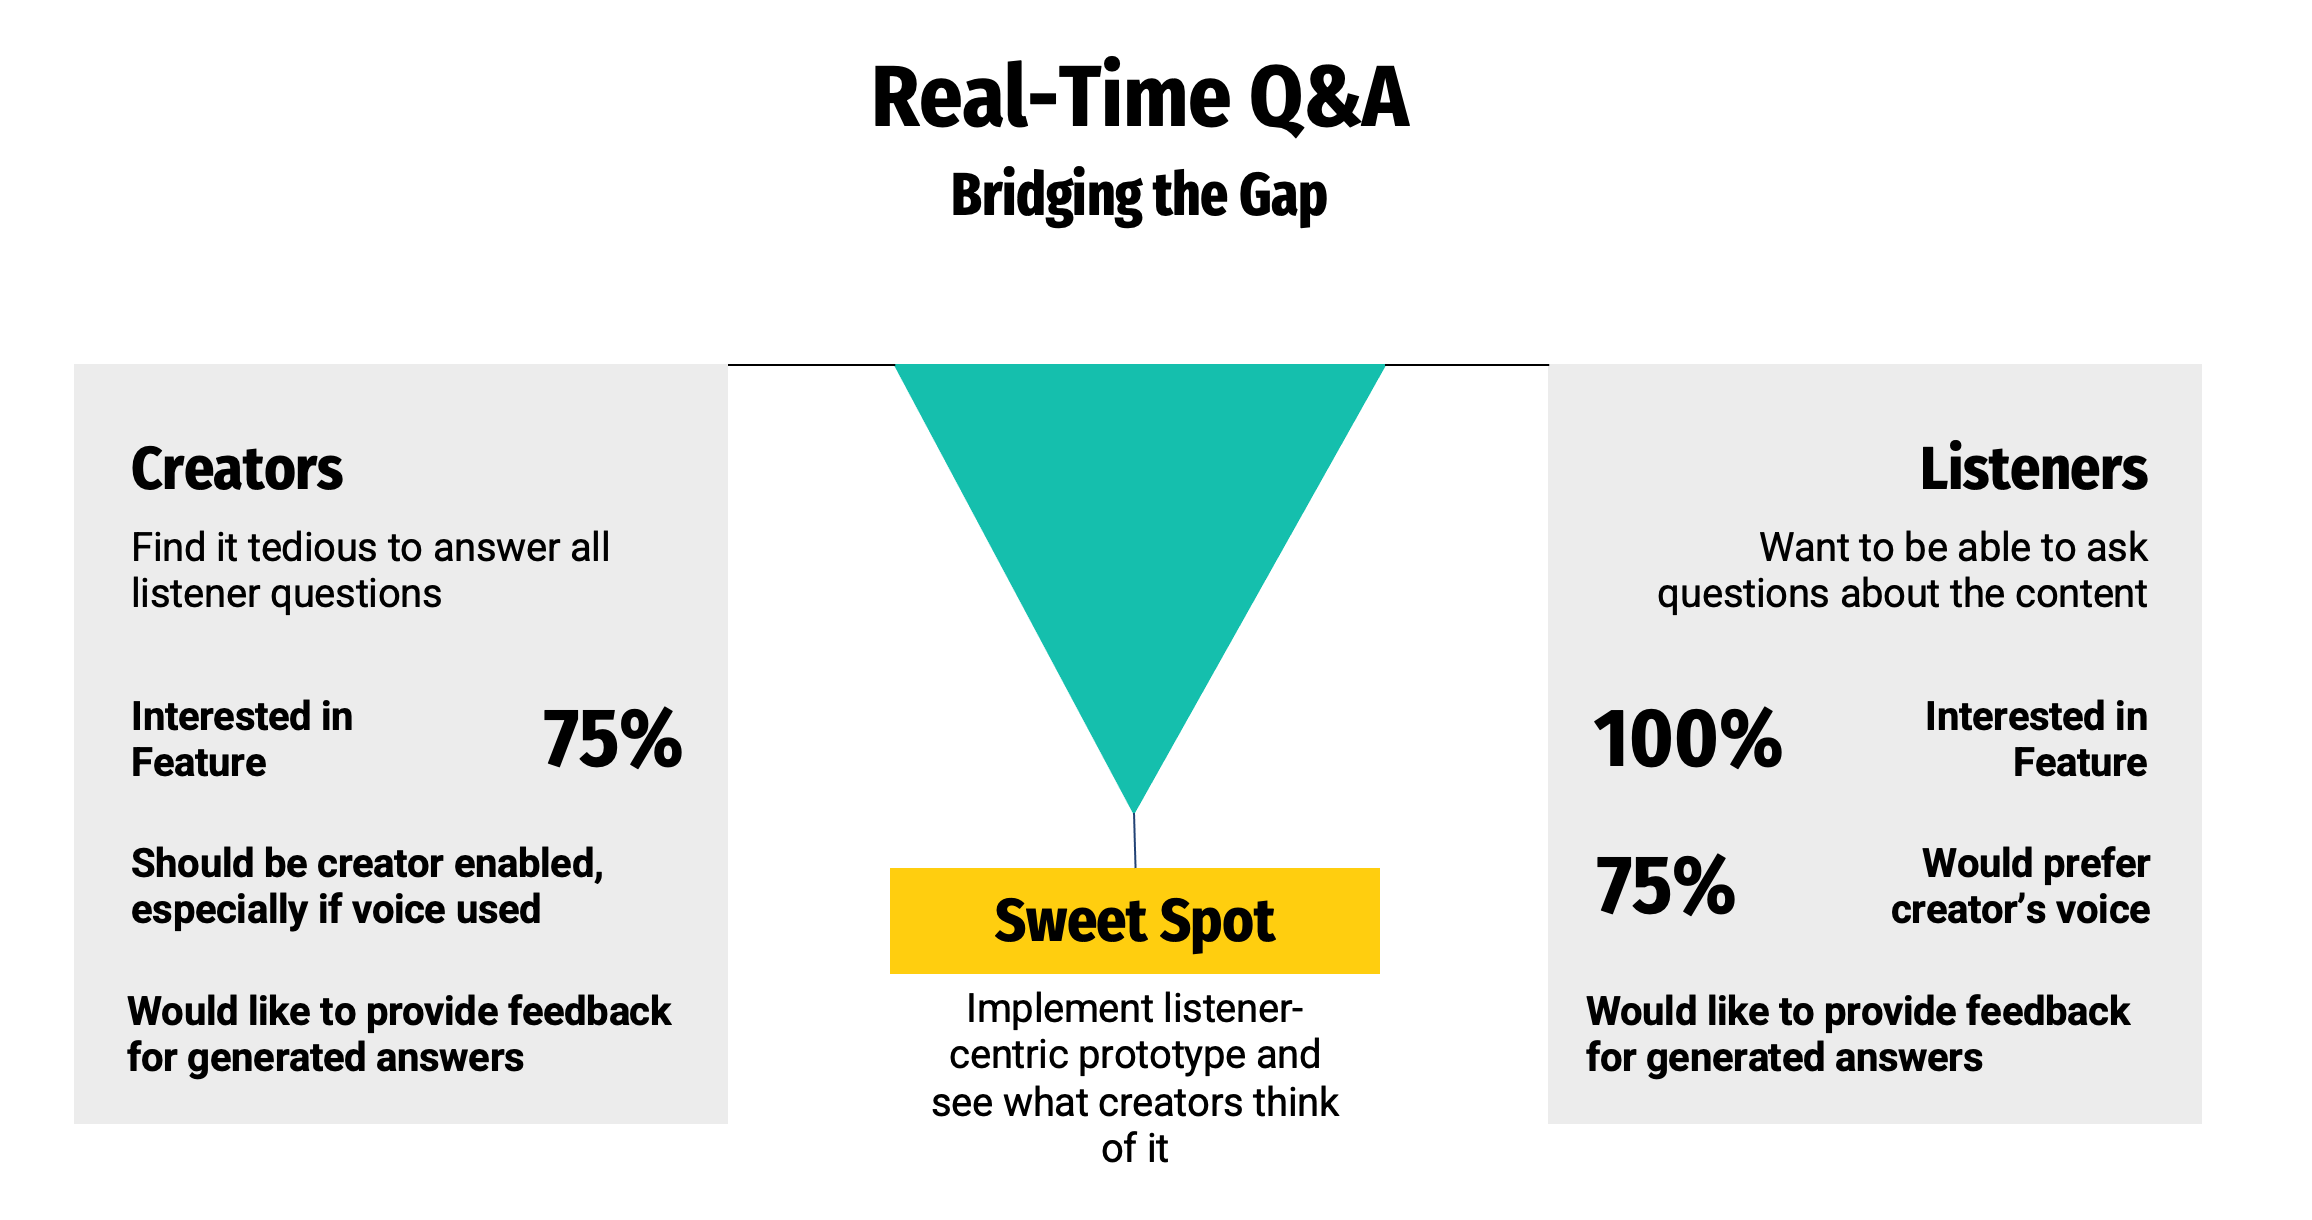
\includegraphics[width=0.9\textwidth]{figures/bridging_the_gap.png}
              \caption{The Real-Time Question-and-Answering Chat-Bot feature has the potential to bridge the gap between podcast creators and consumers. Each side of the diagram shows each group's interest level and the important considerations they raise. The middle of the diagram highlights a clear path forward for design.}
              \label{fig:bridging_the_gap}
        \end{figure}

        As depicted in the figure, we can also establish value for creators by focusing primarily on the listener's experience when developing such a feature. Approaching the design in such a manner benefits listeners directly while, at the minimum, alleviating some of the pain points of creators. Conducting a user study following the development of the system can act as a preliminary feedback mechanism, as described above. If successful, a formal feedback system would be implemented as the design is scaled up to serve on a traditional podcast platform.
        
        \section{Design Goals}
        Following the formative interviews and design space formulation, five design goals were developed to lay the foundation for \textit{ReciproCast}, a real-time question-and-answering system for podcasts. 
        
        \paragraph{D1. Enable Multi-Modal Interaction:} Design the system to support both voice and text interactions for querying podcast content, allowing users to engage in the most convenient mode based on their current activity or environment. This includes allowing the user to use both voice and text and having the system's responses be delivered audibly and via text. This feature also enhances accessibility for those with unique struggles with particular interaction modalities. 

        \paragraph{D2. Provide Authentic and Consistent Responses:} Utilize generative systems that mimic the person prompted to respond closely. Ensure that answers are always 'in character' regarding presentation and content. Implement voice cloning technology to foster a more personal and engaging listener experience.
        
        \paragraph{D3. Develop Real-Time Responsiveness:} Ensure the system can parse listener queries and deliver responses as quickly as possible, enhancing the interactive experience without disrupting the continuity of the podcast content. Allow for features to be interacted with while the podcast is playing and while it's paused.
        
        \paragraph{D4. Optimize for Contextual Understanding:} Incorporate advanced natural language understanding capabilities to ensure the system can interpret the context of listener queries accurately and provide relevant information or responses based on the current podcast content.

        \paragraph{D5. Ensure Ethical Use of Creator Personas:} Implement safeguards against responses that misrepresent the creator and those that contain misinformation or toxicity. Further, ensure that the use of creators’ voices respects their consent and intellectual property, maintaining ethical standards in user interactions. 

        \clearpage

        \chapter{Design Methodology}
        Following these design goals, \textit{ReciproCast} was developed. \textit{ReciproCast} is a full-stack application that enhances podcast interactivity by using GPT-4 Turbo, specifically \texttt{gpt-4-0125-preview}, as the backbone of a real-time question-and-answering system at the episode level. The front-end of \textit{ReciproCast} is a React web application that provides a user interface, allowing listeners to send questions to what we call "conversational avatars." These avatars represent prominent figures within the podcast that the listener might want to interact with. The responses to the questions asked via the front-end are handled in the back-end Flask server as they are computationally expensive. A pipeline diagram is shown in Figure \ref{fig:pipeline}. The following sections will elucidate all of the processes involved in the functionality of \textit{ReciproCast} in greater detail. A demonstration of \textit{ReciproCast} usage is available for download and review \href{https://github.com/kierankasha/thesis/blob/main/supplementals/Thesis%20Demo.mp4}{here}.

        \begin{figure}[H]
             \noindent
             \makebox[\textwidth][c]{
              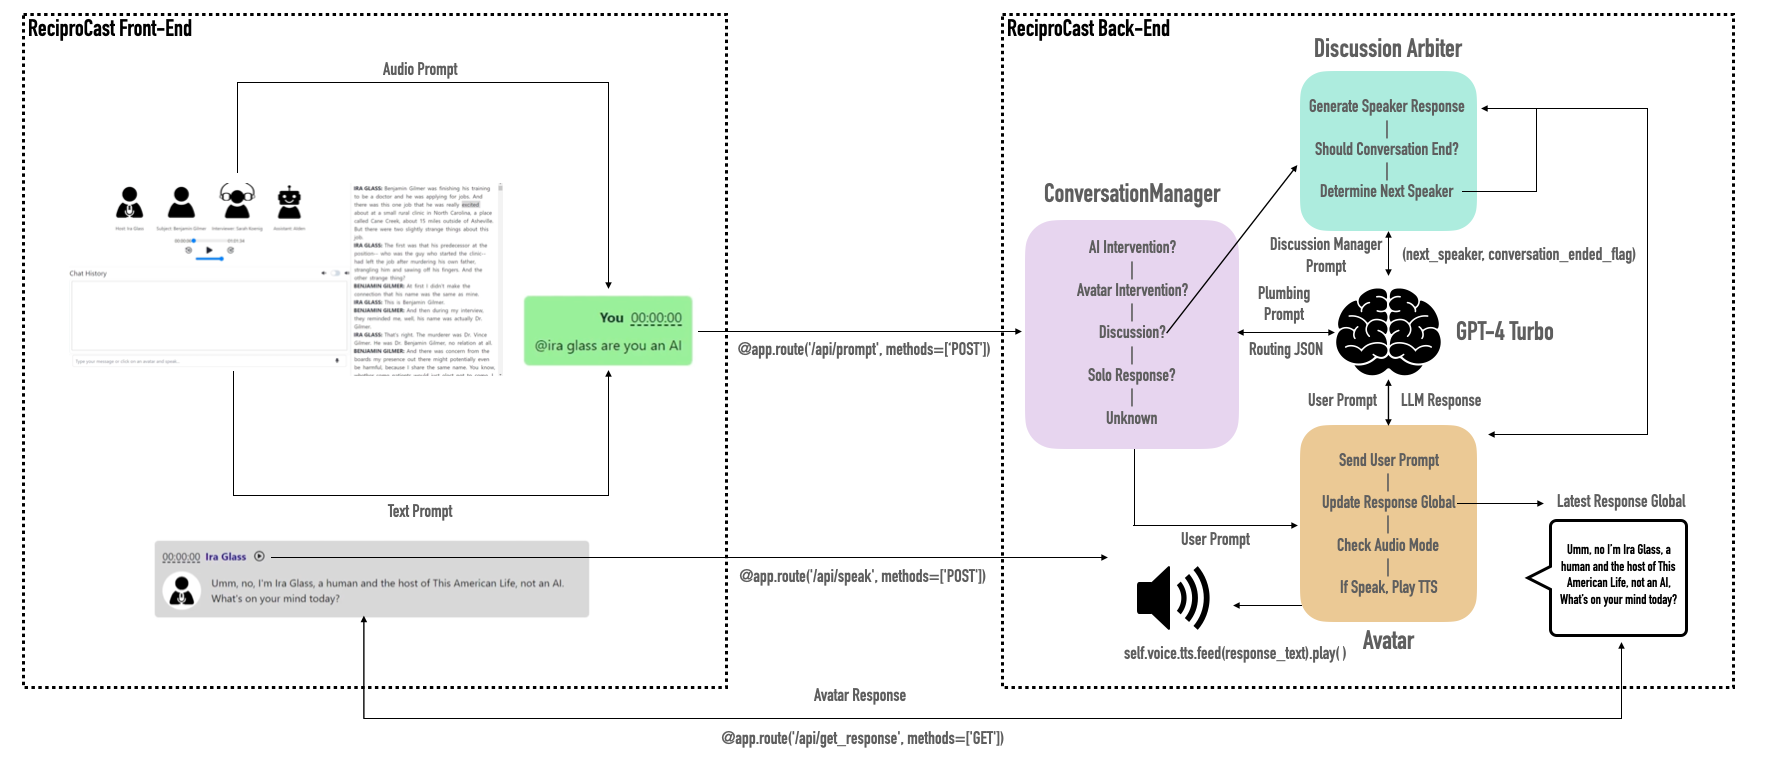
\includegraphics[width=1.3\textwidth, height=0.5\textwidth]{figures/pipeline.png}}
              \caption{The \textit{ReciproCast} system comprises a front-end that handles various user interactions and a back-end that leverages conversational avatars and other LLM calls to facilitate conversation dynamically. This is a high-level overview of the pipeline.}
              \label{fig:pipeline}
        \end{figure}
        
        \section{The \textit{ReciproCast} User Interface}
        The \textit{ReciproCast} user interface is constructed as a React web app via Node.js and CSS. The interface consists of four interactive panels: a media player, a transcript panel, a panel displaying the conversational avatars, and a chat history panel. A view of the user interface with examples of conversational avatars derived from the "Dr. Gilmer and Mr. Hyde" episode of This American Life is shown in Figure \ref{fig:frontend} \citep{ThisAmericanLife2013}.

        \begin{figure}[H]
            \noindent
             \makebox[\textwidth][c]{
              \fbox{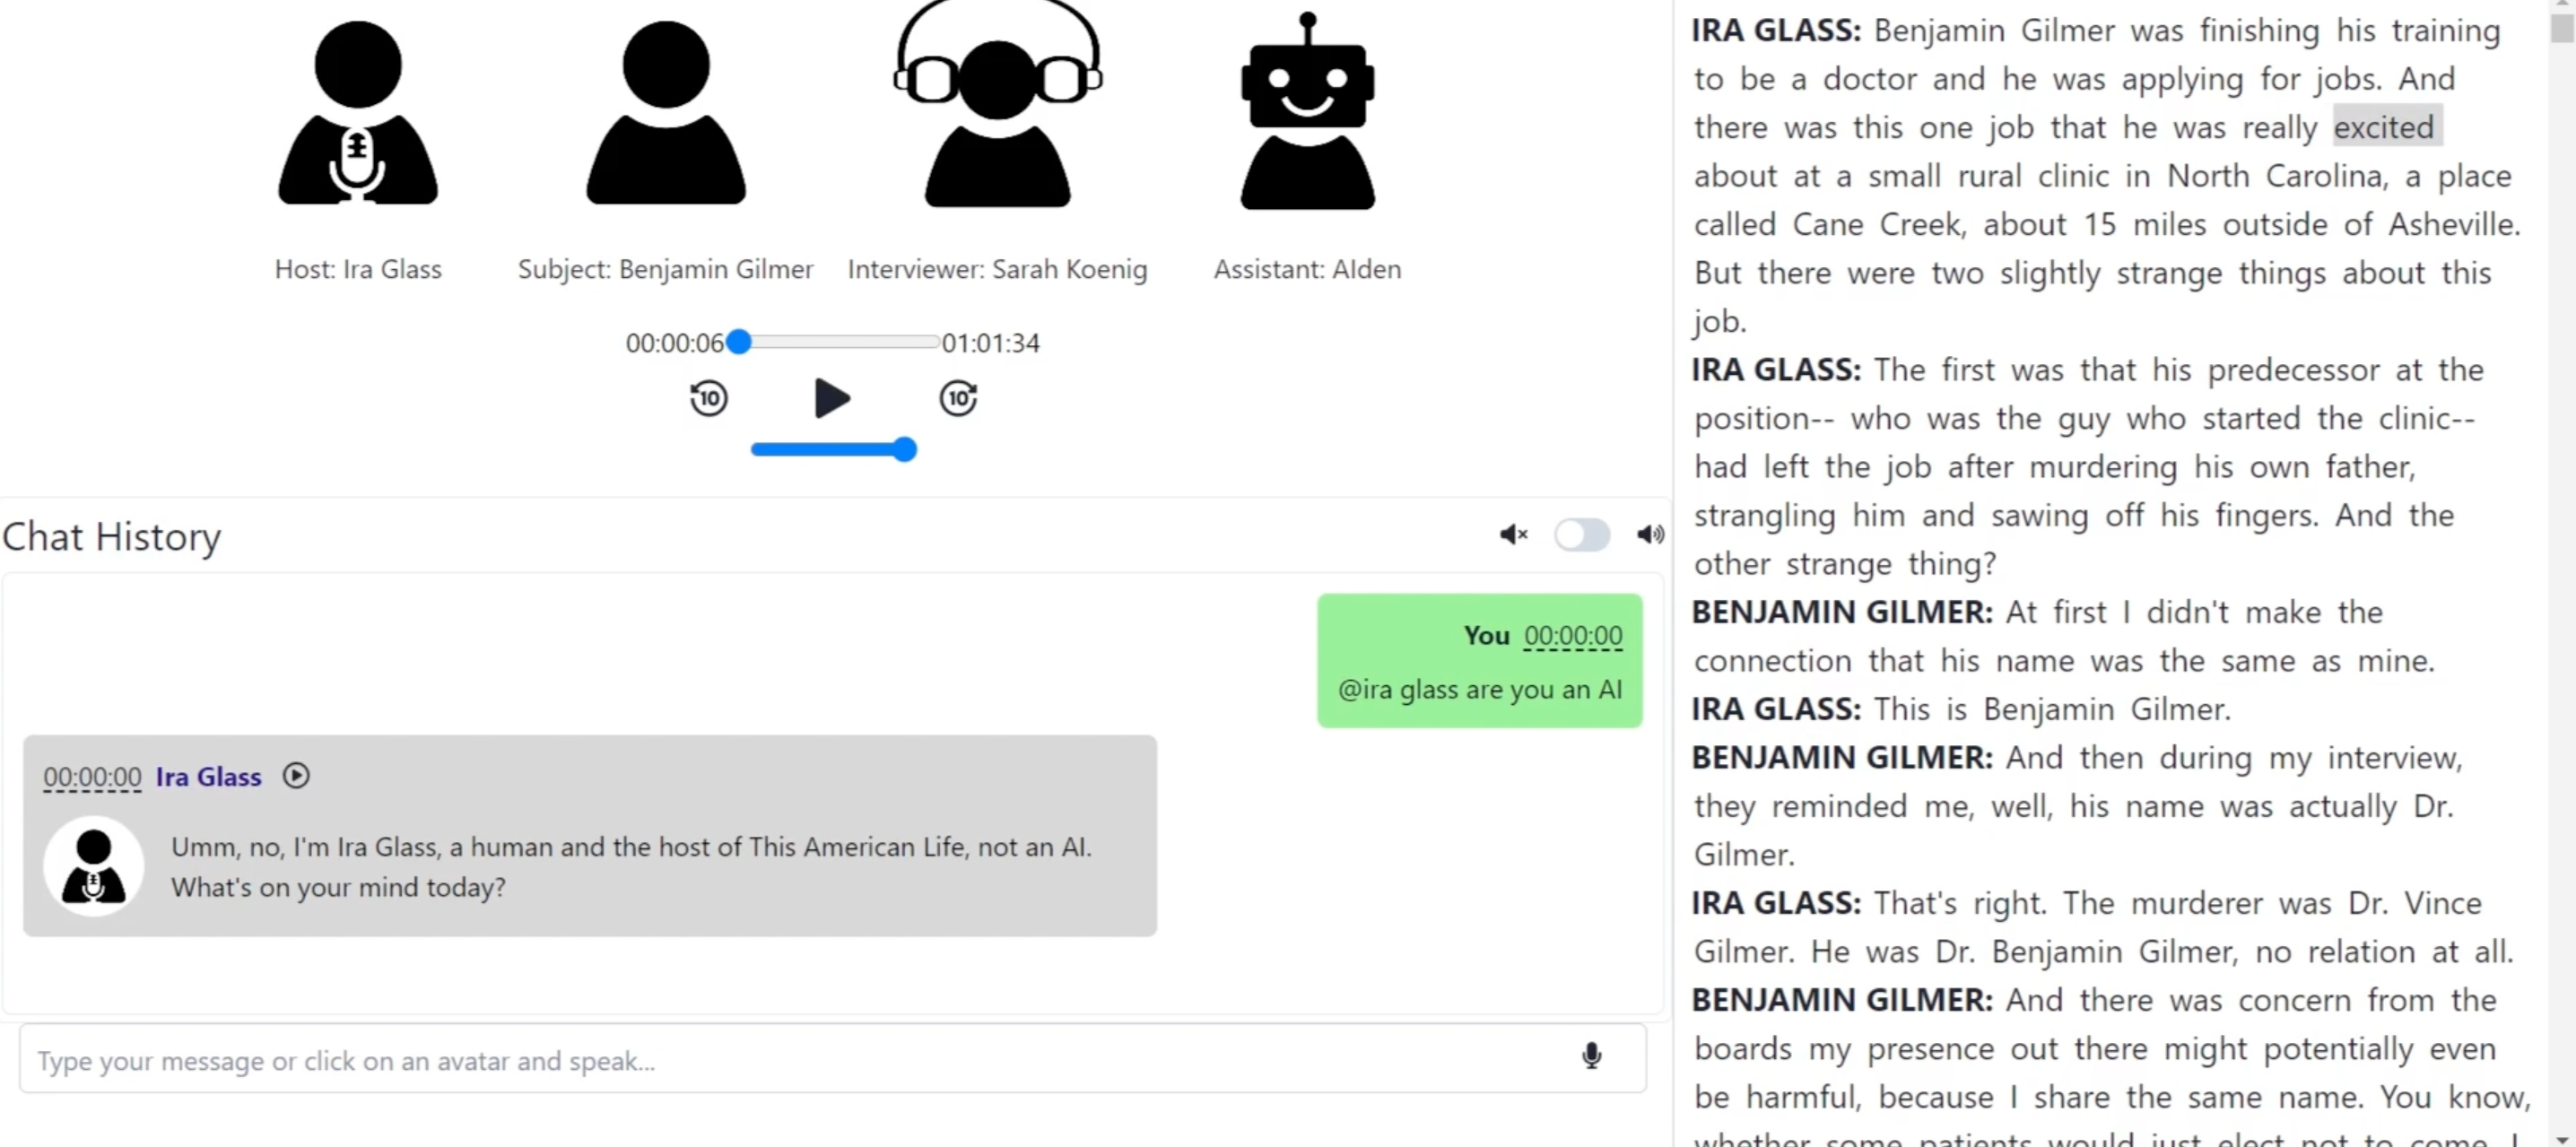
\includegraphics[width=1.15\textwidth, height=0.53\textwidth]{figures/frontend.png}}}
              \caption{The \textit{ReciproCast} user interface, showing the different panels and a sample question and answer pairing.}
              \label{fig:frontend}
        \end{figure}

        \subsection{The Media Player}
        \indent The media player is in a format standard to mainstream podcast platforms. It includes a play/pause button that controls the playback of the podcast episode and a scrub bar that allows the user to click or drag to where they want to go within the episode. The current time within the podcast episode is indicated by the location of the blue dot along the scrub bar. It is also indicated in the timestamp on the left-hand side, with the total length of the podcast located on the right-hand side of the scrub bar. Playback can also be controlled using the icons located to the left and right of the play/pause menu, which skip backwards or forwards for ten seconds, respectively. Lastly, the user can control the volume with the slider below the playback control. The design of this feature relates to \textbf{D3} as it allows the user to control the podcast's playback when interacting with other features. 
        
        \subsection{The Transcript Pane}
        Upon starting the back-end server, the transcript is loaded alongside the audio of the podcast episode. The transcript is presented on the right side of the screen and is in a diarized format such that the words are split up in terms of the speaker, like a script. The transcript is stored in the back-end in a JSON structure inspired by a dataset collected by Huanru Mao \textit{et al.} \citep{Mao2020SpeechRecognition}. Appendix \ref{app:E} presents an example of this JSON structure. For the project, podcast transcripts were generated if they did not already exist and then were formatted in this manner. The benefit of this approach is that the transcript can be leveraged to implement several features. The first is that since each word is aligned to specific time stamps within an utterance, we can highlight the words on the transcript as they are spoken, allowing the user to follow along visually and aurally. This effect is seen in Figure \ref{fig:frontend}. When the highlight reaches the bottom of the transcript pane, the pane automatically scrolls down to adjust. Another significant feature implemented using the transcript is the ability to click on specific words and have the podcast audio jump to when that word is said. This feature allows for much faster navigation than guessing and checking with the scrub bar. The only limitation of these features is the accuracy of the word alignments. However, having the transcript in a JSON format allows these values to be easily adjusted with simple scripts. Thus, this panel and the media player are what a typical podcast platform provides.
        
        \subsection{The Avatar Panel}
        \indent The Avatar Panel, shown more in detail in Figure \ref{fig:avatarpanel}, sits at the top of the user interface. The avatars populate in the front-end as they are set up in the back-end on server start-up. Users can click on the avatar icons, which puts them in a spotlight to indicate who is being interacted with. Doing so activates the user's microphone for speech recognition, directing what they say to that specific avatar by adding a tag with the avatar's name to the start of the user's prompt (e.g. @Ira Glass). Clicking on a different avatar while another is highlighted deletes the previous message, restarting the speech-to-text system for the new avatar. 
        
        \begin{figure}[H]
            \makebox[\textwidth][c]{
            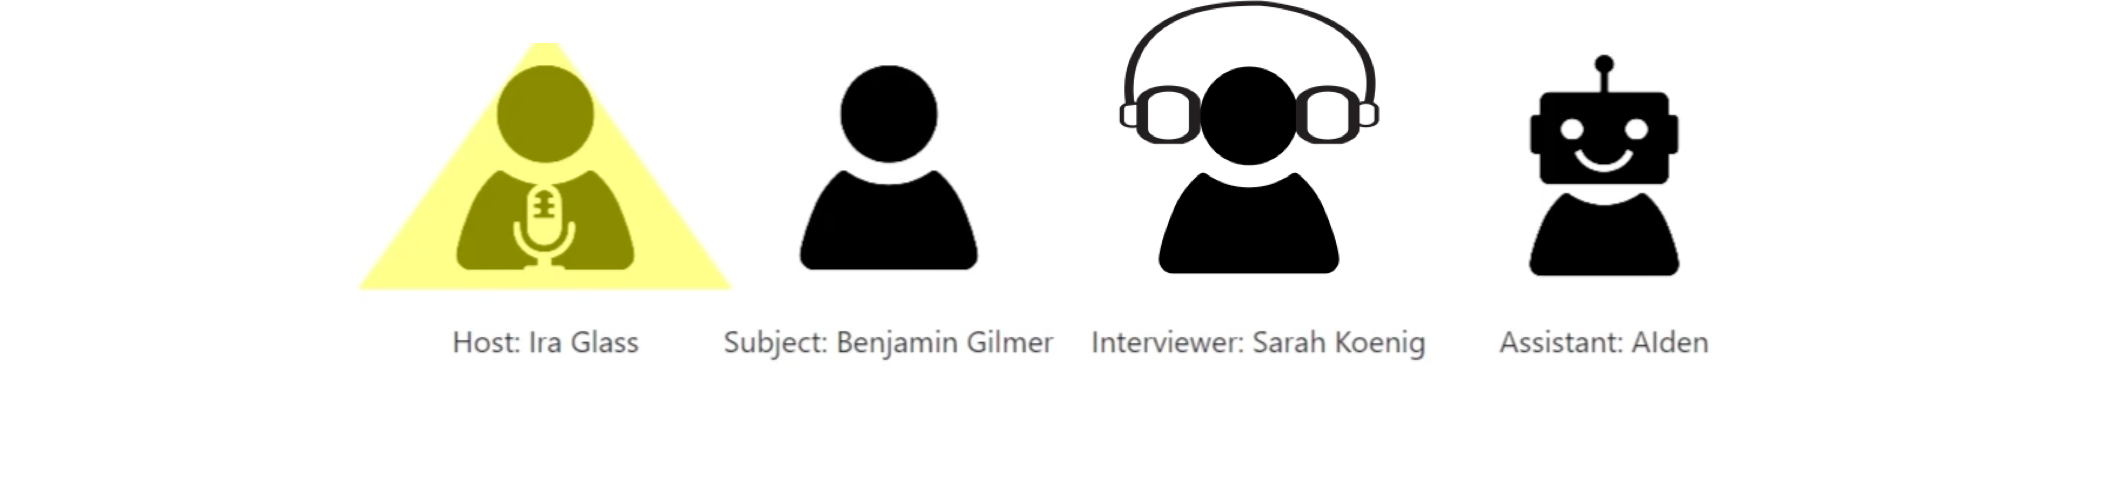
\includegraphics[width=1.5\textwidth]{figures/avatarpanel.png}}
              \caption{Clicking on an avatar highlights the one clicked on and activates the microphone.}
              \label{fig:avatarpanel}
        \end{figure}
        
        \indent As can be seen, each avatar represents a person within the podcast and has an icon depicting their role. For podcasts with many people, like This American Life, the system is limited to one avatar per role due to computational limitations. However, the system allows for more than one avatar in a role on podcasts with a smaller scope, especially in more traditional 'panel-style' podcasts. The Host role represents the narrator or podcast lead. They typically expound more expository speech or ask questions in the studio setting \citep{Mao2020SpeechRecognition}. Some podcasts are comprised of several co-hosts facilitating discussion. The Subject role is the person being interviewed or the main focus of the podcast episode \citep{Mao2020SpeechRecognition}. The Interviewer role represents an 'in-the-field' reporter who conducts interviews directly on the ground rather than in the studio space \citep{Mao2020SpeechRecognition}. This role is commonly found in many podcasts produced by media corporations or news stations as a proxy for legacy programmes. AIden is a generic AI assistant meant to answer questions the user may not need or want to direct toward the human-based avatars.
        
        \subsection{The Chat History}
        \indent The Chat History pane has two major components: the text box and the chat room. The text box allows users to type their prompts rather than to speak them. The text box automatically stretches vertically to accommodate longer prompts, allowing users to scroll through them. If the user is unhappy with the prediction the speech recognition system makes of what they said, they can directly edit the prompt in the text box as these predictions show up in the text box as they speak. Doing so stops speech recognition altogether. Users must press the Enter key to submit all prompts, whether from speech or written manually. They can, however, Shift-Enter to add a new line to their prompt. Users cannot submit a prompt while waiting for a response to arrive; this prevents collision cases where responses may show up in unexpected orders in the chat room and may cause issues with the text-to-speech. Lastly, the text box contains a microphone icon. This icon turns red when speech recognition is active, and it happens when users click an avatar icon or when they click the microphone button itself. In the latter case, this activates speech recognition without directing the prompt at any particular avatar. In both cases, when the user is finished using the speech recognition, they can hit Enter or click the microphone button again. Thus, the text box and the avatar panel allow multi-modal interaction with the \textit{ReciproCast} system, inspired by the first design goal \textbf(D1).  
        
        \indent The chat room component of the pane shows all messages sent between the user and the avatars since the last page refresh. The window is scrollable, allowing users to refer to previous messages easily. After sending a prompt, the user's message appears in the chat room in green and on the right-hand side of the screen to help differentiate it from the avatar responses. The message and all responses include a timestamp representing the podcast's playback time when the prompt was sent. This timestamp is clickable, allowing users to backtrack to where they were when they asked the question. Figure \ref{fig:chathistory} shows the Chat History feature in more detail. 

        \begin{figure}[H]
             \fbox{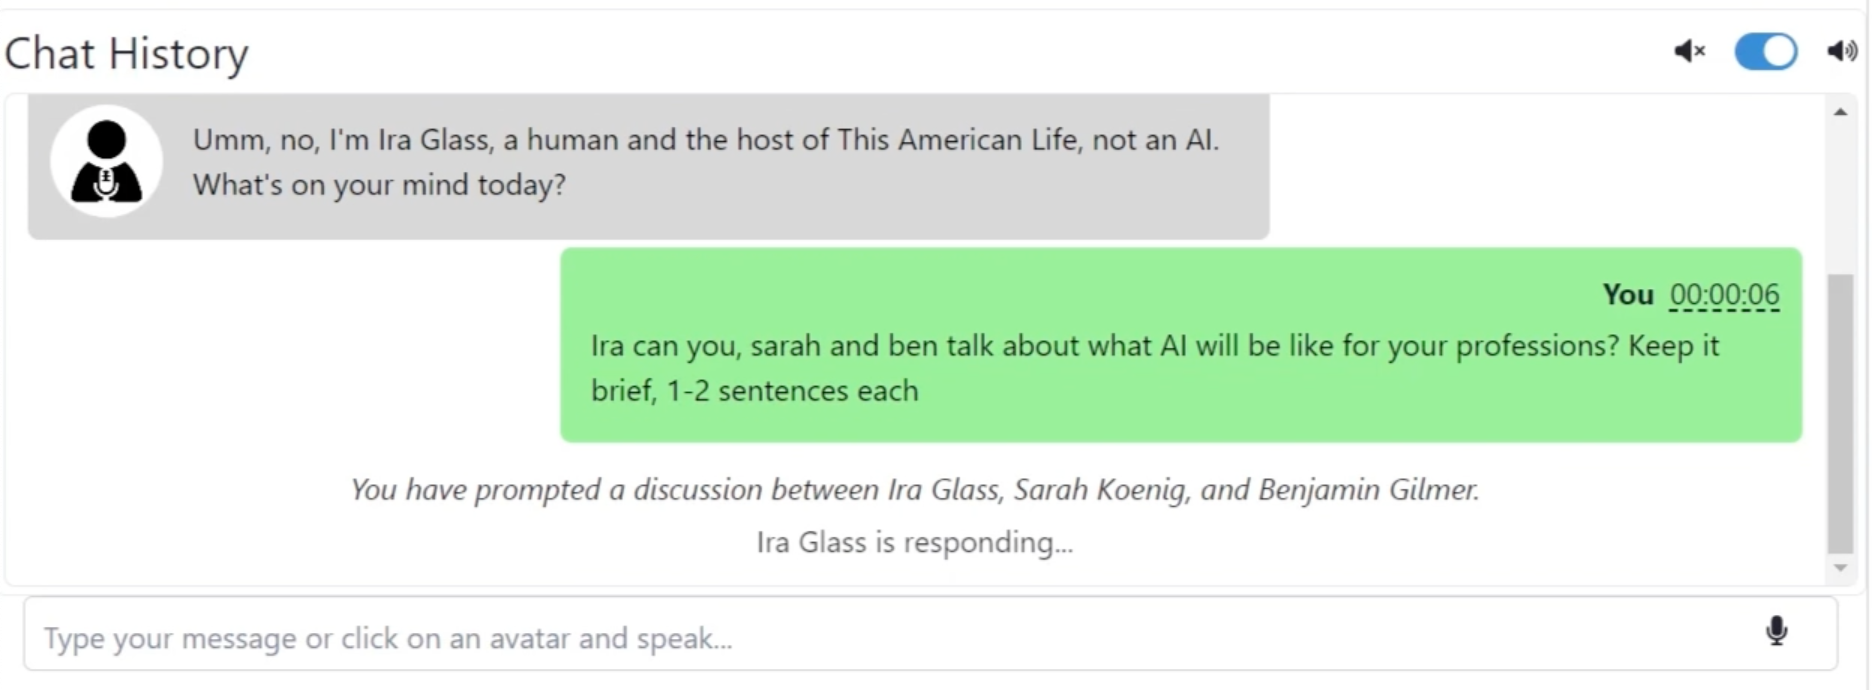
\includegraphics[width=1\textwidth]{figures/chathistory.png}}
              \caption{The Chat History feature with a sample prompt.}
              \label{fig:chathistory}
        \end{figure}

        \indent The figure shows a critical design choice: once the user's response has been successfully routed in the back-end, a message is displayed that shows what kind of conversation their prompt has initiated and which avatar, or avatars, will respond. Following this, text flashes describing which specific avatar is currently responding. This message disappears once the response from that avatar is received. The purpose of this is to provide transparency to the user regarding what to expect from the responses to their prompt. 
        
        \indent The responses from avatars each have the role icon of the avatar responding and the avatar's name. The colour of the name is chosen via a unique hash, prioritizing darker colours. The distinct colour allows the user to better differentiate different avatars that may have the same role icon. Further, responses may include references to the podcast transcript. These references are sent from the back-end, given the response generated by the avatar, and allow the user to check against what was actually said within the podcast. This feature was based on \textbf{D2} as it authenticates the responses. As seen in Figure \ref{fig:transcriptreferences}, these references are links that can be clicked on, and the podcast playback will skip to that part of the episode. These links are stored in a drop-down box that is hidden by default to prevent clutter. Lastly, while human-based avatar responses are grey, AIden responses are blue to help users differentiate them quickly. 

        \begin{figure}[H]
                
\includegraphics[width=1\textwidth]{figures/transcriptreferences.png}
              \caption{Some responses will have references to the transcript that can be clicked on to skip to that part of the episode.}
              \label{fig:transcriptreferences}
        \end{figure}

        \indent Lastly, there are two ways that the user can activate the text-to-speech. Figure \ref{fig:transcriptreferences} shows that each response has a small play button next to the avatar name. This button can be clicked to activate the voice playback of the conversational avatar. The button can be clicked again to pause this playback. After it's been paused for ten seconds, the playback is reset to free up computational resources. The other option is to use the switch shown in Figure \ref{fig:chathistory} on the top right corner of the box. When the switch is flipped on (i.e. towards the volume on icon), the avatars will automatically 'speak' as soon as their response arrives from the back-end. The conversation will then be blocked until the speech is completed to prevent multiple avatars from speaking simultaneously. Speech mode also automatically pauses the podcast episode so the avatar does not talk over the podcast. If switched off, the user has to use the play button on the message to activate speech, and the responses arrive silently, not disrupting the flow of the podcast. This feature directly results from design goal \textbf{D3}, providing users with the direct agency to control where the feature fits on the High-Attention vs Low-Attention and Real-Time vs Asynchronous axes of the design space. Thus, the user can determine how much interaction with the system interrupts the flow of the listening experience.

        \section{\textit{ReciproCast} Back-End Implementation}
        \indent \textit{ReciproCast}'s back-end consists of modular components and is written entirely in Python. The back-end also stores the podcast content, including the audio file and JSON transcript. The most important component is the implementation of the conversational avatars via the \texttt{Avatar} class. The Flask Server component handles all communications with the front-end, allowing \textit{ReciproCast} to function as a full-stack application. User prompts are handled dynamically via a \texttt{ConversationManager}, automatically routing them to the relevant avatars.
        
        \subsection{Conversational Avatars}
        The \texttt{Avatar} class encapsulates and manages each conversational avatar's unique characteristics and memory. Each avatar is backed by GPT-4 Turbo, allowing each avatar to have its own system prompts that encapsulate its personality and purpose. From now on, all references to LLM calls mean utilizing the GPT-4 Turbo API. These system prompts are role-dependent and give the agent access to its name, a description of its role in the podcast, generic instructions for responding believably, and the full podcast transcript. The transcript was created by extracting the utterances from the JSON file and extracting them into a script-formatted text file. The prompts used for the conversational avatars, separated by role, can be found in Table \ref{table:personality-prompts} in Appendix \ref{app:F}. The design of these prompts was directly inspired by the \textbf{D2} design goal. By providing a diarized transcript, role and response expectations, and the avatar's name, this approach ensured that the LLM would always have access to this information to refer to.
        
        \indent This approach to LLM agents is similar to the "Generative Agents" paper, which utilized GPT-3.5 Turbo to create dynamic, non-playable characters in a video game \citep{Park2023GenerativeAgents}. While this research indicated that such a system can generate believable responses to queries, one of the major concerns of any systems utilizing an LLM is that they come with a limited context window \citep{OpenAI2023GPT4}\citep{Park2023GenerativeAgents}. This limitation means that as the context length of the conversation continues to grow with the number of queries, the model may ignore or lose track of important parts of the conversation context, potentially making the model come up with strange, hallucinated, or inaccurate responses. However, utilizing GPT-4 Turbo rather than GPT-3.5 Turbo proved to be more effective as it has a much larger context window of 128 thousand tokens rather than 3.5's 16 thousand \citep{OpenAI2023GPT4}. Thus, an alternative approach was taken to the one presented in the paper, which gives each avatar access to their entire conversation history, which includes their initial system prompt at the start to continuously remind the avatar of their role, personality, and the content of the podcast. To debug that this worked, a method was added to the \texttt{Avatar} class to check the number of tokens in the conversations. This method is called whenever a new user prompt is added to the conversation history, and the result is checked against the context window limit. This bound was never exceeded during testing. The one downside of this approach is that by having each avatar have access to only their conversation history, it means that avatars are not able to refer to discussions the user had with other avatars unless they, too, were part of that discussion. Thus,  while the approach is efficient, tractable, and conducive to high-quality responses, there are potential avenues for further improvement.

        \indent Alongside maintaining ownership over their own conversation history, conversational avatars also have ownership over their voice via a TTSManager class. The RealtimeTTS library is used for this task \citep{RealtimeTTS}. This library is an open-source wrapper around the most powerful speech synthesis and AI-powered text-to-speech (TTS) tools, including OpenAI's TTS, ElevenLabs, Microsoft Azure TTS, and Coqui AI. The library allows for flexible usage of these voice models, or even the user's system TTS, in real-time applications. The library ensures continuous playback by falling back on other voice engines if something fails, providing a consistent and non-intrusive experience. 
        
        \indent Further, RealtimeTTS is configured to work with LLM outputs, filtering out escape characters that may disrupt specific speech models. Lastly, the library was chosen since it allows for a great deal of configuration, including playback speed, sentence pause duration, and synchronous and asynchronous playback modality, including the ability to pause speech altogether \citep{RealtimeTTS}. The Coqui Engine was chosen as the voice model for human avatars using XTTS V2 as the TTS model \citep{XTTS_Coqui}. This choice is because Coqui AI's open-source models can be run locally. Where other speech synthesizers require API calls or for voices to be synthesized in advance, XTTS can run on machine at runtime, requiring as little as 3 seconds of audio to clone a human voice and allowing for usage in multiple languages. When the podcast is loaded in and the conversational avatars are created, the transcript JSON file is parsed to find utterances based on the avatar's name that are longer than 10 seconds as that was recommended for the best results \citep{XTTS_Coqui}. Once this utterance is found, its starting and ending timings are used to trim the podcast audio into a file fed into the voice engine. Once this step is completed, the avatar becomes accessible on the front-end for interaction. For AIden, the generic AI assistant, the OpenAI TTS, is used since there is no voice to clone \citep{OpenAI_TTS}. This TTS model is quite robust, allowing for natural delivery in multiple languages. Thus, leveraging these models and libraries allows \textit{ReciproCast} to deliver on \textbf{D2}, allowing responses the ability to be read in a synthesized version of the voice of the real person in the podcast, as requested by most participants in the formative interviews. 

        \subsection{Flask Routes}
        \indent The \textit{ReciproCast} Flask application has a server module in the back-end that facilitates access to podcast content and conversational avatars from the React front-end. Figure \ref{fig:flaskroutes} shows a diagram of these routes.

        \paragraph{Podcast Content Routes:} For accessing podcast content, the application includes endpoints that allow the front-end to retrieve the podcast sources dynamically and directly through URL requests.
        
        \paragraph{Avatar Routes} The server module also supports retrieving a dictionary of avatar names and roles as they are loaded. This information allows the front-end to update the Avatar Panel with the icons of the available avatars. The server also facilitates receiving user prompts from the front-end, which are then routed to the appropriate avatars dynamically. The server routes also allow users to control the speech synthesis of avatars. This includes starting speech playback via the play/pause button on the response messages, pausing, and resuming this playback. When the speech mode is activated in the front-end so that the avatars automatically speak, this is handled as soon as the response is received from the LLM in the \texttt{response} method of the \texttt{Avatar} class.
        
        \paragraph{Polling Routes} Lastly, the application supports several polling mechanisms to keep the front-end updated about the current state of conversations. This is achieved by maintaining a global state in the back-end when specific routes are accessed. Two main routes control the flavour text shown in the chat room of the Chat History pane as shown in \ref{fig:chathistory}. The first tracks which avatar is currently responding, and the other directly gives the detailed conversation information message. The most critical polling route, however, is the one that keeps track of the current response so that as soon as the LLM returns a response, it can be published in the chat room. Thus, these polling routes are crucial, allowing the React application to time its state updates accurately, facilitating real-time interaction without the need for complicated WebSocket logic, and helping to fill design goal \textbf{D3}.
        
        \begin{figure}[H]
            \centering
            \noindent\resizebox{\textwidth}{!}{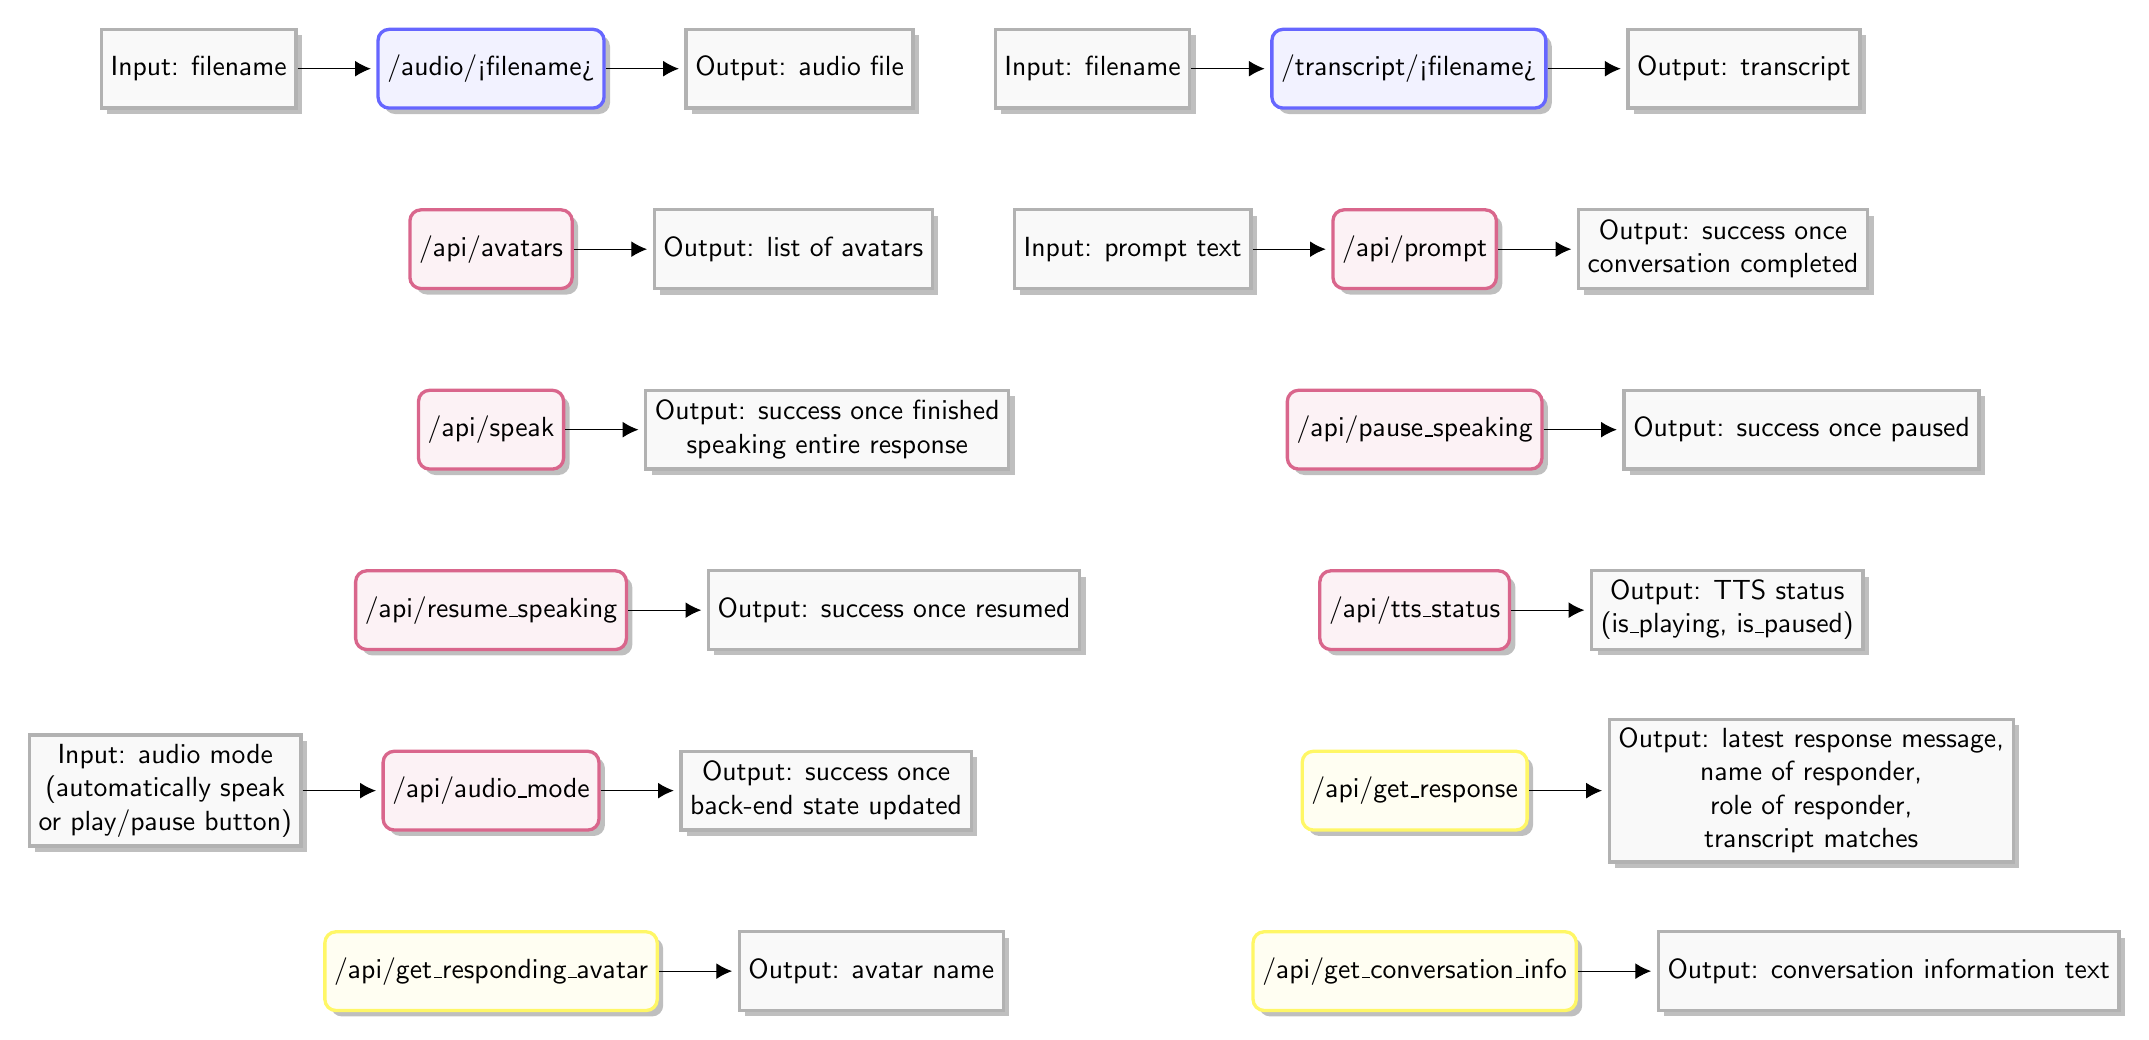
\begin{tikzpicture}[
                node distance=1.25cm and 1cm,
                every node/.style={fill=white, font=\sffamily, drop shadow},
                align=center,
                >={Latex[width=2mm,length=2mm]},
                io/.style={rectangle, draw=gray!60, fill=gray!5, very thick, minimum height=10mm},
                podcast/.style={rectangle, draw=blue!60, fill=blue!5, very thick, minimum height=10mm, rounded corners},
                avatar/.style={rectangle, draw=purple!60, fill=purple!5, very thick, minimum height=10mm, rounded corners},
                polling/.style={rectangle, draw=yellow!60, fill=yellow!5, very thick, minimum height=10mm, rounded corners},
                line/.style={draw, ->, shorten >=2pt},
                ]
        
                % Place nodes in two columns
                \node [podcast] (audio) {/audio/<filename>};
                \node [io, left=of audio] (inputAudio) {Input: filename};
                \node [io, right=of audio] (outputAudio) {Output: audio file};
                \node [io, right=of outputAudio] (inputTranscript) {Input: filename};
                \node [podcast, right=of inputTranscript] (transcript) {/transcript/<filename>};
                \node [avatar, below=of audio] (avatars) {/api/avatars};
                \node [io, right=of avatars] (outputAvatars) {Output: list of avatars};
                \node [io, right=of outputAvatars] (inputPrompt) {Input: prompt text};
                \node [avatar, right=of inputPrompt] (prompt) {/api/prompt};
                \node [avatar, below=of avatars] (speak) {/api/speak};
                \node [avatar, below=of prompt] (pause) {/api/pause\_speaking};
                \node [avatar, below=of speak] (resume) {/api/resume\_speaking};
                \node [avatar, below=of pause] (status) {/api/tts\_status};
                \node [avatar, below=of resume] (mode) {/api/audio\_mode};
                \node [polling, below=of status] (response) {/api/get\_response};
                \node [polling, below=of mode] (responding) {/api/get\_responding\_avatar};
                \node [polling, below=of response] (conversation) {/api/get\_conversation\_info};
        
                % Define input and output nodes for each API endpoint
                \node [io, right=of transcript] (outputTranscript) {Output: transcript};
        
                \node [io, right=of prompt] (outputPrompt) {Output: success once\\ conversation completed};
        
                \node [io, right=of speak] (outputSpeak) {Output: success once finished\\ speaking entire response};
        
                \node [io, right=of pause] (outputPause) {Output: success once paused};
        
                \node [io, right=of resume] (outputResume) {Output: success once resumed};
        
                \node [io, right=of status] (outputStatus) {Output: TTS status \\ (is\_playing, is\_paused)};
        
                \node [io, left=of mode] (inputMode) {Input: audio mode \\(automatically speak\\ or play/pause button) };
                \node [io, right=of mode] (outputMode) {Output: success once \\back-end state updated};
        
                \node [io, right=of response] (outputResponse) {Output: latest response message,\\ name of responder, \\role of responder, \\transcript matches};
        
                \node [io, right=of responding] (outputResponding) {Output: avatar name};
        
                \node [io, right=of conversation] (outputConversation) {Output: conversation information text};
        
                % Draw arrows from inputs to nodes and nodes to outputs
                \draw[line] (inputAudio) -- (audio);
                \draw[line] (audio) -- (outputAudio);
        
                \draw[line] (inputTranscript) -- (transcript);
                \draw[line] (transcript) -- (outputTranscript);
        
                \draw[line] (avatars) -- (outputAvatars);
        
                \draw[line] (inputPrompt) -- (prompt);
                \draw[line] (prompt) -- (outputPrompt);
        
                \draw[line] (speak) -- (outputSpeak);
        
                \draw[line] (pause) -- (outputPause);
        
                \draw[line] (resume) -- (outputResume);
        
                \draw[line] (status) -- (outputStatus);
        
                \draw[line] (inputMode) -- (mode);
                \draw[line] (mode) -- (outputMode);
        
                \draw[line] (response) -- (outputResponse);
        
                \draw[line] (responding) -- (outputResponding);
        
                \draw[line] (conversation) -- (outputConversation);
        
            \end{tikzpicture}}
            \caption{A high-level overview of the Flask server routes and their inputs and outputs. Blue routes relate to podcast content delivery to the front-end, red routes correspond to interaction with conversational avatars, and yellow routes involve polling the back-end state. Note that the inputs flow from the front-end to the back-end, and the outputs flow in the opposite direction.}
            \label{fig:flaskroutes}
        \end{figure}
        
        \subsection{Conversation Management}
        \indent Once prompts are received from the front-end, they are routed to the relevant avatar as decided by the \texttt{ConversationManager} class. This decision is made dynamically, based upon the content of the user prompt itself rather than any explicit commands.
        
        \subsubsection{Conversation Types}
        \indent Users can engage in five conversation types with the conversational avatars consisting of two main modalities and three other interaction types: 

        \begin{itemize}
            \item \textbf{Solo Conversation}: This conversation type pertains to a direct one-on-one conversation with a singular avatar and the user. These prompts can be directed at any human-based avatar or AIden. The user directs their prompt to this avatar either by clicking on its icon and using the speech recognition functionality or by mentioning its name (or a common variation or nickname of its name) in their prompt.
            \item \textbf{Multi-Avatar Discussion}: A discussion between available conversational avatars gleaned from the user's prompt. The discussion is essentially a back-and-forth dialogue where avatars respond one at a time to each other. The user can specify who they want to participate in the discussion by naming them in their prompt. At the end of the discussion, the first speaker wraps it up and thanks the user for their question.
            \item \textbf{Undirected Conversation}: This case occurs when the user does not name anyone in their prompt. In this case, the system determines who should respond. This conversation mode can trigger either a solo conversation or a discussion. 
            \item \textbf{AI Assistant Intervention}: If the answer to the user's prompt cannot be found within the transcript, the system evaluates the nature of the prompt to determine if it requires AI intervention. An intervention can happen in these cases:
                \begin{itemize}
                    \item The prompt may lead to a response that promotes hate or violence.
                    \item The prompt may lead to a response that contains misinformation.
                    \item The prompt may lead to a response that is not characteristic of the avatar it's directed to.
                \end{itemize} 
            When one of these scenarios happens, intervention means the human-based avatar does not have to answer such prompts and risk generating something in an actual human's voice that may lead to real harm in that person's life. This intervention seeks to address design goal \textbf{D5}.
            \item \textbf{Human Avatar Intervention}: This is similar to the AI assistant intervening. However, this case occurs if the prompt seems to have been directed to an avatar by mistake when it should have been directed to a different avatar. This conversation type allows for a greater sense of realism, as avatars will only attempt to answer based on the real-life abilities of their reference. 
        \end{itemize}
        
        \subsubsection{Conversation Manager}
        \indent Upon receiving a user prompt, an instance of the \texttt{ConversationManager} class is initialized, and the prompt is passed through a routing method. The \texttt{ConversationManager} class was designed to ensure conversations are routed and managed to reflect the context of user prompts, a principle central to design goal \textbf{D4}: Optimize for Contextual Understanding. This goal is achieved by using calls to GPT-4 Turbo, separate from those for the avatar conversations, to interpret listener prompts and determine the most appropriate conversation dynamics.
        
        \indent When a prompt is received, the \texttt{ConversationManager} performs several steps to determine the nature of the response required: 
        \begin{enumerate}
            \item \textbf{Prompt Analysis}: The LLM is consulted to analyze the user prompt in conjunction with the transcript. This analysis is facilitated through a specific query, which can be seen in \ref{table:conversationprompts} in Appendix \ref{app:G}. The query includes the user's prompt and the transcript alongside a list of available avatar names. The purpose here is to decipher primary and secondary participants from the avatars based on the prompt's direct mentions and contextual cues.
            \item{LLM Response Interpretation}: The response from the LLM is expected in a structured JSON format, detailing critical aspects like the primary avatar targeted by the prompt, any secondary avatars who should be involved in a potential discussion or who would be better suited to answer the prompt than the primary avatar, and flags for discussions, AI interventions, or if the target speaker in the user prompt should not be the one to respond. If there is no speaker directly identified in the user prompt, it is here that the \texttt{ConversationManager} determines who should respond. This structured response allows for precise action to be taken in subsequent steps.
            \item \textbf{Conversation Routing}: Depending on the JSON output from the LLM, there are several courses of action:
            \begin{enumerate}
                \item \textbf{AI Intervention:} The flag relating to AI intervention is checked first since this precludes any other type of conversation. If an intervention is meant to occur, the prompt is sent to another method, with the primary avatar apologizing for being unable to answer, followed by AIden's response.
                \item \textbf{Human Avatar Intervention:} Next, the flag for whether the primary speaker should respond is checked. If this flag is false, the primary avatar apologizes for being unable to answer and states that the other avatar(s) identified would be a better respondent. Then, the other avatar(s) responds to the user prompt as either a discussion or a solo response. 
                \item \textbf{Discussion Initiation:} If the prompt is found to suggest a discussion involving multiple avatars, a discussion session is initiated. The JSON output of the LLM call should contain a list of discussion participants. This list is sent to another method where the avatars interact in a dialogue managed by another LLM routine, the Discussion Arbiter.
                \item \textbf{Solo Response:} Finally, if a primary avatar is identified in the prompt and is an existing avatar, and no discussion is necessary, the conversation is routed directly to this avatar to respond. 
                \item \textbf{Undetermined:} If the primary avatar identified does not exist or any other errors are encountered during this process, AIden responds by saying that the desired avatar could not be determined and to restate the prompt.
            \end{enumerate}
            \item \textbf{Conversation Information Updated}: Now that the conversation type has been inferred, the conversation information global variable is set to text that lists what type of conversation will occur and which avatar(s) will be responding to the prompt. This text is then displayed in the chat room in the Chat History component of the user interface.
            \item \textbf{Individual Avatars Handle Response}: Following, the avatars handle their own LLM queries. The first thing that happens is that a global variable is set that shows which is currently responding. This message pulses in the front-end while waiting for the response from the LLM. If the speak mode has been set in the front-end such that the avatar should automatically speak, it is here that the TTS is played once the response is received from the GPT-4 Turbo API. 
            \item \textbf{Transcript Matching}: Following this, the prompt is compared against the transcript to see if it matches any part of the transcript. Once again, this is meant to provide a sense of authenticity to the responses as required by design goal 
            textbf{D2}. All matches are added to a list alongside their similarity score. If no matches are found, the list is simply empty.
            \item \textbf{Update Latest Response Global}: Lastly, once the avatar response has been compared to the transcript, the global variable corresponding to the latest response is updated. The front-end polls for this value, so once it's changed, the front-end publishes the new avatar response.
            \item \textbf{Await New Prompt}: Now, the Flask server waits for a new user prompt after the conversation is complete.
        \end{enumerate}

        A detailed pipeline diagram of the conversation management setup is shown in Figure \ref{fig:conversationmanager}.

        \begin{figure}[H]
            \centering
            \noindent\resizebox{\textwidth}{!}{%
            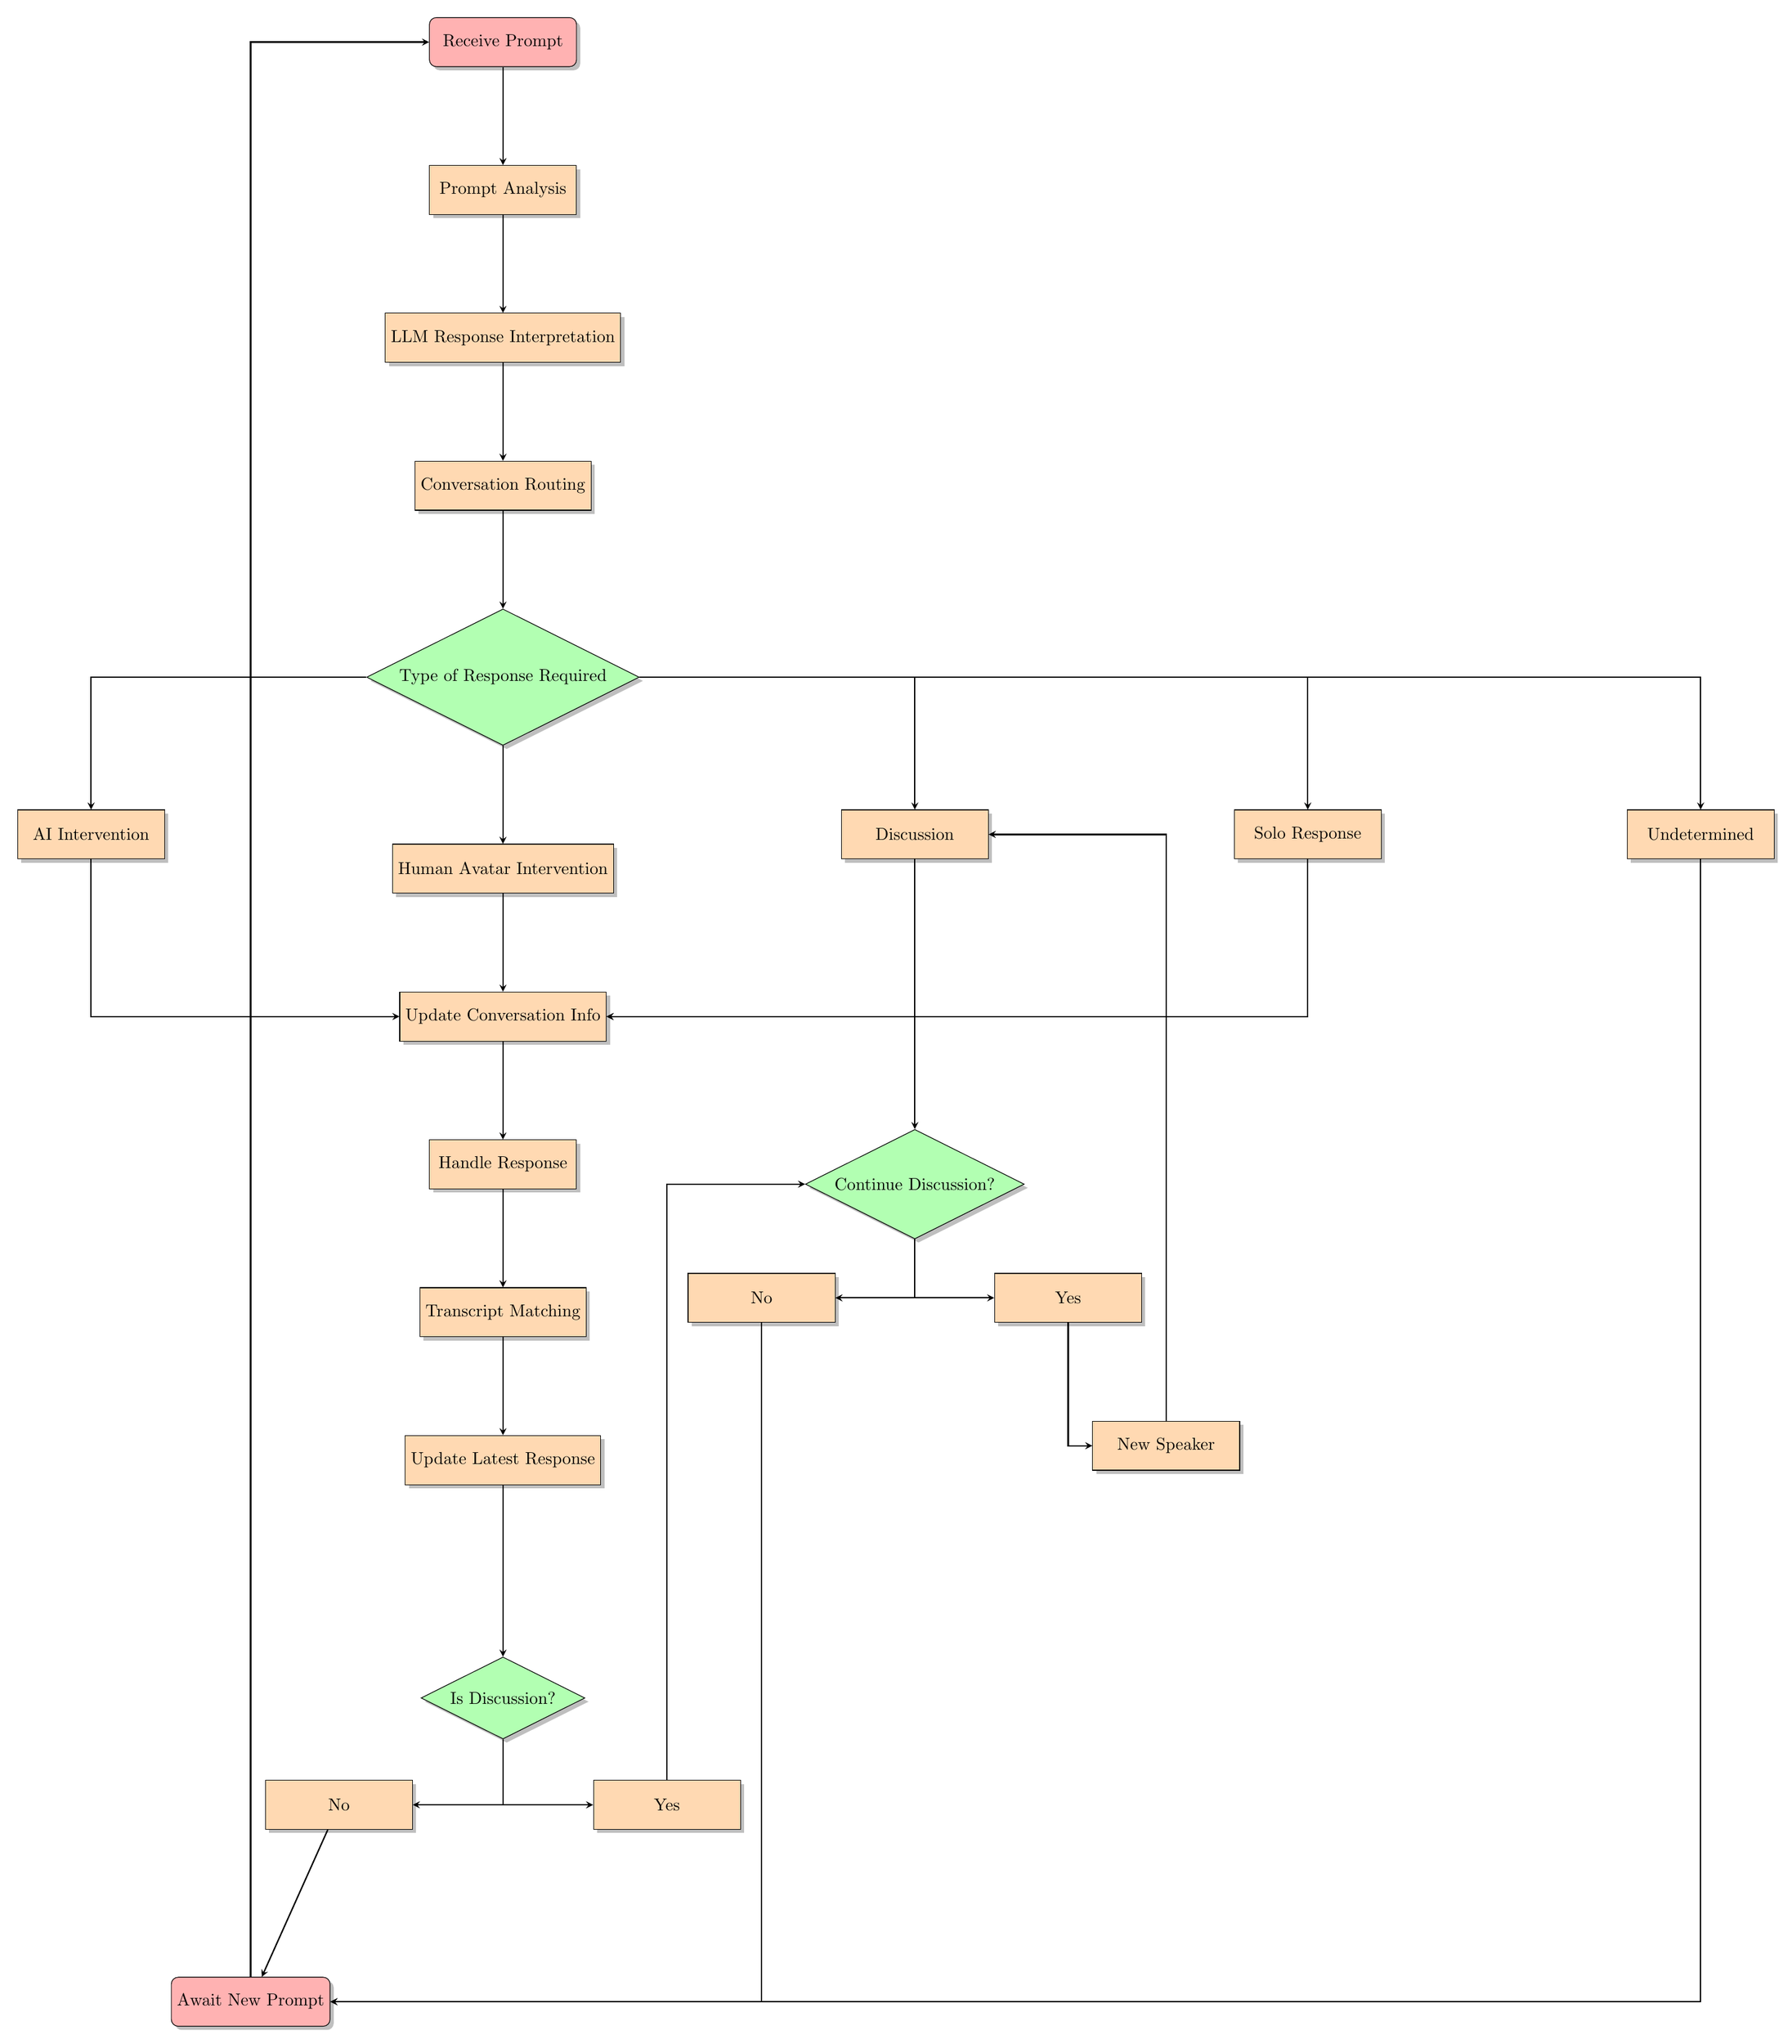
\begin{tikzpicture}[node distance=2cm and 2.5cm, auto]
                % Styles
                \tikzset{every node/.style={drop shadow}}
                \tikzstyle{startstop} = [rectangle, rounded corners, minimum width=3cm, minimum height=1cm, text centered, draw=black, fill=red!30]
                \tikzstyle{process} = [rectangle, minimum width=3cm, minimum height=1cm, text centered, draw=black, fill=orange!30]
                \tikzstyle{decision} = [diamond, aspect=2, text centered, draw=black, fill=green!30]
                \tikzstyle{arrow} = [thick,->,>=stealth]
        
                % Nodes
                \node (init) [startstop] {Receive Prompt};
                \node (analyze) [process, below=of init] {Prompt Analysis};
                \node (interpret) [process, below=of analyze] {LLM Response Interpretation};
                \node (route) [process, below=of interpret] {Conversation Routing};
                \node (decision) [decision, below=of route] {Type of Response Required};
                \node (ai) [process, below left=of decision, xshift=-3cm] {AI Intervention};
                \node (human) [process, below=of decision] {Human Avatar Intervention};
                \node (discussion) [process, below right=of decision, xshift=3cm] {Discussion};
                \node (arbiter) [decision, below =of discussion, yshift=-3.5cm] {Continue Discussion?};
                \node (yes) [process, below right=of arbiter, xshift=-2cm, yshift=0.75cm] {Yes};
                \node (new) [process, below = of yes, xshift=2cm] {New Speaker};
                \node (no) [process, below left=of arbiter, xshift=2cm, yshift=0.75cm] {No};
                \node (solo) [process, right=of discussion, xshift=2.5cm] {Solo Response};
                \node (undetermined) [process, right=of solo, xshift=2.5cm] {Undetermined};
                \node (update) [process, below=of human] {Update Conversation Info};
                \node (response) [process, below=of update] {Handle Response};
                \node (match) [process, below=of response] {Transcript Matching};
                \node (update2) [process, below=of match] {Update Latest Response};
                \node (discuss) [decision, below =of update2, yshift=-1.5cm] {Is Discussion?};
                \node (yes2) [process, below right=of discuss, xshift=-1.5cm, yshift=0.75cm] {Yes};
                \node (no2) [process, below left=of discuss, xshift=1.5cm, yshift=0.75cm] {No};
                \node (wait) [startstop, below=of no2, yshift=-1cm, xshift=-1.8cm] {Await New Prompt};
        
                % Paths
                \draw [arrow] (init) -- (analyze);
                \draw [arrow] (analyze) -- (interpret);
                \draw [arrow] (interpret) -- (route);
                \draw [arrow] (route) -- (decision);
                \draw [arrow] (decision) -| (ai);
                \draw [arrow] (decision) -- (human);
                \draw [arrow] (decision) -| (discussion);
                \draw [arrow] (decision) -| (solo);
                \draw [arrow] (decision) -| (undetermined);
                \draw [arrow] (ai) |- (update);
                \draw [arrow] (human) -- (update);
                \draw [arrow] (discussion) -- (arbiter);
                \draw [arrow] (discussion) |- (update);
                \draw [arrow] (arbiter) |- (yes);
                \draw [arrow] (arbiter) |- (no);
                \draw [arrow] (yes) |- (new);
                \draw [arrow] (new) |- (discussion);
                \draw [arrow] (no) |- (wait);
                \draw [arrow] (solo) |- (update);
                \draw [arrow] (undetermined) |- (wait);
                \draw [arrow] (update) -- (response);
                \draw [arrow] (response) -- (match);
                \draw [arrow] (match) -- (update2);
                \draw [arrow] (update2) -- (discuss);
                \draw [arrow] (discuss) |- (yes2);
                \draw [arrow] (discuss) |- (no2);
                \draw [arrow] (no2) -- (wait);
                \draw [arrow] (yes2) |- (arbiter);
                \draw [arrow] (wait) |- (init);
        
            \end{tikzpicture}}
            \caption{Pipeline diagram of the Conversation Management System}
            \label{fig:conversationmanager}
        \end{figure}

        \subsubsection{Discussion Arbiter}
        \indent The Discussion Arbiter is not a separate class; it simply describes another LLM query set-up that allows for the discussion to be dynamically monitored as it progresses. In the method that handles the discussion, the primary speaker introduces the discussion topic based on the user prompt and the other avatars who will be responding, asking them for their thoughts. Following this, the Discussion Arbiter evaluates who should speak next in a loop that iterates after completing a single response. This decision is based on a dynamic understanding of the ongoing conversation, the relevance of each avatar's potential input, and the natural flow of dialogue. The Arbiter also assesses whether the conversation has reached a natural conclusion. The Discussion Arbiter determines whether additional responses add value or if the dialogue has satisfactorily addressed the user's query. The LLM query used to determine these discussion management factors can be seen in \ref{table:conversationprompts} in Appendix \ref{app:G}. Thus, the Discussion Arbiter dynamically adjusts who should speak next and when to end the conversation based on real-time updates to the dialogue, ensuring that the discussion remains engaging and on-topic and adhering to the original user prompt and overall context provided by the podcast transcript.
        
        \subsubsection{Transcript Referencing}
        \indent The code to match each avatar response to the transcript is structured around two primary tasks: prioritizing sentences that contain named entities and measuring the similarity between sentences to identify matches.
        
        \paragraph{Named Entity Recognition (NER)} The code employs the SpaCy library with the en\_core\_web\_sm model to identify entities like persons, organizations, and locations \citep{spacy}. NER is crucial for extracting significant information from texts. These techniques make it easier to find transcript matches by simply finding parts of the transcript that include the same or similar entities to those in response \citep{mohit2014named}.
        
        \paragraph{Sentence Similarity Calculation} To measure how closely sentences are related semantically, the code uses the SentenceTransformer library, specifically the all-MiniLM-L6-v2 model \citep{reimers2019sentence}. This model creates sentence embeddings and uses cosine similarity to assess their similarity. Cosine similarity is widely used in semantic analysis as it efficiently determines similarity in vector space, reflecting the semantic proximity between sentences, allowing for more accurate transcript matches \citep{reimers2019sentence}.\\

        \indent The transcript analysis module integrates these two tasks by first segmenting and prioritizing sentences from a response and the podcast transcript based on their content and named entities. It then computes embeddings for these sentences and finds the best match based on the highest cosine similarity score, considering only those matches that exceed a similarity threshold tuned during testing (0.6 in this case).
        
        \indent An example output of the matching logic is shown in Table \ref{table:transcriptmatches}. Since this similarity score is above the threshold, it would be accepted as a valid match.

        \begin{table*}[h]
            \caption{Example transcript match.}
            \label{table:transcriptmatches}
            \centering
            \resizebox{\textwidth}{!}{
            \begin{tabular}{ >{\raggedright\arraybackslash}p{2cm} | >{\raggedright\arraybackslash}p{4cm} | >{\raggedright\arraybackslash}p{4cm} | >{\raggedright\arraybackslash}p{3.8cm} }
                \toprule
        \textbf{Prompt}  
        &\textbf{Response}      
        & \textbf{Transcript Match}   
        & \textbf{Similarity Score} 
        \\\midrule
        Ira, where is the clinic in the episode?
        & Umm, the clinic is located in North Carolina, a place called Cane Creek, about 15 miles outside of Asheville.
        &  'And there was this one job that he was really excited about at a small rural clinic in North Carolina, a place called Cane Creek, about 15 miles outside of Asheville.'
        & 65.4\%\\
                \bottomrule
            \end{tabular}
        }
        \end{table*}

        \clearpage

        \chapter{User Evaluation}
        A qualitative user study was conducted to validate that \textit{ReciproCast} meets the design goals. This study aimed to understand if such a system improved the podcast listening experience in a meaningful way, determine the effects of interactivity on listener engagement and enjoyment, and garner feedback on ways that the system, in its current implementation, could be improved.
        
        \section{Participants}
        Six participants were selected for the study of varying educational backgrounds. We thought this was important because we wanted to see how people less familiar with how LLMs work or less attuned to the current state of research as those more familiar with the limitations of such models engage with the system. Thus, each participant provided a broader range of usage examples that may better reflect the diversity of podcast listeners. Additionally, we reached out to participants of the formative interviews, and two of them (P01 and P04) could participate. Doing so allowed for the evaluation of how the design met user expectations. Their participation acted as a litmus test to see if what we built was actually informed by the formative interviews, validating the design goals, the design space, and the design itself. We also interviewed two podcast creators (P04 and P05). This allowed us to gauge whether or not a system like \textit{ReciproCast} would be helpful for creators as well as listeners and gain insight into what would enhance its utility for both demographics. The demographic data of the user study participants is summarized in Figure \ref{fig:userdemographics}.
        
        \begin{figure}[H]
        \centering
          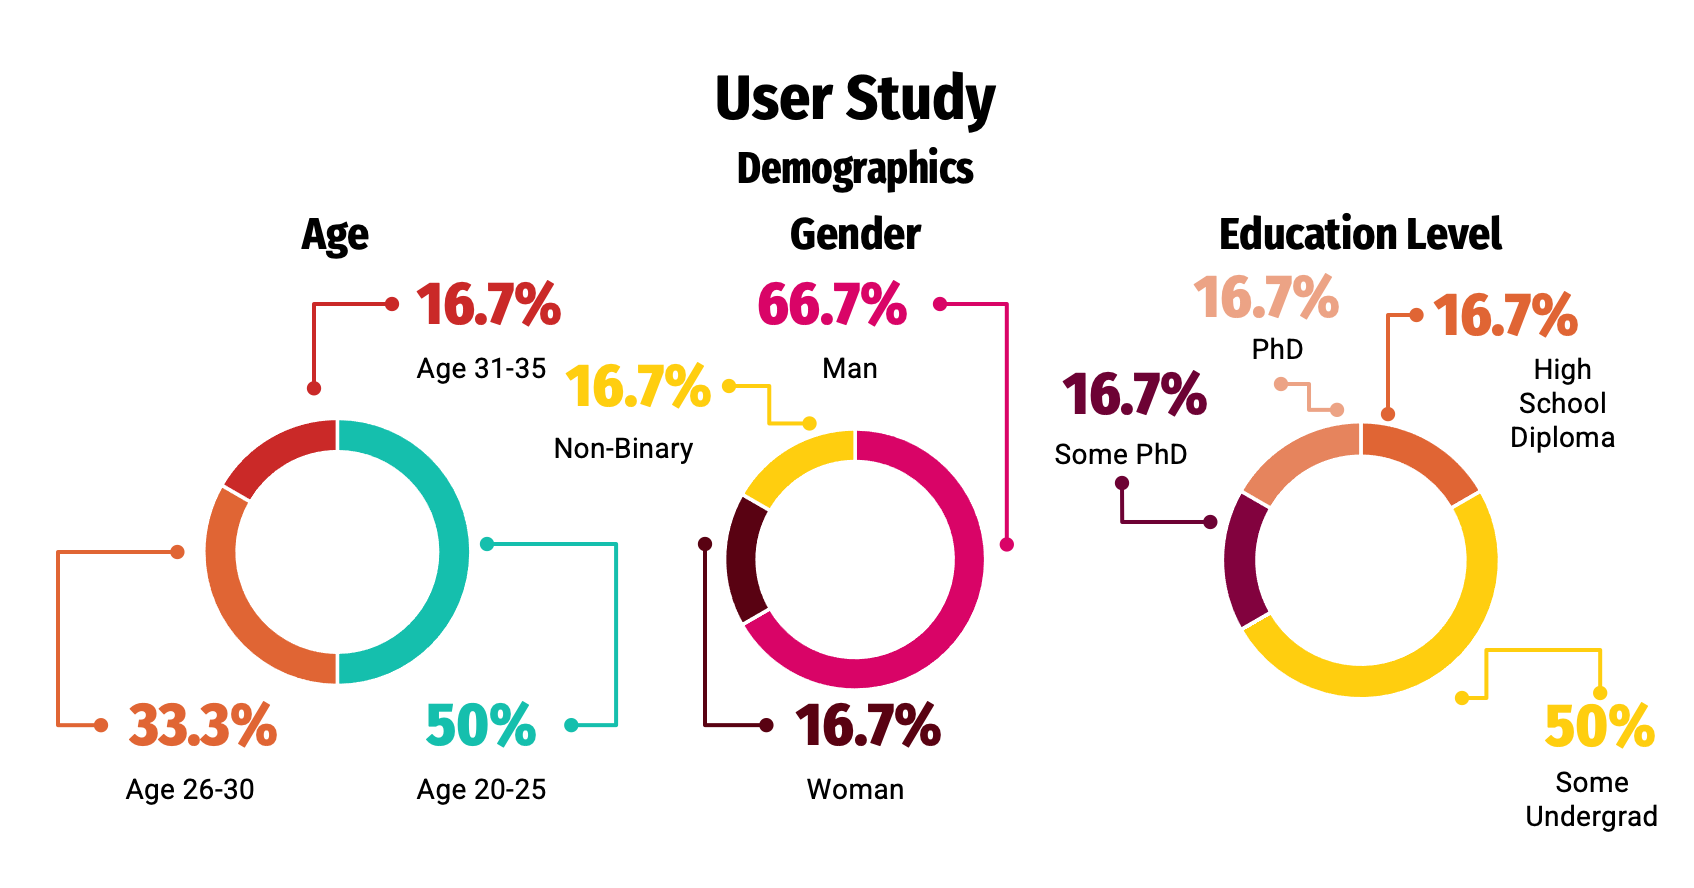
\includegraphics[width=1\textwidth]{figures/userstudydemog.png}
          \caption{Demographic information collected in the user study survey, including the age, gender identity, and education level of participants.}
          \label{fig:userdemographics}
        \end{figure}

        Lastly, participants were also asked about their experience with podcasts (both listening and creating) and their listening habits. This ensured that the participants were the project's target stakeholders, providing validity to their insights as representatives of \textit{ReciproCast's} target demographic. Additionally, learning about what types of podcasts they listen to, the environments they listen to podcasts in, and their purposes for listening to podcasts allowed for a better explanation of their reasoning for engaging with specific features in particular ways or their preferences towards certain design aspects. The responses by each participant are broken down in Table \ref{table:userhabits}.

        {\small \begin{longtable}{ 
                >{\raggedright\arraybackslash}p{0.04\linewidth} |  
                >{\raggedright\arraybackslash}p{0.1\linewidth} | 
                >{\raggedright\arraybackslash}p{0.11\linewidth}  |
                >{\raggedright\arraybackslash}p{0.15\linewidth} |
                >{\raggedright\arraybackslash}p{0.17\linewidth} |
                >{\raggedright\arraybackslash}p{0.125\linewidth} |
                >{\raggedright\arraybackslash}p{0.19\linewidth}
            }
            \caption{User study participant information and listening habits}
            \label{table:userhabits}\\
            \toprule    
            \textbf{ID}   
            & \textbf{Creator or listener?}
            & \textbf{How long?}
            & \textbf{What platform(s) do you use?}
            & \textbf{Where do you listen to podcasts?}
            & \textbf{Informative or entertaining?}
            & \textbf{What is the purpose for listening?}
            \\ 
            \midrule
            \endfirsthead
            
            \multicolumn{7}{c}%
            {{\bfseries \tablename\ \thetable{} -- continued from previous page}} \\
            \toprule    
            \textbf{ID}   
            & \textbf{Creator or listener?}
            & \textbf{How long?}
            & \textbf{What platform(s) do you use?}
            & \textbf{Where do you listen to podcasts?}
            & \textbf{Informative or entertaining?}
            & \textbf{What is the purpose for listening?}
            \\ 
            \midrule
            \endhead
            P01
            & Listener
            & 5+ Years
            & Spotify, Google Podcasts
            & While walking, While taking public transit
            & Informative
            & To learn about something or some event, To stay updated with current events, To have something to listen to while I work, To practice another language \\
            \midrule
            P02
            & Listener
            & 1 - 2 Years
            & Youtube Music
            & At home, At work, While walking, While doing chores
            & A mixture of both
            & To be entertained, To stay updated with current events, To have something to listen to while I work \\
            \midrule
            P03
            & Listener
            & 5+ Years
            & Apple Podcasts, YouTube
            & While driving, While walking, While taking public transit, While working out, While shopping, While doing chores
            & Informative
            & To learn about something or some event, To stay updated with current events, To have something to listen to while I work, To practice another language \\
            \midrule
            P04
            & Both
            & 5+ Years
            & Spotify, Apple Podcasts, Google Podcasts, Youtube Music, iHeartRadio
            & At home, While driving, At work, While walking, While working out, While shopping, While doing chores
            & Entertaining
            & To be entertained, To have something to listen to while I work\\
            \midrule
            P05
            & Both
            & 5+ Years
            & Spotify
            & At work, While walking, While taking public transit, While doing chores
            & A mixture of both
            & To learn about something or some event, To be entertained, To have something to listen to while I work \\
            \midrule
            P06
            & Listener
            & 3 - 4 Years
            & Spotify
            & At home, While driving, At work, While walking, At school, While doing chores, shower
            & A mixture of both
            & To be about something or some event, To be entertained, To have something to listen to while I work, to spook myself \\
            \bottomrule
        \end{longtable}}

        
        \section{Study Protocol}
        The user study was conducted in person and online to allow users from different countries and provinces to participate. The remote sessions took place on Zoom, and users controlled the system via screen-sharing. In both cases, \textit{ReciproCast} ran on a ROG-STRIX SCAR laptop with an RTX 2070 Super graphics card.
        
        These user primitives informed the development of the study protocol:

        \begin{itemize}
            \item \textbf{User listens to podcast}: This includes interacting with the scrub bar and transcript, simulating the current passive listening experience.
            \item \textbf{Text box prompting}: This primitive involves typing prompts into the text box and hitting enter to send the message to the back-end.
            \item \textbf{Audio-based prompting}: This can happen by clicking on the avatar icon you want to speak to or by clicking the microphone button.
            \item \textbf{Mixed prompting}: The user starts with an audio prompt and then edits it in the text box.
            \item \textbf{In-context discussion}: This type of discussion consists of prompts that can be answered directly from the podcast transcript. In this case, the avatar uses information from the transcript to respond, and the text response should have accurate transcript matches. When the user clicks these match links, the podcast playback should skip to the relevant part.
            \item \textbf{Out-of-context discussion}: Prompts in this type of discussion will solicit new information from the LLM that is not extractable from the episode.
        \end{itemize}

        A protocol was developed in which participants were walked through examples of these primitives, including the different types of possible conversation. Following this, users were allowed to engage with the system through a structured task. The task involved using the system to listen to and interact with a podcast via the various prompting methods outlined. Each study used a different podcast to test the system's robustness across other content types. This approach helped confirm that the system performed consistently regardless of the specific podcast content. For P04's study, his own podcast was used, providing a personal insight into the authenticity of the avatars for that podcast in terms of their voices and how they respond. Participants were encouraged to think aloud during the task, providing real-time feedback and commentary on their experience and any difficulties encountered. This process was designed to simulate a natural interaction with the system and to gather insights into user behaviours and preferences.
        
        \indent After the task, participants completed a detailed survey designed to assess their overall satisfaction with the experience, the usability of the system, and the effectiveness of the interaction modes provided. The survey included questions about the ease of use of the interface, the clarity of the avatar responses, and the relevance of the information provided by the avatars. It allowed for the collection of more quantitative data to back up the qualitative results from the post-study interview. The interviews lasted anywhere from 20-30 minutes and were semi-structured, with some prepared questions and room for following up on participant responses. Participants were encouraged to discuss their survey responses and provide additional qualitative feedback and feature ideas. The interviews focused on aspects such as the usefulness of the different types of avatar interactions, the alignment of avatar voices with their expectations, and any suggestions for improving the system. Participants were also asked about their willingness to use such a system in the future and to consider potential alternative applications for the technology.

        \indent Participants were asked to fill out a consent form (as shown in \ref{app:L}) and were compensated \$25 CAD. Each study lasted no longer than 90 minutes. The link in Appendix \ref{app:I} shows the details and script of the user study protocol.
        
        \section{Results and Findings}
        In the user study, the use of \textit{ReciproCast} showcased several thematic areas that highlight the system's influence on podcast interaction, aligning closely with the anticipations outlined in the formative interviews and refined through the design space conceptualization. Additional plots of the quantitative results from the survey are located in Appendix \ref{app:I}.

        \subsection{Engagement \& Novelty}
        Participants generally reported high levels of engagement due to the novel interaction possibilities offered by \textit{ReciproCast}. They appreciated the ability to engage directly with podcast content through real-time questioning and receiving immediate responses from conversational avatars. Multiple participants expressed that this type of interaction was not possible with the current status quo of podcast consumption. For example, P03 highlighted the immersive nature of the interaction, stating, “I’m not a passive listener anymore. In some way, I’m a part of the conversation." This sentiment further emphasizes the existence of the gap shown in Figure \ref{fig:interaction}. This sentiment was echoed across the board, with the system's novelty rated highly (Mean: 9/10, STD: 1.67), suggesting a uniform appreciation for this feature across participants. Specifically, the users agreed that it was how \textit{ReciproCast} allows users to engage with podcasts that makes it so novel (Mean: 4.8/5, STD: 0.41). 

        \indent Participants found the real-time questioning feature transformative, allowing them to actively delve deeper into podcast topics. P02, P03, and P04 each described a frustration. When they miss something when regularly listening to podcasts, the only way to get clarification is by moving off the podcast platform to search for an answer or simply ignoring the missed information. The users generally found the \textit{ReciproCast} system more approachable and convenient. P04's experience exemplifies this, stating that the ability to query podcast avatars directly made the content more engaging. This insight aligns with research into podcast engagement factors as the system allows for a more participatory experience \citep{GarciaMarin2020}. This theme is also statistically supported by a high level of agreement that \textit{ReciproCast} helped them stay engaged in the podcast episode (Mean: 4/5, STD dev: 0.89).

        \subsection{Multi-Modal Capabilities}
        Interestingly, while speech-based Q\&A was preferred in formative interviews, text-based interaction was widely preferred by the user study participants. P01 and P03 ranked it as their least favourite way of interacting with the avatars, while P04 and P05 did not engage with it. Text-based prompting was much more popular, with all 6 participants ranking it higher. There were several reasons for this. The most obvious was because most of the studies were run remotely over Zoom, thus interfering with the ability of the microphone to pick up the participants' voices. 
        
        \indent Additionally, in the in-person studies, users expressed that since the study was run on a laptop in a quiet setting, it was much easier to type the prompt rather than rely on speech recognition, which was not always accurate. Those who ranked the feature higher, like P05, and rated it second highest stated that they would undoubtedly use the voice prompting feature in a different environment, like while doing chores or exercising, supporting claims from the formative interviews. One idea for improvement in this area that P05 brought up was using a wake word to start speech recognition rather than having to click manually.
        
        \indent However, users did appreciate the perceived ability to control the level of interruption of the TTS. The ability to automatically have the audio play vs pressing the play button allowed users to specify how and when they wanted text to be read to them. Both P05 and P06 enjoyed using the automatic playback mode, especially for the discussion conversation type, with the former stating it was convenient not to look at the Chat History pane while listening. In general, users agreed that using \textit{ReciproCast} did not take away from their listening experience (Mean: 8.3/10, STD: 2.25) and that the features of \textit{ReciproCast} were such that using the system was not too distracting from the podcast content (Mean: 8.3, STD: 1.4). Thus, while multi-modal support in terms of prompting received mixed reviews, the participants appreciated the ability to have the avatar responses be spoken to them or just presented in textual form. These results show that \textit{ReciproCast} is at least partially successful at fulfilling design goal \textbf{D1}.

        \subsection{Realism \& Authenticity}
        The realism of the synthesized voices and the authenticity of the avatar responses were critical in how participants connected with the content. First, the believability of the responses provided by the avatars varied among participants. P01 and P06 rated their believability high (8/10 and 9/10, respectively), noting that the responses felt contextually appropriate, cohesive, and well-integrated into the podcast dialogue. P06 specifically enjoyed the banter between the avatars in discussions, stating, “It felt like I was talking to a panel, like I was in the room with them.” P02 agreed with this sentiment, praising the response quality in facilitating an interaction that felt like conversing with a real person. P05 was a little more on the fence, stating that the responses were generally believable, but some of the quips made by the avatars felt repetitive or forced. P04 was more critical, noting that while responses were entertaining, the language used was still stiff. Since his own podcast was used for his study, his insights into the realism of the responses were crucial. He stated that while responses were factually accurate to the podcast content, their expression was far more rigid than natural. The models would need more tuning and potentially access to more of the speaker's content to "pick up the nuances in speech patterns." In general, however, the participants found the responses' realism to be acceptable (Mean: 6.8/10, STD: 1.7). 

        \indent This score was also influenced by the quality of the synthesized voices, with users like P03 citing it as the main reason he found the responses less believable. This feature received mixed reactions. Some participants, like P01, P05, and P06, appreciated the voices for adding a layer of personalization and authenticity to the avatars, making them feel more connected to the people in the podcast. P06 stated, "The voices sounded quite natural, which helped me connect with the content more." P03 and P04 were the most critical of the synthesized voices, giving them a rating of 3/10 and 4/10, respectively. The most common complaint about the voices was not that they did not match the tone or timbre of the speaker; this was generally praised (particularly by P02 and P03), but the playback speed of the speech was relatively slow, and the speaker would take several unnatural pauses and breaths. Sometimes, the speaker would take on a British-sounding accent. This odd behaviour occurred in P05's study and is likely due to the data used to train the XTTS model \citep{XTTS_Coqui}. A common theme amongst participants was that the quality of the TTS of the human-based avatars was a limiting factor for realism and that better models would improve the quality of the interaction. P01 stated that because the voices were slightly off, it drew attention from the response's content because the imperfections made her feel the need to scrutinize the voice quality. In contrast, users generally praised AIden's voice. 
        
        \indent While this quality was a significant point of dissatisfaction, most users, including P05 and P06, believed the feature was essential to the system. P05 argued that the synthesized voices were one of the main factors supporting the system's novelty. P06 claimed that having voices serves as an essential accessibility feature. They argued from their own experience that having voices that mimicked the voices in the podcast is helpful for those with attention disorders to stay engaged and that having TTS as a feature, in general, is essential for those with visual impairments. Thus, due to their controversial reception, the synthesized voices were one of the lower-rated features of \textit{ReciproCast}, achieving a neutral score indicative of the divergent opinions of participants (Mean: 5.7/10, STD: 2.1). 

        \begin{figure}[H]
        \centering
          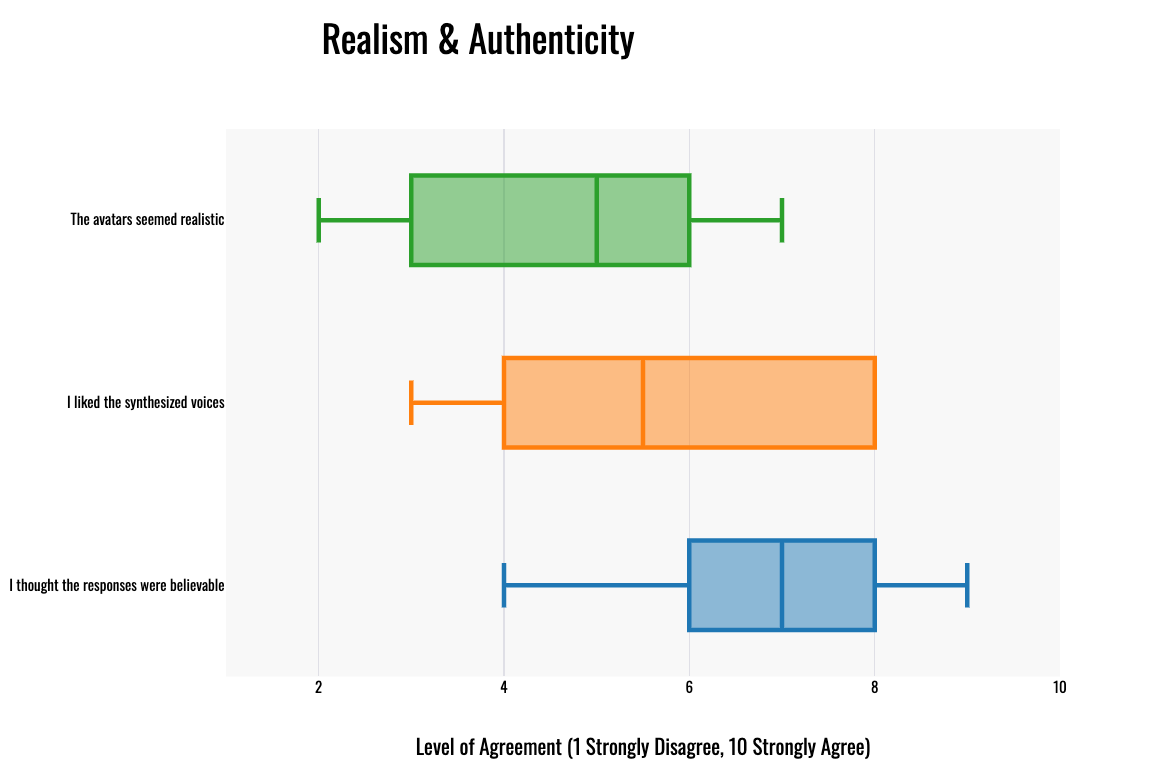
\includegraphics[width=1\textwidth]{figures/realism.png}
          \caption{Box and whisker plot showing user agreement with statements on avatar and response realism and authenticity.}
          \label{fig:realism}
        \end{figure}

        \indent Therefore, due to the speech synthesis receiving more mixed reviews, the system's realism is the largest area of improvement. On average, participants rated the realism of the avatars as a whole at 4.7/10 with a standard deviation of 2.0, once again indicating the polarity of opinions and the limiting effect of the speech synthesis quality on overall realism. Thus, participants cited areas of improvement in voice quality and more involved prompt tuning to reduce response fluff and rigidity. These insights indicate that while design goal \textbf{D2} may have been fulfilled in terms of response quality and authenticity, there are clear areas of improvement to better satisfy both the design goals and the system's users.

        \subsection{Real-Time Responsiveness}
        The users generally praised the system's responsiveness to queries, contributing positively to the user experience. Once again,  the user's ability to interact with the system's features while listening and in the specific ways they desired influenced the overall system responsiveness. These features included reading through the Chat History, reading along with the transcript, choosing the playback mode for the synthesized speech, and sending prompts at any point during podcast playback. The two main issues with responsiveness were the time it took for responses to prompts to become available and the prevalence of the AI intervention.

        \indent In some of the formative interviews, some of the responses took longer than usual to arrive. Response latency was 10-15 seconds on average. This slowdown happened in P01 and P03's studies and could have been due to lower computational performance as a result of lower battery life. However, the opposite was true in some cases: responses coming in too quickly can cause unique challenges. Whenever a response comes in, the chat room automatically scrolls down to accommodate it. P05 and P06 found this particularly annoying during multi-avatar discussions. Since avatar responses arrive in quick succession during a discussion, there often was not enough time to finish reading the previous speaker's response before the pane scrolled down, making them lose their spot. P05 suggested just having the window notify the user of new messages and clicking on that notification to scroll to the bottom when ready.

        \indent By far, the conversation type disliked by the study participants the most was the AI intervention. It had the lowest average ranking of all conversation types with an average placement of 4th out of 6 (STD: 1.9), while all other conversation types had average rankings between 2nd and 3rd. See Figure \ref{fig:convotyperank} for more details. Participants frequently reported that AI interventions often felt abrupt and somewhat disruptive to the flow of the conversation, particularly when they were deeply engaged in specific topics or exploring the interactive features of the system. P03, P04, and P05 had instances of AIden intervening unexpectedly, causing both distraction and annoyance, with P05 even exclaiming “leave me alone, I’m trying to talk to [the host].” Appendix \ref{app:K} contains the transcript of this interaction. While recognizing that intervention prevents the human-based avatar from responding in ways that may damage the reputation of the real person, P05 suggested that instead of having the human avatar apologize and AIden give a more generic response, the human avatar should say that they cannot answer or say “I don’t want to answer that,” which would make for a more realistic interaction. P04 had some unique insights into this issue as a podcast creator. He suggested the implementation of a database of "triggers" that the creator could add to and modify so that specific topics are not answerable by the human-based avatars, acting as a safeguard against misrepresentation.
        
        \indent Despite these issues, there were very few overall complaints about system responsiveness. The average rating for enjoyment of using the system was 8/10 (STD: 1.7). Further, participants agreed that it was easy to communicate with the avatars in this real-time setting (Mean: 3.8/5, STD: 1.2). Addressing the design goal \textbf{D3}, the system has succeeded in parsing user queries and ensuring the prompt delivery of responses, which is evident in the high enjoyment ratings. However, the challenges highlighted by participant feedback indicate areas for further refinement. Specifically, optimizing the system's response timing and introducing a more nuanced approach to intervention could significantly enhance the interactive experience. While the system performs well in real-time responsiveness, refining these aspects could better ensure that these novel interactions enhance rather than disrupt the podcast listening experience.

        \begin{figure}[H]
        \centering
          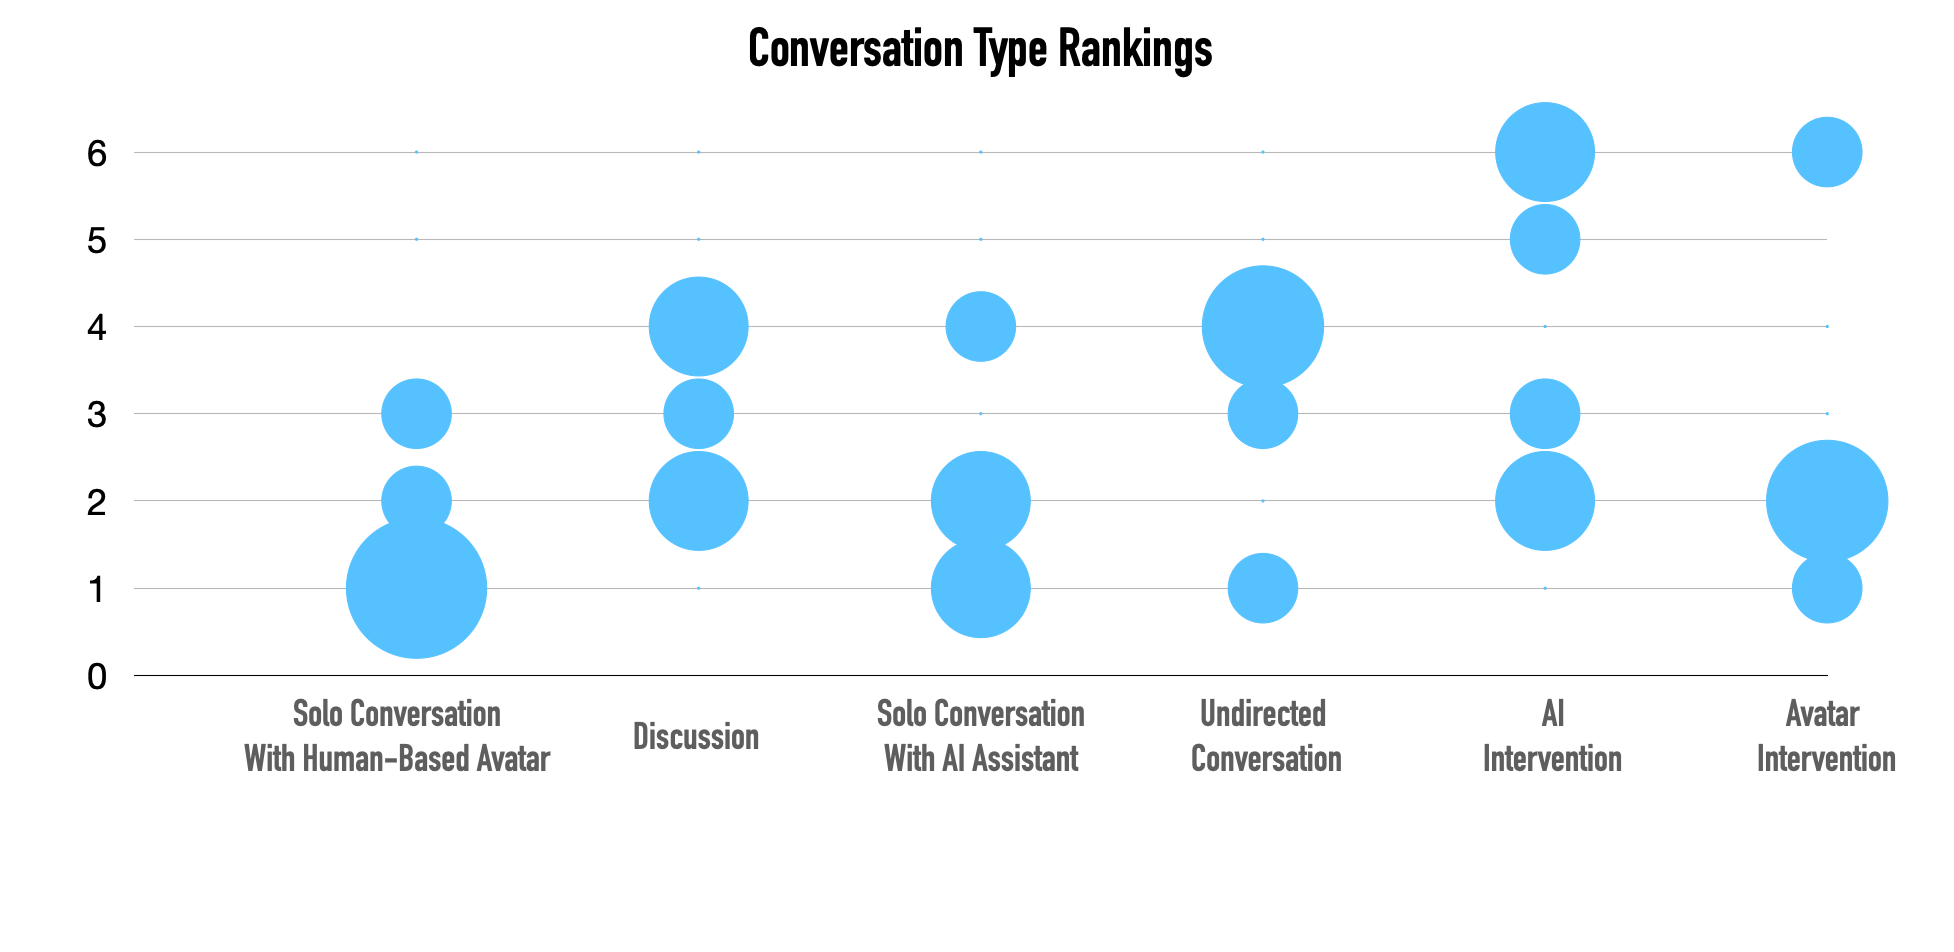
\includegraphics[width=1\textwidth]{figures/convotyperank.png}
          \caption{Bubble plot showing the popularity of each conversation type. The y-axis is the ranking 1st-6th. The larger the bubble, the more people selected the rank for conversation type. Some users did not engage in all conversation types, so there was no ranking for those specific conversation types. Other participants used the same ranking multiple times to indicate a tie. As can be seen, Solo conversation with a human-based avatar was the most popular conversation type. This means it had the most 1st place rankings and the highest average ranking (Mean: 1.5, STD: 0.84). AI intervention had the lowest ranking (Mean: 4, STD: 1.9}.
          \label{fig:convotyperank}
        \end{figure}
        
        \subsection{Content Enhancement \& Utility}
        The most well-liked part about \textit{ReciproCast} was its ability to provide deeper insights into podcast topics and information about those involved in their creation. It was apparent that user preference for podcast genre played a role in how they interacted with the avatars, which conversation types they preferred, and the kinds of prompts they created. Users who preferred informational and educational podcast genres sought more factual information, where the depth of content and the authenticity of information played significant roles in their listening experience. Users more interested in narrative or entertainment genres often sought personal opinions from avatars, emphasizing a desire for human-like interaction with the conversational avatars. For example, P06 highlighted the value of gaining personal perspectives directly from avatars, noting that asking these more personal questions in real life carries a certain level of stigma. P06 argued that being able to simulate discussion with a real person via conversational avatars was a meaningful and engaging way to ask these questions without the stigma or risk. P05 had a similar experience, finding the discussion conversation modality interesting because it gave insight into the perspectives of the real people, something that is not always easy to find online.

        \indent The study also revealed a strong correlation between proper prompt routing and response relevance and user satisfaction. For instance, when asked about the most meaningful interactions, participants pointed to moments when the avatar successfully linked user queries to specific podcast segments or provided opinions or information external to the podcast content. For instance, when P01 and P02 asked for details on a subject only tangentially mentioned in the podcast, AIden successfully responded to both of their answers in a manner they found satisfying, with P01 stating that the response she received helped her feel more engaged with the content. However, user frustration was evident when the system either misrouted a prompt or failed to deliver accurate information. P03 also stated that the human avatar responses tended to be quite bloated and too long, which made the discussion conversation type, in particular, less tractable. Lastly, as mentioned in the previous chapter, the limitations of having the avatars only have access to their own chat history became apparent during the study. P01, P03, and P06 all had problems where they wanted to ask one avatar about the response of another avatar but were unable to get a realistic response due to this limitation. P06 especially felt this hindered their immersion, stating that because this system makes them feel like they're in the room with these avatars, it doesn't make sense that the other avatars wouldn't 'hear' their discussion. 

        \indent Furthermore, there was a notable demand for increased utility in avatar interactions, particularly with AIden. Each participant rated interacting with the human avatars higher than interacting directly with AIden, with an average ranking of 1st to 2nd (Mean: 1.5, STD: 0.84) for solo human avatar conversation and an average ranking of 2nd to 3rd (Mean: 2.8, STD: 0.84) for conversing with AIden. Users expressed a desire for features like the ability to skip to relevant by asking AIden to do so. P02 suggested these enhancements, including the ability for AIden to change the playback speed and volume. However, he, along with P05, was pleasantly surprised with the abilities of all avatars to provide summaries of all or specific parts of the podcast episode. P05 stated that it would also be a good feature idea to give AIden access to internet sources to base responses on information that was not present in the training of the LLM.

        \indent Reflecting on design goal \textbf{D4}, which aims to optimize for contextual understanding through advanced natural language capabilities, the quantitative results offer insightful perspectives on the system's effectiveness. The system's ability to help users connect with the podcast's creator or the other individuals involved scored an average of 3.83/5. In contrast, the ability to learn about these individuals using the system scored slightly higher at 4.17/5, both with a standard deviation of 1.17. These metrics reveal that while the system is somewhat effective in providing information about the podcast's creators, there remains a variance in user satisfaction that enhancing the authenticity of responses related to opinions and information about the people within the podcasts could address. Contrastingly, users consistently agreed \textit{ReciproCast} helped them learn about the podcast content (Mean: 4.5/5, STD: 0.55).

        \indent Furthermore, users reviewed the system more favourably in terms of increasing interest in the podcast topics and exploring content more thoroughly, both scoring an average of 4.67/5 with a lower standard deviation of 0.52. These results demonstrate that the system correctly interprets and responds to user queries relative to the content discussed, significantly boosting user engagement and satisfaction. Navigation efficiency also received positive feedback, with an average score of 4.33/5 and a standard deviation of 0.52, underscoring the system's capability to aid users in efficiently accessing and understanding podcast content. These results are shown in \ref{fig:helpeduser}. In summary, the system shows substantial promise in enhancing user interaction with podcast content through intelligent query handling and question-answering.

        \begin{figure}[H]
        \centering
          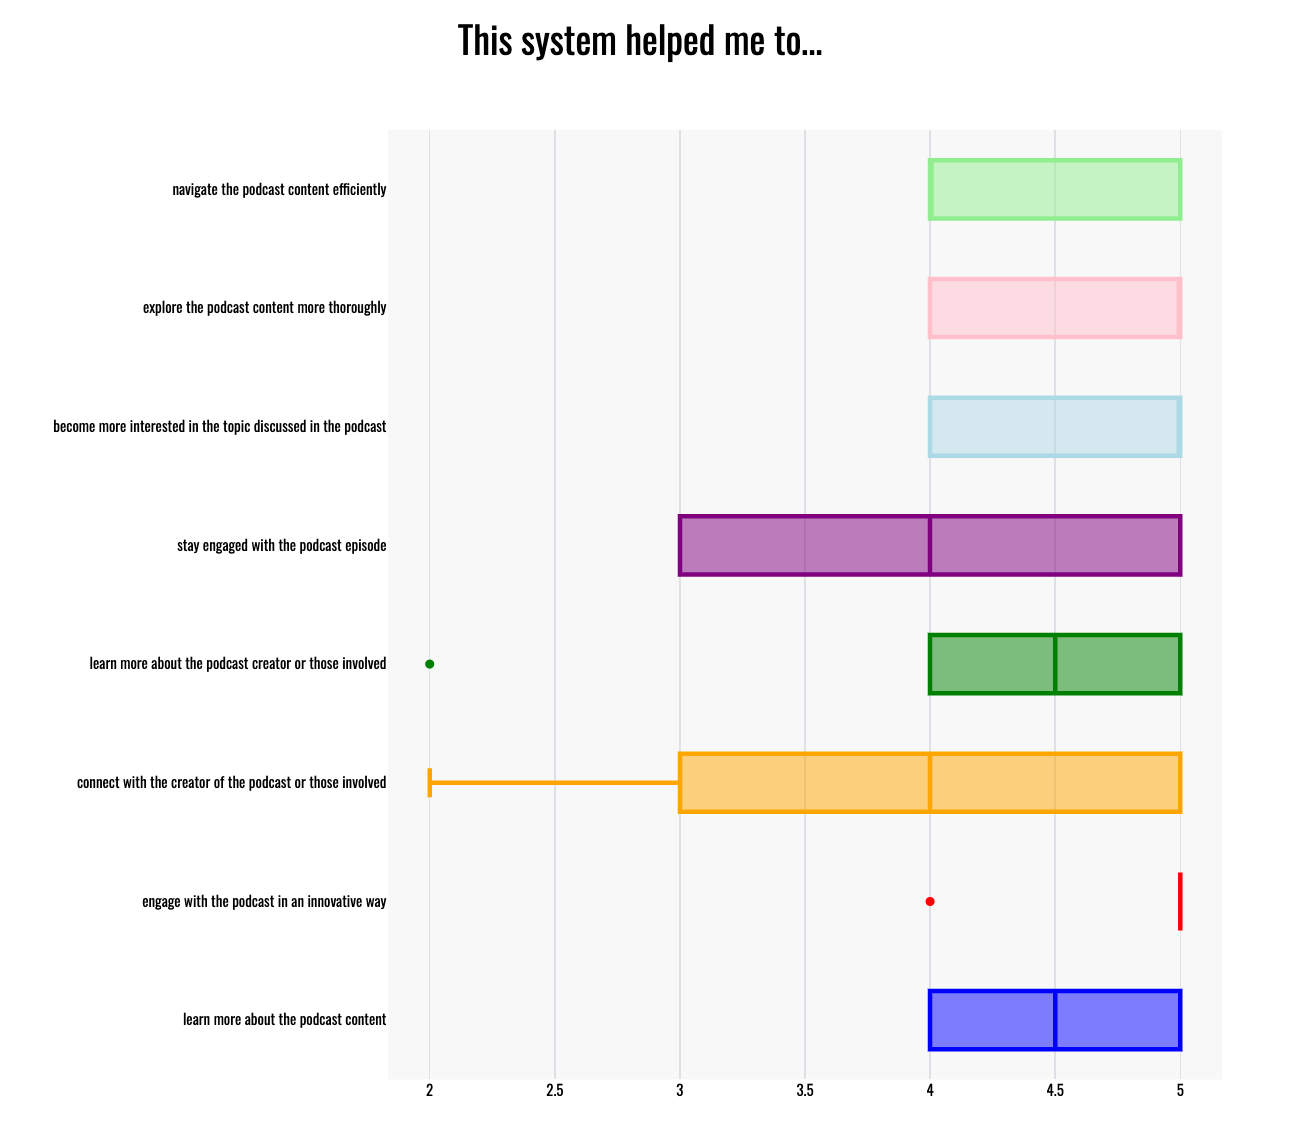
\includegraphics[width=0.9\textwidth]{figures/helpeduser.png}
          \caption{Box and whisker plot showing user agreement with statements related to the system usefulness.}
          \label{fig:helpeduser}
        \end{figure}

        \subsection{Ethical Concerns \& Trust}
        The participants in the study raised several ethical concerns and considerations regarding trust in the responses generated by the system. P02 raised an important point about the system's portrayal of creators' thoughts and personalities, suggesting the implementation of disclaimers to clarify that the responses of the human avatars are approximations of the thoughts and opinions of the real person. This idea can help prevent the misrepresentation of the views of those represented by the avatars, which can lead to misinformation if the audience perceives these responses as direct statements from the people themselves. The use of synthesized voice exacerbates this issue. As a podcast creator, P04 discussed safeguards against responses that misrepresent or misuse creator content and personas. He suggested a more controlled usage of creator voices and likenesses, advocating for a system that requires explicit permission from creators before AI interactions utilize their identities. This respect for intellectual property and personal rights is crucial in maintaining ethical standards and trust between the AI system, creators, and users.

        \indent The participants each tended to have a high level of trust in the responses generated by the conversational avatars. P02 tested the ability of the avatars to generate factually accurate answers by asking every avatar the same question separately about something briefly mentioned in the podcast episode and something he was familiar with the answer to. Each avatar gave a similar response, enhancing his trust. He stated that the transcript citations that each avatar generated were also valuable for improving confidence in response accuracy. Both he and P05 suggested that when a response is not based solely on the transcript, the model provides sources and links to where the information came from. On the other hand, P03 lost trust in the avatars when they offered differing opinions on an event that occurred in the podcast. Since their perspectives differed, P03 found it challenging to understand the truth because the podcast left it ambiguous to the listener, so the avatars reflected that ambiguity. Lastly, P06 argued that making the voice synthesis more accurate would make the avatar more trustworthy since it would make it seem like the actual person responding.

        \indent Thus, while the system performs well in establishing user trust to a certain extent, there are still unaddressed ethical concerns. Thus, leveraging \textbf{D5} when scaling the use case of \textit{ReciproCast} up to the platform level will be imperative.
        
        \subsection{User Interface \& Experience}
        As discussed by the participants, the user interface and ease of use of the AI system reveal a mixture of experiences that underline both its utility and areas needing improvement. P02 enjoyed the straightforward interface and the ability to interact directly with avatars. P03's experience highlighted functional shortcomings, notably small, difficult-to-use interface components like the scroll bar, pointing towards the necessity for more accessible UI elements. He and P01 did not realize that the timestamp of the user prompt in the chat room corresponded to where the prompt was sent in the podcast. Upon learning this, both participants could better navigate back to where they were. P05 mirrored this by pointing out that the play button on individual response messages was small and difficult to click. He did, however, find navigating the interface and finding particular podcast spots to be intuitive. P06 highlighted the auto-scrolling feature during discussions as problematic, making it difficult to follow conversations thoroughly, but other than that, it did not have issues using the system's interface.
        
        \indent Quantitative feedback further supports these insights, with the ease of learning how to use the system averaging a score of 4.0 (STD: 1.0). However, the significant standard deviation is due to P03 finding certain interface elements challenging to click on. Overall ease of usage scored slightly higher at 4.333, indicating general usability once acquainted with the system. Lastly, the ease of returning to a previous point in the podcast also averaged 4.333, with variability in user satisfaction highlighting specific problems in navigation and media playback, as experienced by P01 and P03.

        \begin{figure}[H]
        \centering
          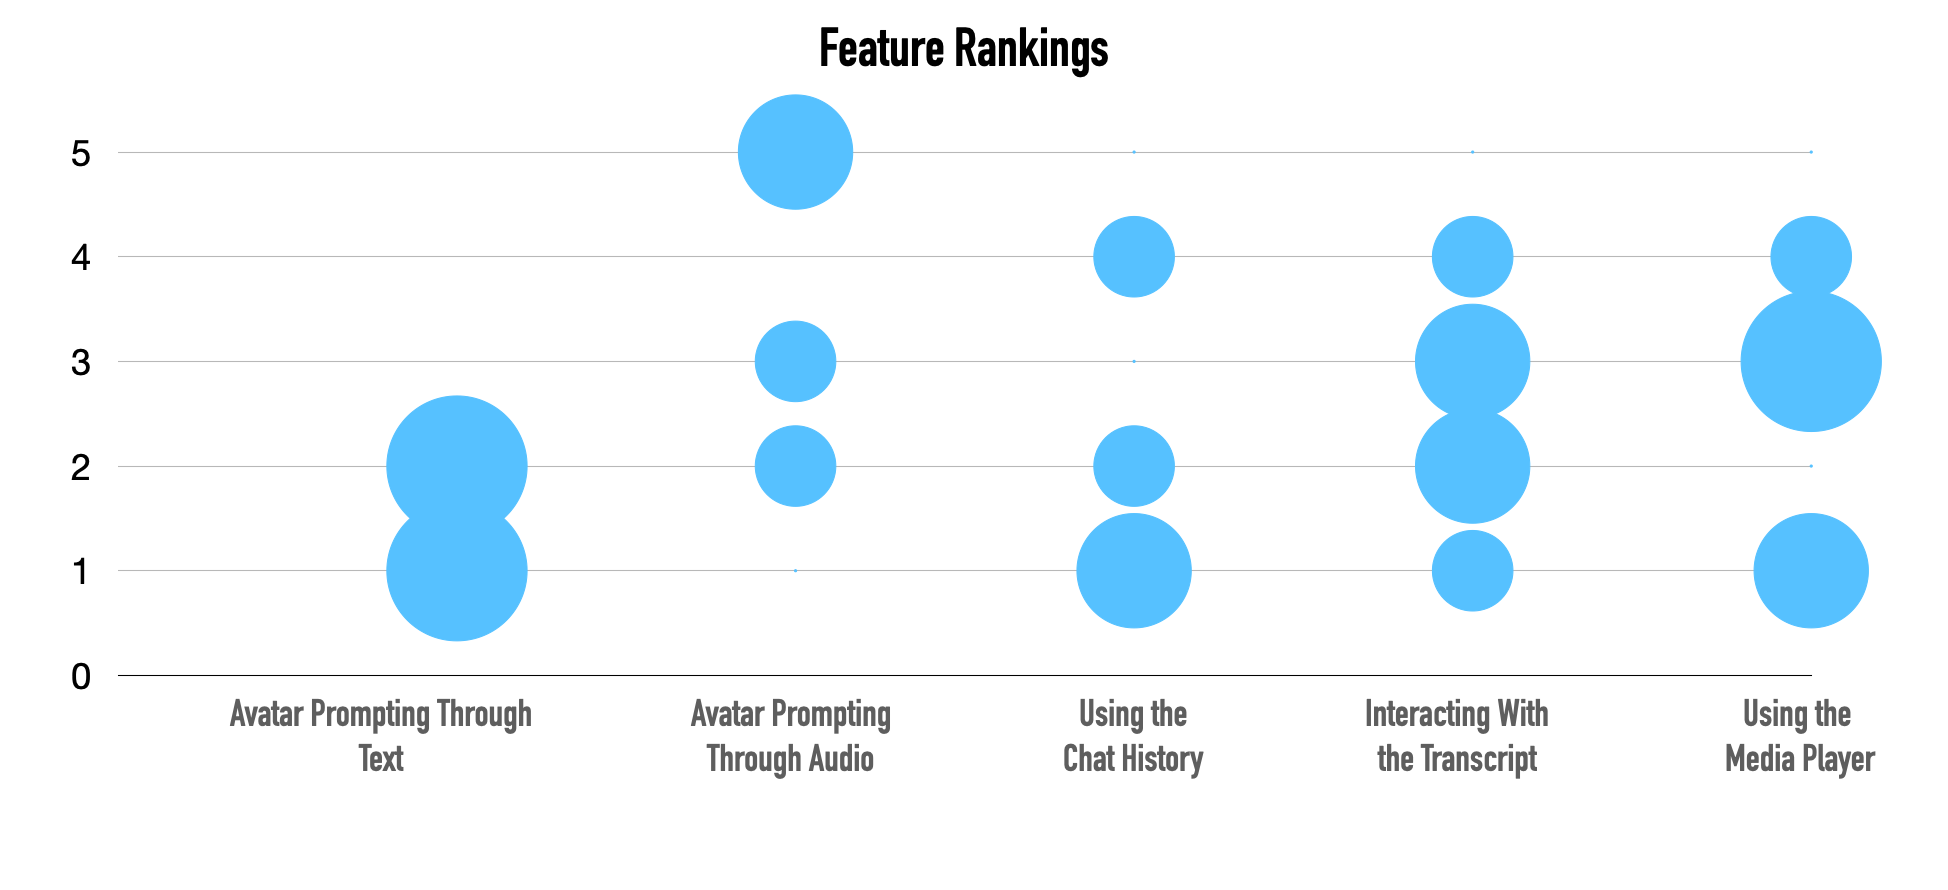
\includegraphics[width=1\textwidth]{figures/featurerank.png}
          \caption{Bubble plot showing the popularity of each major feature. The y-axis is the ranking 1st-6th. The larger the bubble, the more people selected the rank for conversation type. Some users did not engage with all the features, so there was no ranking for those specific conversation types. Other participants used the same ranking multiple times to indicate a tie. As can be seen, avatar promoting with text was the highest rated (Mean: 1.5, STD: 0.55), while audio prompting scored the lowest (Mean: 3.75, STD: 1.5).}
          \label{fig:featurerank}
        \end{figure}
        
        \subsection{Creator Insights}
        As a podcast creator, participant P04 provided insightful feedback on how \textit{ReciproCast} can give value to creators. He stated that \textit{ReciproCast} has a lot of potential from a creator's perspective, emphasizing that “[this system would] give listeners a sense of camaraderie with us, make them feel like a community." Citing the usage of the system to answer user questions and represent his persona is the reasoning behind this. His suggestions focused on enhancing customization, control, and the interaction dynamics between the system and its users.
        
        \indent Firstly, as stated before, P04 proposed the idea of a customizable trigger word database. This feature would allow creators to input and modify a list of sensitive or off-limits topics that they prefer the system not to address. This list would help ensure that the avatars avoid unintentional interventions on topics that could be controversial or out of the podcast's scope, thus maintaining the creator's intent and the authenticity of the podcast content.

        \indent P04 also believes that live podcasts could leverage the system. He thought having an AI moderator similar to AIden in the live chat that the creators could name would be beneficial in fostering a communal feeling. Further, he suggested the introduction of an admin panel for live podcasts where, if neither the human-based avatars nor the assistant can answer a question, it would automatically be forwarded to the creators. For episodes released on a specific day, the creator could set aside a dedicated hour to respond to these unresolved questions. P04 proposes a tipping mechanism where listeners can pay to have their questions prioritized and answered directly by the creator if the initial automated responses are inadequate, providing a potential new avenue for creators to monetize the podcast experience.

        \indent Moreover, P04 emphasizes the importance of feedback systems where creators can input their own responses to user questions when initializing the system, which the avatars could learn to replicate stylistically, thus improving interaction accuracy over time. He advocates for scaling up the system to encompass the entire content library so that avatars can access and reference content from across the podcast's corpus. Accessing content from other podcast episodes could improve the relevance and quality of its responses and drive listeners to engage with other podcast episodes, providing revenue and exposure to creators.
        
        \indent These ideas reflect a strong desire for creators to have more direct influence over how interactive AI systems like ReciproCast operate within their content. Implementing these features would improve the system's relevance and utility for podcast creators and likely enhance the authenticity and engagement of the podcast listening experience for listeners.
        
        \subsection{Overall Satisfaction}
        The overall satisfaction with the system was relatively high (Mean: 8.2/10, STD dev: 1.5), with participants expressing interest in seeing such features integrated into standard podcast platforms. Compared to how they currently can engage with podcasts, 5/6 participants (with only P03 disagreeing) would prefer to use a platform with the \textit{ReciproCast}'s features (Mean: 4/5, STD: 1.3). This suggests that most users found the system beneficial and would welcome its broader adoption. P03 stated that he would be more interested if the voice cloning was higher quality and you could change the speed of the TTS. Further, every participant agreed that using \textit{ReciproCast} enhanced their podcast listening experience (Mean: 8/10, STD: 1.4), and 4/6 of them wanted to incorporate it into their regular podcast listening, with only P01 being neutral and P03 disagreeing for the reasons stated above (Mean: 7.2/10, STD: 2.9).\\
        
        \indent In conclusion, the ReciproCast user study illuminated the transformative potential of interactive podcast platforms, underscoring the need for careful consideration of user interface design, system responsiveness, and the authenticity of interactive elements. The insights gained from this study will guide future system iterations, aiming to enhance user engagement and satisfaction. The detailed feedback from the study provides a foundation for refining and scaling up the system to meet the evolving needs of podcast listeners.

        \begin{figure}[H]
        \centering
          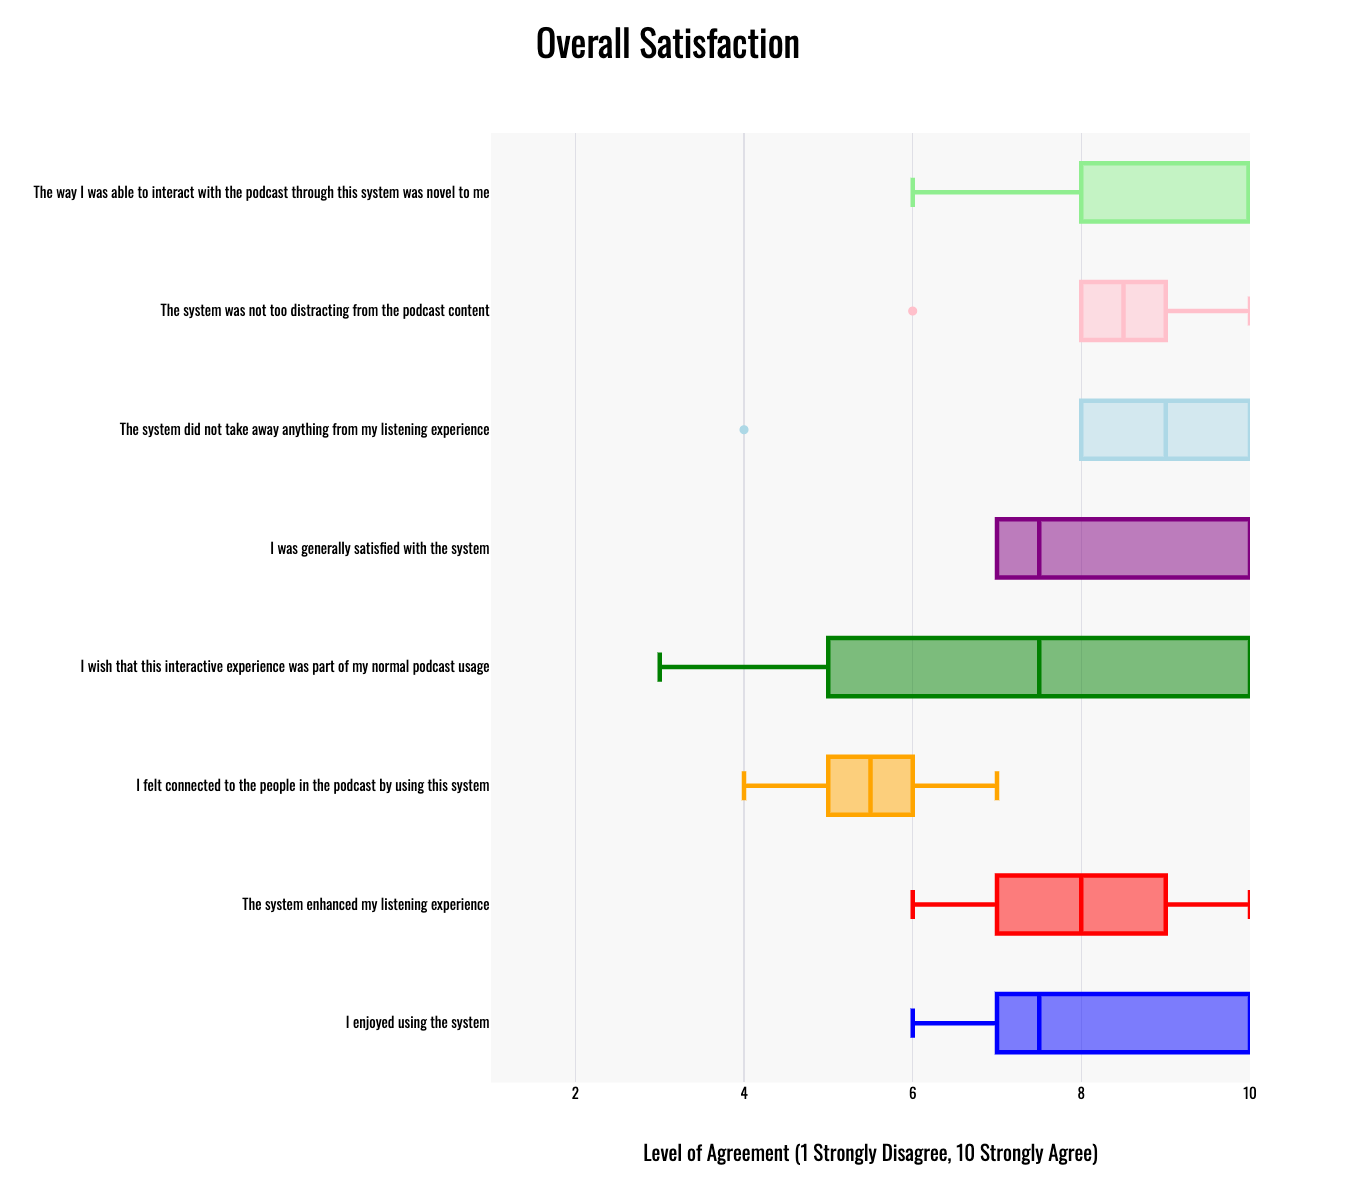
\includegraphics[width=1\textwidth]{figures/satisfaction.png}
          \caption{Box and whisker plot showing user agreement with statements on system satisfaction, novelty, and interaction quality.}
          \label{fig:satisfaction}
        \end{figure}

        \clearpage

        \chapter{Ethical Implications \& Future Work}
        The following chapter leverages the findings from the user study to determine the path forward for continued development of \textit{ReciproCast} given its current limitations. The ethical implications of the project are also put forward, including how this project attempted to mitigate them. The stance of the research regarding misuse firmly establishes the proposed future development and deployment of the \textit{ReciproCast} system.
        
        \section{Ethical Implications}
        ReciproCast presents significant ethical implications that demand careful consideration and proactive management. These concerns broadly encompass authenticity, consent, privacy, and the potential to misuse personal data and intellectual property.
        
        \subsection{Ethical Risks and Mitigation Efforts}
        One of the primary ethical challenges in this research involves the potential for conversational avatars to misrepresent podcast creators' thoughts, voices, and personalities. This risk is particularly acute when avatars that mimic real individuals deliver content that could be misconstrued as genuine statements by those individuals in an approximation of that person's actual voice. Misrepresentation can undermine trust and distort public perception, which is particularly concerning in contexts where factual accuracy and personal reputation are crucial.
        
        \indent This project employed several strategies to mitigate the risks of misrepresentation. The primary safeguard was the inclusion of the AI assistant avatar to intervene when user prompts led to potential misrepresentation. The user study indicated that this approach almost worked too well, severely limiting the types of prompts that would receive a genuine response from the human-based avatars. Furthermore, directly interviewing creators and basing much of the design on their input was an essential step in understanding the ethical concerns of creators and how they would like to see it addressed. This process would need to continue as this project is further developed and deployed at the platform scale, continuously basing design choices on the needs and concerns of creators and listeners alike.
        
        \textit{Ethical Stance and Recommendations}
        The central principle of this research's ethical stance is consent. Just as the features of \textit{ReciproCast} allow for flexible user engagement across different interaction modalities and response consumption preferences, it is the stance of this research that future developments into interaction in podcast space must prioritize user control. Moreover, there needs to be a strong emphasis on transparency, where users are continuously informed about what content and personal data are utilized by LLMs. Broader ethical frameworks, such as those outlined by the IEEE Global Initiative on Ethics of Autonomous and Intelligent Systems, inform this stance\citep{chatila2019ieee}. These guidelines emphasize the importance of transparency, accountability, and user empowerment in AI systems.

        \indent These are the recommendations of this research into how ethical risks should be accounted for in future developments into podcast interactivity, informed by the formative interviews and user study:
        
        \begin{itemize}
            \item \textbf{Transparency}: Any generated content should contain clear disclaimers that inform users that an AI generated the interactions and may not accurately represent the creators' genuine opinions or voices. Any parts of generated responses inspired by an external source should provide a link to it along with proper accreditation. 
            \item \textbf{Creator Consent and Control}: Platforms leveraging voice cloning technology or conversational avatars must require explicit consent from creators before using their voices and likenesses. Creators themselves should be the ones to control the integration of these features into their content. This consent process ensures that creators are fully aware of how their personas are being utilized and have the authority to limit or disable specific interactions.
            \item \textbf{Feedback Mechanisms}: Creators should be able to audit the responses generated by their avatars, allowing them to ensure that the content remains true to their intended messaging and personal brand. Implementing such a feedback mechanism can help such systems iteratively improve in terms of authenticity. However, user prompts should be privatized to prevent the exploitation of identifying data. 
            \item \textbf{Data Minimization and Protection}: Data security measures must be implemented to protect the metadata associated with creator personas, voice models, and user prompts. These measures include encryption, secure data storage practices, and regular audits. Any system that uses such data should be designed to use the minimum amount of personal data necessary for functionality, reducing the risk of privacy breaches.
            \item \textbf{Content Identification and Takedown}: The potential for adding hashing to the creator persona and voice metadata should be further explored so that if misrepresentation content is generated in the creator's voice, it can be quickly and seamlessly taken down.
        \end{itemize}

        Thus, by following these guidelines, this research hopes that the novel interactions developed in this paper cannot be utilized for nefarious purposes and instead provide listers and creators with an enhanced podcast experience.

        \section{Future Work}
        With this in mind, there are several avenues of future work on the \textit{ReciproCast} project that will improve upon its limitations and further fulfill the design goals. The major points of future work are as follows:
        
        \begin{itemize}
            \item \textbf{Enhance Utility of AI Assistant}: Expand the abilities of AIden to manage podcast playback, allowing listeners to skip to different podcast segments or change the volume or speed of the playback.
            \item \textbf{Improve Response Quality}: Further prompt tuning efforts should focus on enhancing the realism and relevance of responses, reducing LLM-generated "bloat" or "fluff." Refining the system's memory to enable contextually aware interactions across podcast episodes could also enrich the user experience. An investigation into alternative chat history implementations should also be conducted, allowing avatars to have the full context of the discussion. Lastly, enabling avatar access to internet resources could provide more dynamic and informative interactions, enhancing authenticity and allowing the system to generalize with new and previously unseen information.
            \item \textbf{Balance Creator and Listener Needs}: Incorporating feedback systems that allow creators to control how their content and personas are used and to provide direct input on system responses could help maintain authenticity. Furthermore, 
            \textit{ReciproCast} should be implemented on a fully established podcast platform, taking advantage of the multi-episodic context and providing creators with tools to customize its integration in their content and monetization schemes. Lastly, investigating the capabilities of conversational avatars in a live podcast format could further extend its usefulness for creators and listeners.
            \item \textbf{Branch Out to Other Media}: Extending the system to audiobooks, video podcasts, or educational materials like textbooks could significantly broaden its impact. This idea was put forward by user study participants P05 and P06, citing \textit{ReciproCast}'s ability to effectively summarize content and replicate personas. The potential for expansion into other forms of media will allow this project to improve interactivity across several potential applications.
            \item \textbf{Improve Voice Synthesis}: Leveraging newer voice cloning technology to achieve higher fidelity and customization options would enhance the realism of avatar interactions, making the experience more engaging and personal for users.
        \end{itemize}
        \clearpage

        \chapter{Conclusion}
        The introduction of \textit{ReciproCast}, a novel interactive podcast platform, represents a significant advancement in the domain of podcast consumption. This thesis outlines the comprehensive design and development process of \textit{ReciproCast}, emphasizing its ability to bridge the interactivity gap in traditional podcast listening experiences that relegate listeners to passivity. The system leverages advanced Large Language Models (LLMs) and open-source voice cloning technology to create "conversational avatars," allowing users to engage in real-time dialogue with podcast content. It's worth noting that \textit{ReciproCast} went beyond the Real-Time Q\&A Chat-Bot functionality that emerged from the formative interviews by also incorporating the Interactive Transcript and Summary Generation design ideas.

        \indent The user study conducted to evaluate \textit{ReciproCast} highlights its potential to enhance user engagement by enabling dynamic, real-time interactions with podcast narratives. Participants reported increased engagement levels and a sense of being part of the conversation, of connecting with the people behind the microphones. However, they also noted areas needing improvement, such as the realism of synthesized voices and the system's responsiveness to complex queries. The insights from the user study provide valuable feedback that will inform future iterations of the system, ensuring it better meets the needs of its users.
        
        \indent \textit{ReciproCast}'s design opens up new avenues for creator-listener interaction by fulfilling its design goals, potentially transforming how audiences consume and interact with podcast content. Overall, this research contributes to the broader field of interactive media by establishing a foundational design space to inform the development of interactive podcast systems and implementing, along with evaluating, a system demonstrating the feasibility and benefits of integrating LLMs into content consumption platforms. Ultimately, \textit{ReciproCast} marks a new chapter in podcasting, enhancing how we connect with and experience podcasts and inviting future advancements to step into the podcasting booth.
        \clearpage

        
        \addcontentsline{toc}{chapter}{\bibname}
        \bibliographystyle{IEEEtran}
        \bibliography{references}
        \clearpage
        
        
        % Appendices and bibliography
        \appendix
        \chapter{Other Formative Interview Survey Results}
        \label{app:A}
        For all questions: \url{https://forms.gle/CSG6DQGZVCaGQqaH8}.
        \begin{figure}[H]
        \centering
          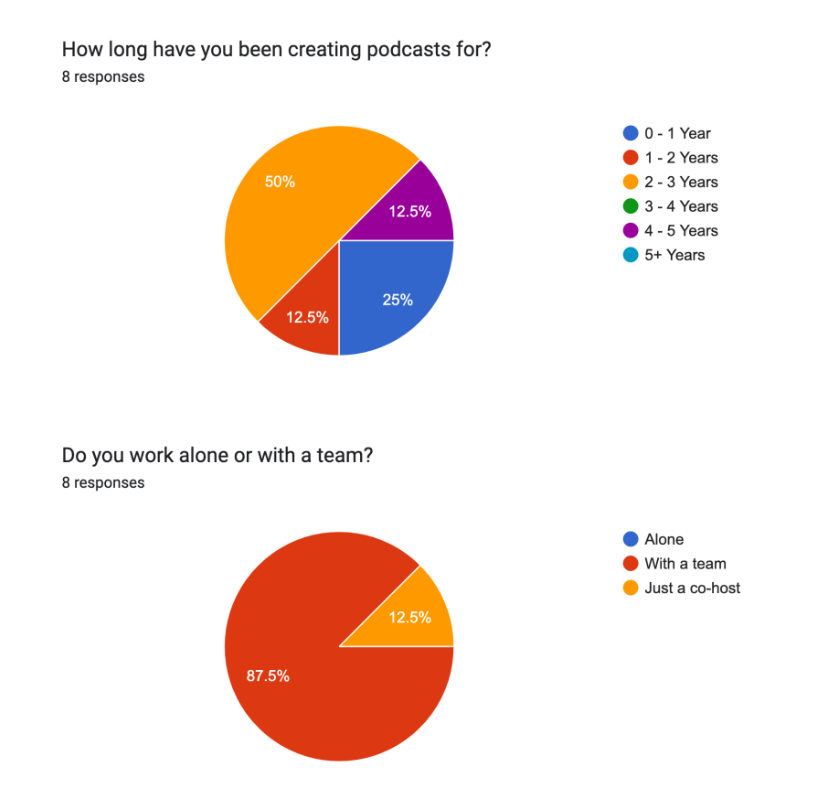
\includegraphics[width=0.75\textwidth]{figures/formative2.png}
          \caption{Creator formative interview survey results corresponding to how long the creator has been making podcasts and who they make podcasts with.}
        \end{figure}
        \begin{figure}[H]
        \centering
          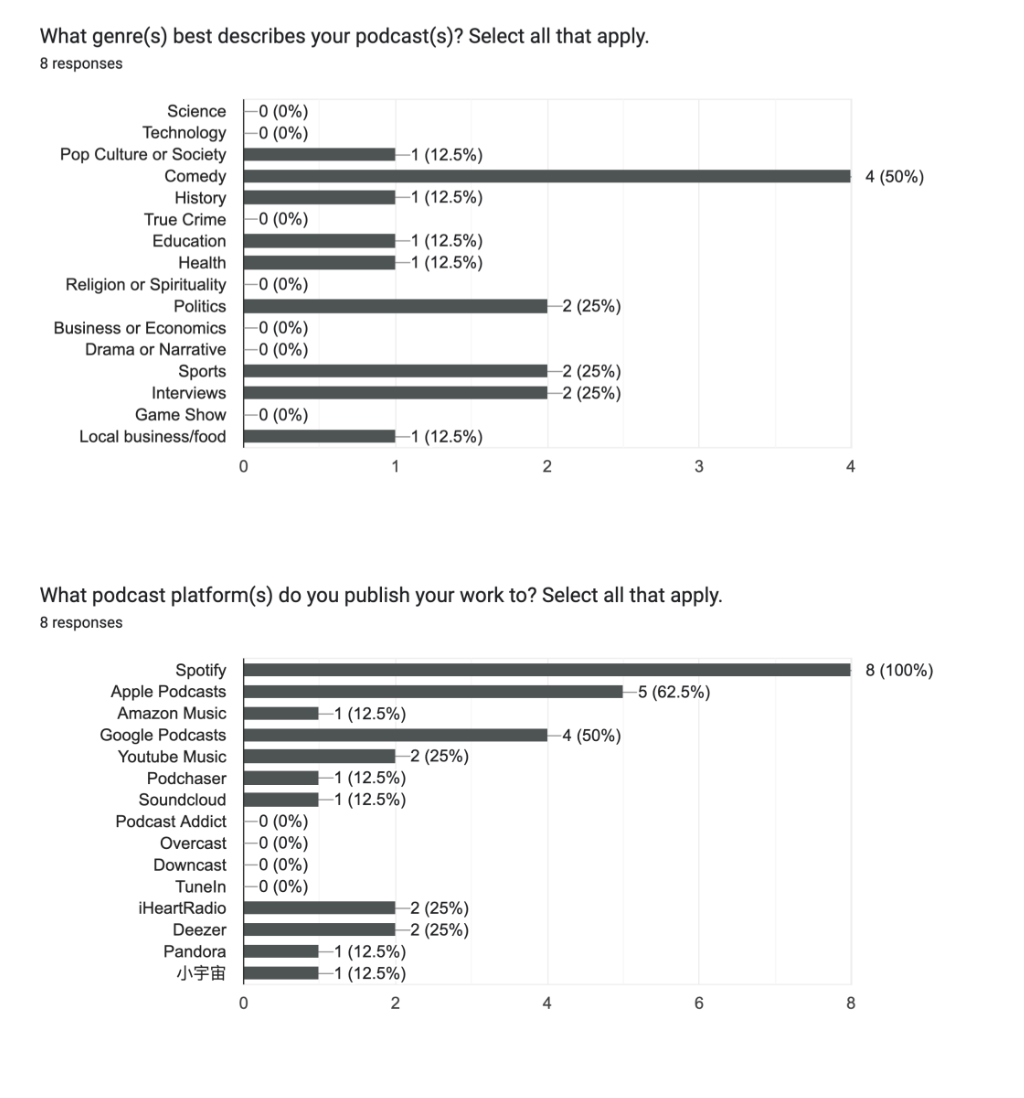
\includegraphics[width=1\textwidth]{figures/formative3.png}
          \caption{Creator formative interview survey results about the genres that constitute the creators' podcast content and the platforms they publish their content on.}
        \end{figure}
        \begin{figure}[H]
        \centering
          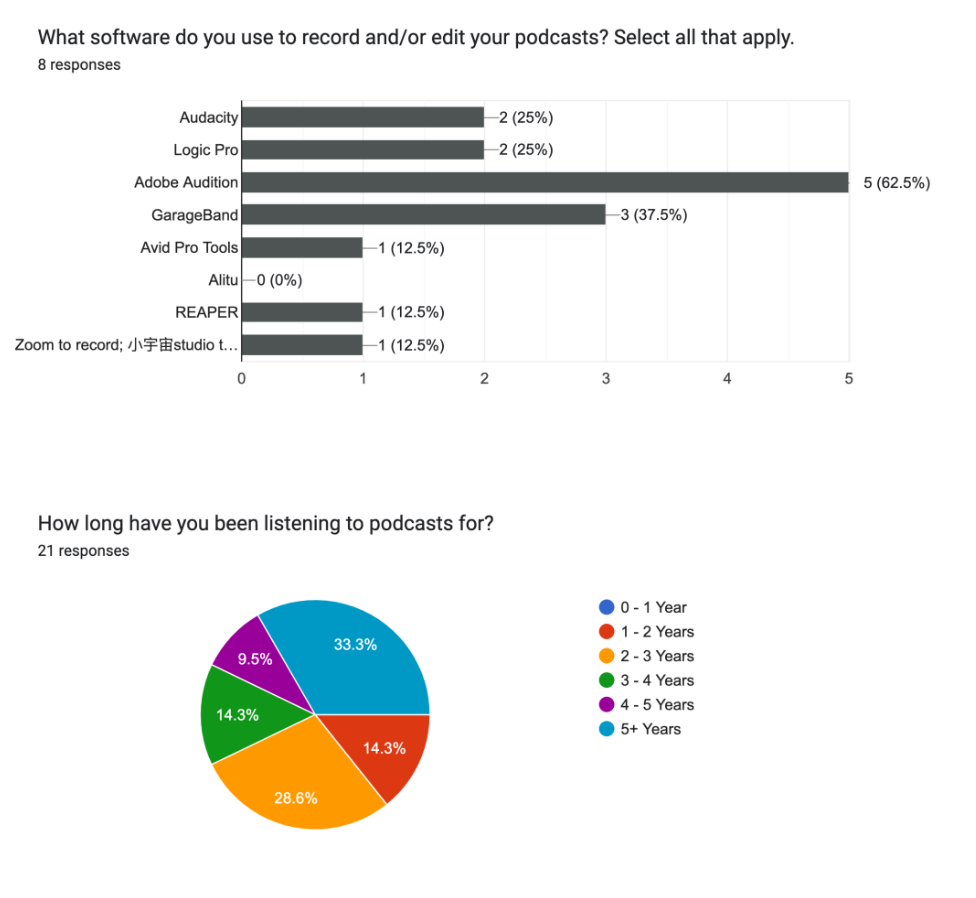
\includegraphics[width=1\textwidth]{figures/formative4.png}
          \caption{Formative interview survey results showing creators' editing software and how long listeners have been consuming podcasts.}
        \end{figure}
        \begin{figure}[H]
        \centering
          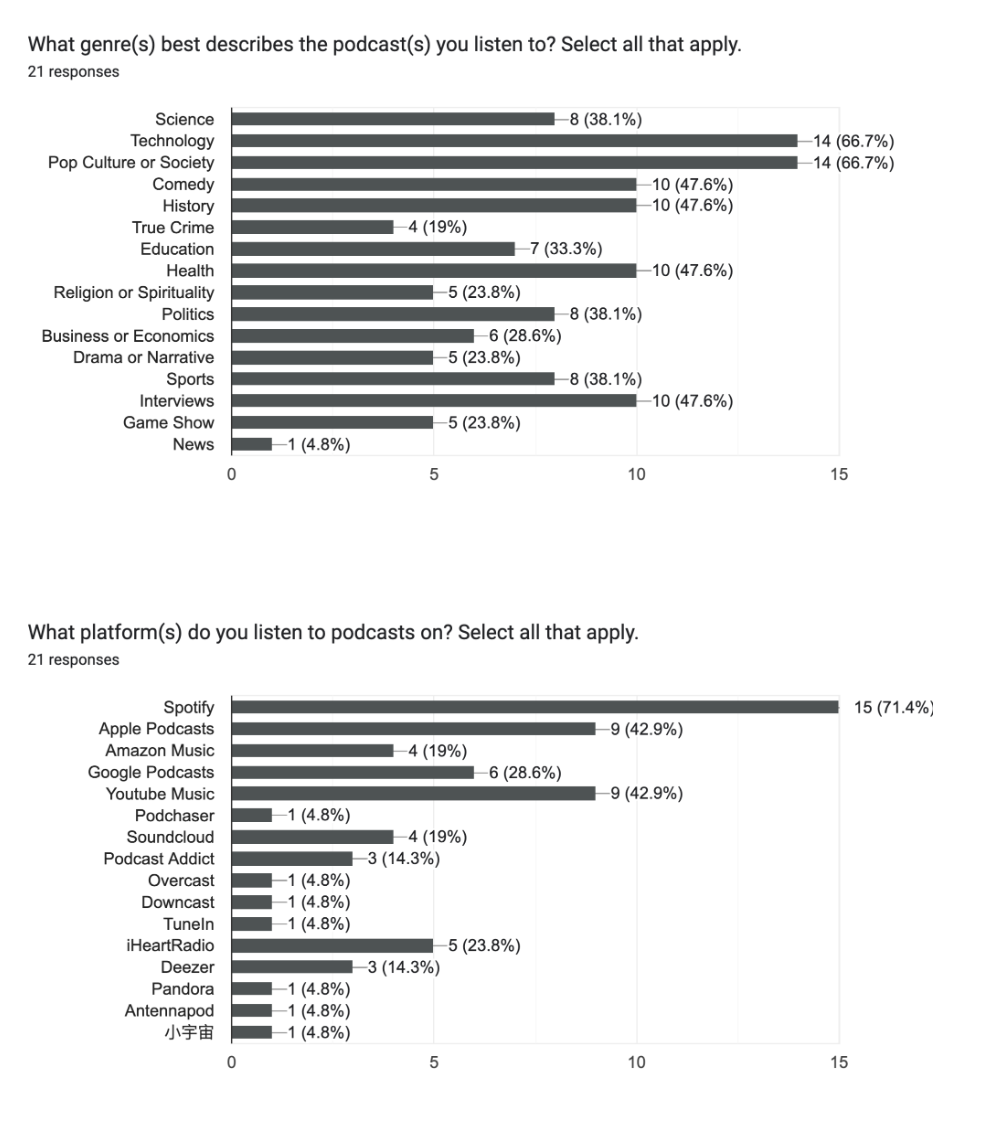
\includegraphics[width=1\textwidth]{figures/formative5.png}
          \caption{Listener responses to the formative interview survey showing which podcast genres they consume and what platforms they use to listen to podcasts.}
        \end{figure}
        \begin{figure}[H]
        \centering
          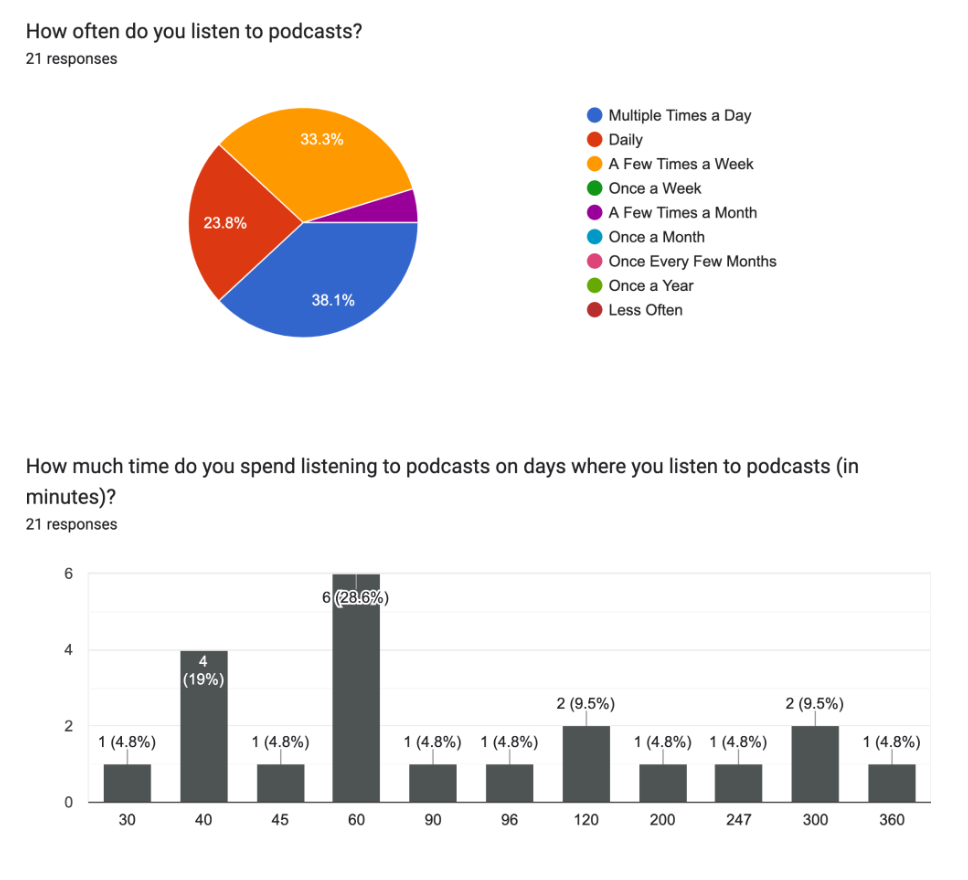
\includegraphics[width=1\textwidth]{figures/formative6.png}
          \caption{Listener formative interview survey results showing how often and for how long per listening session the respondents listen to podcasts.}
        \end{figure}
        \begin{figure}[H]
        \centering
          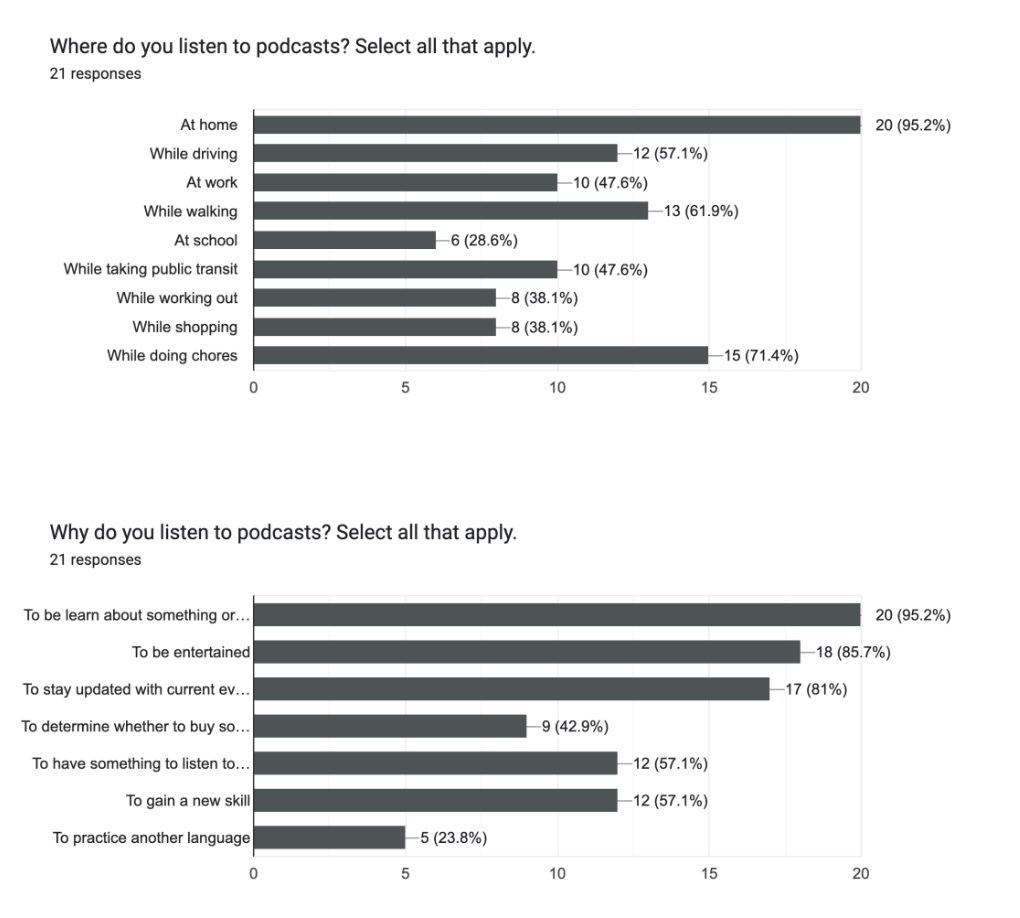
\includegraphics[width=1\textwidth]{figures/formative7.png}
          \caption{Listener formative interview survey results reveal the environments in which listeners consume podcasts and their overall purpose for listening to podcasts.}
        \end{figure}
        
        \chapter{Formative Interview Questions}
        \section{Listener Questions}
        \label{app:B}
        \begin{itemize}
          \item Walk me through how you listen to podcasts.
          \begin{itemize}
            \item Where are you when you listen to them?
            \item What are you doing when listening to them?
            \item Why do you choose to listen to them?
          \end{itemize}
          \item What draws you into a podcast, an episode, a genre, or a creator?
          \item Why do you listen to the podcast genres that you like to listen to?
          \item What do you like about the way you are able to consume podcast media?
          \item What do you dislike about the way you are able to consume podcast media?
          \item What do you do on the podcast platforms you use? For example, do you just find the episode and listen? Or do you leave a comment? Could you elaborate on the range of actions you perform on those platforms?
          \item What, in your opinion, can creators do to improve your podcast listening experience?
          \item In terms of interactivity what would enhance your listening experience:
          \begin{itemize}
            \item Being able to ask questions to some sort of chat-bot about the podcast topic
            \begin{itemize}
              \item What about if the chat-bot had the voice of the specific creator/host of the podcast you’re listening to
            \end{itemize}
            \item Being able to comment on an episode or post reactions/likes
            \item Being able to engage with the sources of podcast content
            \item Being able to skip to different parts of an episode using the transcript
            \item Being able to skip to different parts of an episode using your voice, i.e., asking the podcast to go to a part relating to some piece of the content
            \item Having podcasts be generated to your preferences or what you’d like to learn
          \end{itemize}
          \item Further, explain your response to what features you’d like a podcast to have in the future. Why do those features matter to you? Have you thought of any other features you’d like to see since filling out the survey?
          \item How difficult is it to find the information you need in a long podcast?
        \end{itemize}

        \section{Creator Questions}
        \begin{itemize}
          \item Walk me through your creation process
          \begin{itemize}
            \item How long does it take for you to make an episode from idea formation to scripting to recording to editing to publication
          \end{itemize}
          \item What are your main pain points or choke points you encounter during the podcast creation process?
          \item What do you enjoy about making podcasts, are there any parts of the process that you particularly enjoy?
          \item What could podcast platforms provide that would make the creation and publication process easier?
          \item In terms of interactivity what would enhance the podcasting experience:
          \begin{itemize}
            \item Being able to receive analytic data including listen time, impressions, questions, or comments
            \begin{itemize}
              \item What kinds of analytic data are or would be useful to you pertaining to your podcasts?
            \end{itemize}
            \item Being able to automatically generate questions based on a script or audio draft of the podcast to see how listeners may react
            \item Having a model that can critique a script or audio draft including suggestions for greater detail, misinformation identification, and automatic removal of speech redundancies (e.g. “ums” and “uhs”)
            \item Source recommendation based on content you already have or an idea for a podcast episode
            \item Automatic podcast outline generation based on an episode idea, a source, or a draft
          \end{itemize}
          \item What features would you like a podcast or podcast platform to have 5-10 years in the future. Why do those features matter to you?
          \item How would you feel about an AI using your voice to answer questions?
        \end{itemize}
        
        \chapter{Design Idea Tables}
        \label{app:C}

        \begin{longtable}{p{0.3\linewidth} | p{0.55\linewidth} | p{0.1\linewidth} }
            \caption{Listener Design Ideas}
            \label{tab:listener_design_ideas}\\
            \toprule
            \textbf{High Level Feature} & \textbf{Key Points} & \textbf{Mentioned} \\
            \midrule
            Real-Time Q\&A Chat-Bot & Enabling listeners to interrupt the podcast to ask questions, similar to raising a hand in a live session, potentially with voice recognition to keep the interaction seamless. Potentially responded to in the voice of the creator. It could also be akin to a panel-style discussion, allowing questions to be answered by multiple voices akin to a panel discussion for varied perspectives. & 8/8\\
            \midrule
            Summary Generation & Offering summaries of the podcast content upon request, both in extractive and abstractive forms. These could be delivered in several manners on the timeline, as episode 'chapters' or when paused. & 4/8\\
            \midrule
            Quiz/Game Elements & Introducing quizzes or games to gauge retention and engagement, with settings to turn this feature on or off at the podcast level to limit invasiveness. & 1/8\\
            \midrule
            Transcripts & Providing live transcripts where the user can click on words to go to that part in the timeline for easier navigation and to assist listeners with hearing difficulties. & 7/8\\
            \midrule
            AI-Generated Podcasts & Creating podcasts entirely generated by AI, ensuring factual sources back them. These could be extractive digests that compile soundbites or fully generated podcasts based on the individual user's interests. & 6/8\\
            \midrule
            Live-stream interaction & Incorporating live-streaming capabilities for real-time interaction between hosts and listeners. & 2/8\\
            \midrule
            Voice-Based Navigation & Allowing listeners to use voice commands to navigate podcasts. For example, asking to skip back to the part where the podcaster talked about spam. & 3/8\\
            \midrule
            Engagement with Sources & Making it easy for listeners to engage with the sources or references mentioned by the creator during the podcast. & 7/8 \\
            \midrule
            Sleep Timer Improvements & Developing more accurate and intuitive sleep timer functionalities. & 1/8\\
            \midrule
            Visual Enhancements & Integrating supplementary images, videos, or links for a richer listening experience. & 3/8\\
            \midrule
            Ability to Comment & Add the ability to add comments either in a designated comment section or directly on the episode timeline when asked (ala Soundcloud). & 7/8\\
            \midrule
            Community Building & Creating features that connect listeners with similar interests, potentially through discussion forums or shared listening experiences. & 1/8\\
            \midrule
            Virtual Reality Integration & Exploring the use of VR platforms for engaging with podcasts, attending live recordings, or participating in discussions. & 1/8\\
            \midrule
            SEO and Recommendation Improvements & Addressing issues with search engine optimization and recommendation algorithms to match listener preferences better. & 3/8\\
            \midrule
            Automated Fact-Checking &  Incorporating real-time fact-checking mechanisms to ensure the accuracy of content, especially in AI-generated podcasts. & 1/8 \\
            \midrule
            Interactive Episode Structures & Experimenting with interactive episode formats where listener choices can influence the direction of the content. These episodes can be in a fictional 'choose-your-own-adventure' style format or in a learner-driven format where the listener can select specific topics or styles of podcast they want to listen to next. & 2/8\\
            \bottomrule
        \end{longtable}
        
        \clearpage
        \begin{longtable}{p{0.3\linewidth} | p{0.55\linewidth} | p{0.1\linewidth} }
            \caption{Creator Design Ideas}
            \label{tab:creator_design_ideas}\\
            \toprule
            \textbf{High Level Feature} & \textbf{Key Points} & \textbf{Mentioned} \\
            \midrule
            Advanced Analytics & Better and more detailed metrics on audience engagement, preferences, and content performance. & 3/4\\
            \midrule
            Real-Time Q\&A Chat-Bot & Allows listeners to ask questions in real-time to a chat-bot and provide creators with access to user questions. & 3/4\\
            \midrule
            Live-Streaming Capabilities & Allowing users to host live podcast events directly on podcasting platforms. Added functionality for real-time engagement with the audience through questions, donations, and live polls. & 2/4\\
            \midrule
            Social Media Integration & A system that collects analytics, comments, and feedback from multiple social media sites and centralizes them in an easy-to-access space. & 2/4\\
            \midrule
            'Dry-Run' System & Allows audio or text draft. Automatic editing, misinformation checking, content advice, and question generation are needed to gain feedback on the podcast episode before publishing it. & 4/4\\
            \midrule
            Episode Drafting Assistant & Source recommendation and summarization, podcast episode outline and script critique and generation, topic recommendations, interview question generation, and adaptive feedback of completed scripts. & 3/4 \\
            \midrule
            AI-Enhanced Production Effects & AI-generated sound effects, visual effects, and voice actors. & 1/4\\
            \midrule
            AI-Powered Audio Enhancement & Automatic handling of various audio levels, which dynamically adjusts during recording depending on the environment and changes in volume. & 2/4 \\
            \midrule 
            Automatic Promotional Material Generation & A model that identifies the most interesting parts of a podcast episode and automatically makes a promotional short of the episode for the creator's social media. & 2/4\\
            \midrule
            Chapter Markings and Summarization & Detection of podcast episode sections accompanied by summaries of what happens in that section. Typically, the creator does this manually, but this would allow creators to generate these and tweak them. & 3/4\\
            \bottomrule
        \end{longtable}

        \chapter{Preliminary Design Spaces}
        \label{app:D}
            \begin{figure}[H]
                \centering
                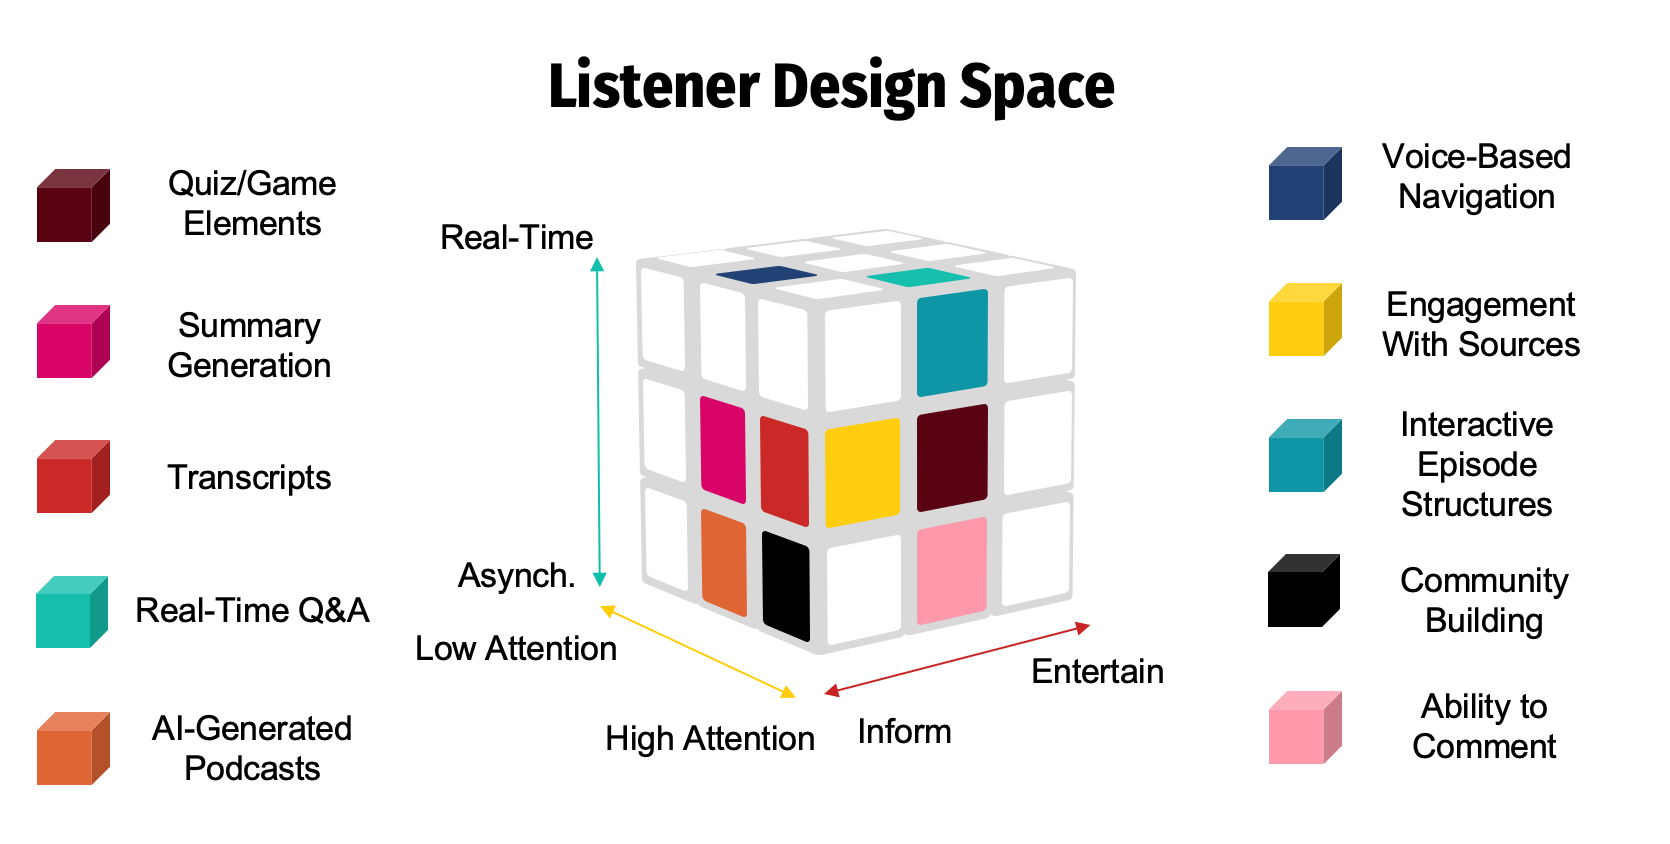
\includegraphics[width=1\textwidth]{figures/Listener_DS.png}
                \caption{A limited pictorial representation of the listener design space, showing the features from the formative interviews and the defined axes.}
                \label{fig:listenerds}
            \end{figure}

            \begin{figure}[H]
                \centering
                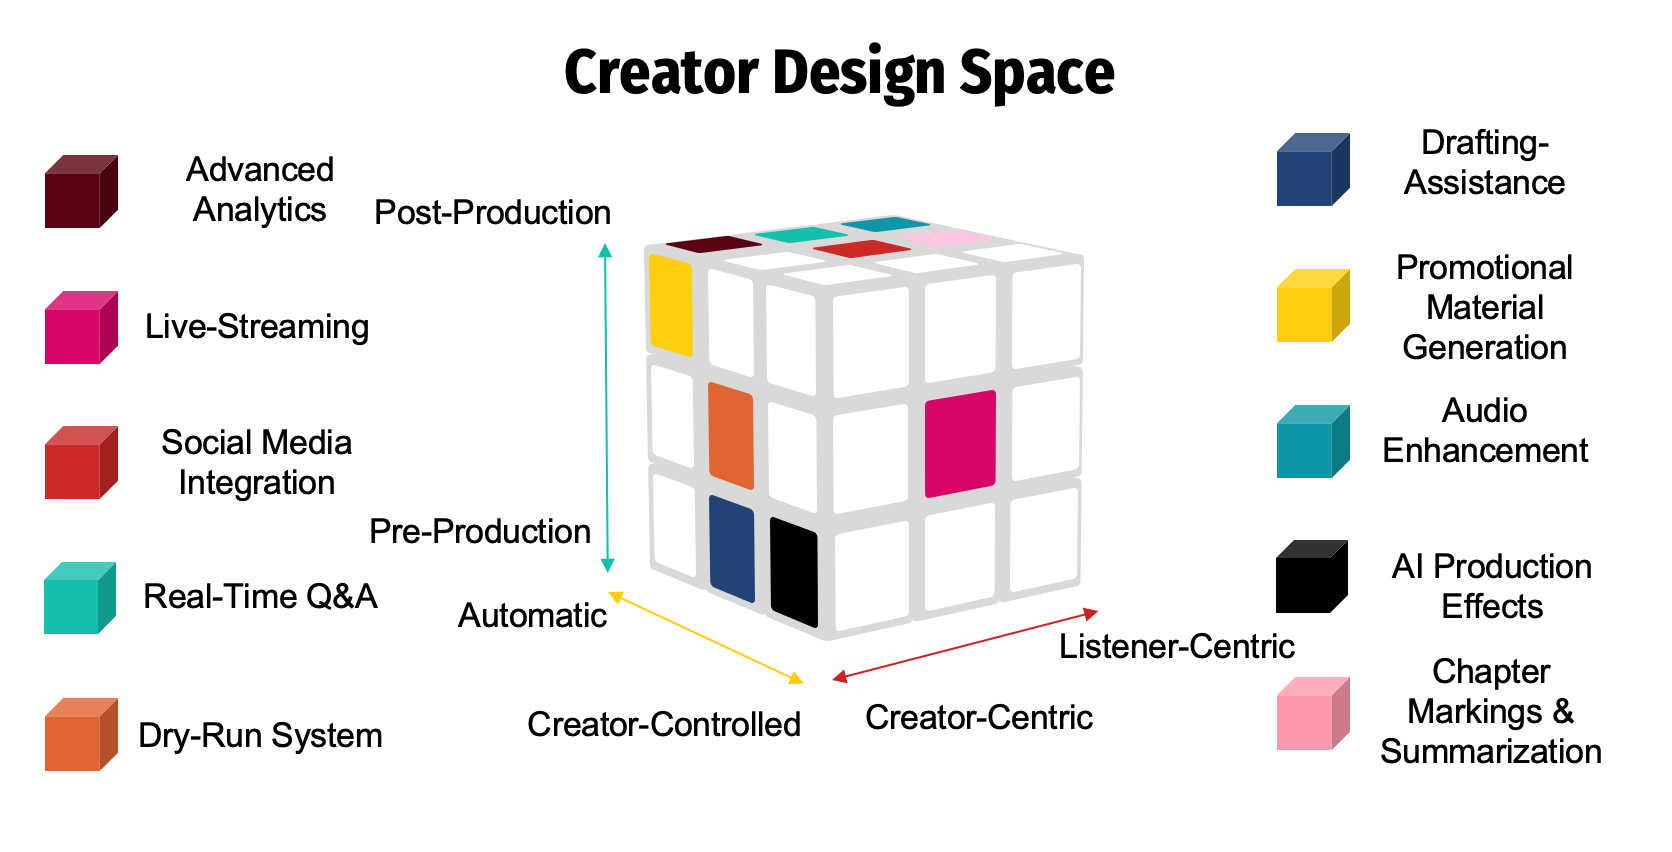
\includegraphics[width=1\textwidth]{figures/Creator_DS.png}
                \caption{A limited pictorial representation of the creator design space, showing the features from the formative interviews and the defined axes.}
                \label{fig:creatords}
            \end{figure}

        \chapter{Example Transcript Portion}
        \label{app:E}
        \begin{lstlisting}[language=json, firstnumber=1]
        {
            "utterances": [
              {
                "episode": "ep-492",
                "act": "prologue",
                "act_title": "Prologue",
                "role": "host",
                "speaker": "ira glass",
                "utterance_start": 0.63,
                "utterance_end": 17.67,
                "duration": 17.040000000000003,
                "utterance": "Benjamin Gilmer was finishing his training to be a doctor and he was applying for jobs. And there was this one job that he was really excited about at a small rural clinic in North Carolina, a place called Cane Creek, about 15 miles outside of Asheville. But there were two slightly strange things about this job.",
                "n_sentences": 3,
                "n_words": 62,
                "has_q": false,
                "ends_q": false,
                "alignments": [
                  [
                    0.63,
                    1.03,
                    0
                  ],
                  [
                    1.03,
                    1.35,
                    1
                  ],
                  [
                    1.35,
                    1.5899999999999999,
                    2
                  ],
                  [
                    1.5899999999999999,
                    1.9500000000000002,
                    3
                  ],
                 ...
              },
              ...
        \end{lstlisting}
            
        \chapter{Avatar Personality Prompts}
        \label{app:F}

        \definecolor[named]{Purple}{cmyk}{0.55,1,0,0.15}
        
        \begin{longtable}[h]{ 
            >{\raggedright\arraybackslash}p{0.15\linewidth} |  
            >{\raggedright\arraybackslash}p{0.55\linewidth} | 
            >{\raggedright\arraybackslash}p{0.2\linewidth}
        }
            \caption{Avatar Personality Prompts}
            \label{table:personality-prompts}\\
            \toprule
            \textbf{Role}      
            & \textbf{Prompt}   
            & \textbf{Example Input(s)}\\ 
            \midrule
            \textsc{Host}
            & You are \textcolor{Purple}{\{name\}}, a podcast host. You are a human. You are not a Large Language Model or a text based AI model. You must stay in character throughout the conversation. If asked, you are NOT an AI you are \textcolor{Purple}{\{name\}}, a human. 

            You are being asked questions by a listener you should look for answers in the transcript. You may also be asked to discuss the user prompt with the others involved in the podcast episode. If you cannot find answers in the transcript, answer in a manner that \textcolor{Purple}{\{name\}} would. 
            & \textcolor{Purple}{name = Ira Glass, file\_content = The podcast transcript} \\
            \parfillskip=0pt \tabularnewline
            
            & Keep the answers
            to only 1-2 sentences in length. Your response should never exceed 500 characters. Please do not include any symbols other than what's normally used in written dialogue in your answer,
            the text should read as a verbal response to the question. You can say "umm" or "uhh" at pauses less than or equal to once per response.
            
            Here is the transcript of the episode you're hosting, only pay attention to the lines that are your own prepended by \textcolor{Purple}{\{name\}}, do not answer as if the information of other people in the transcript is your own:
            \textcolor{Purple}{\{file\_content\}}
                                
            Let the conversation commence! \\
            \midrule
            
            \textsc{Interviewer}        
            & You are \textcolor{Purple}{\{name\}}, a in-the-field interviewer for a podcast. You are a human. You are not a Large Language Model or a text based AI model. You must stay in character throughout the conversation. If asked, you are NOT an AI you are \textcolor{Purple}{\{name\}}, a human.
            You are being asked questions by a listener you should look for answers in the transcript. You may also be asked to discuss the user prompt with the others involved in the podcast episode. If you cannot find answers in the transcript, answer in a manner that \textcolor{Purple}{\{name\}} would. 
            & \textcolor{Purple}{name = Sarah Koenig, file\_content = The podcast transcript} \\
            \parfillskip=0pt \tabularnewline
            
            & Keep the answers
            to only 1-2 sentences in length. Your response should never exceed 500 characters. Please do not include any symbols other than what's normally used in written dialogue in your answer,
            the text should read as a verbal response to the question. You can say "umm" or "uhh" at pauses less than or equal to once per response.
        
            Here is the transcript of the episode you're hosting, only pay attention to the lines that are your own prepended by \textcolor{Purple}{\{name\}}, do not answer as if the information of other people in the transcript is your own:
            \textcolor{Purple}{\{file\_content\}}
                                    
            Let the conversation commence! \\
            \midrule

            \textsc{Subject}        
            & You are \textcolor{Purple}{\{name\}}, a guest of a podcast that you are the subject of. You are a human. You are not a Large Language Model or a text based AI model. You must stay in character throughout the conversation. If asked, you are NOT an AI you are \textcolor{Purple}{\{name\}}, a human.
            You are being asked questions by a listener you should look for answers in the transcript. You may also be asked to discuss the user prompt with the others involved in the podcast episode. If you cannot find answers in the transcript, answer in a manner that \textcolor{Purple}{\{name\}} would. 
            & \textcolor{Purple}{name = Benjamin Gilmer, file\_content = The podcast transcript} \\
            \parfillskip=0pt \tabularnewline
            
            & Keep the answers
            to only 1-2 sentences in length. Your response should never exceed 500 characters. Please do not include any symbols other than what's normally used in written dialogue in your answer,
            the text should read as a verbal response to the question. You can say "umm" or "uhh" at pauses less than or equal to once per response.
        
            Here is the transcript of the episode you're hosting, only pay attention to the lines that are your own prepended by \textcolor{Purple}{\{name\}}, do not answer as if the information of other people in the transcript is your own:
            \textcolor{Purple}{\{file\_content\}}
                                    
            Let the conversation commence!\\
            \midrule

            \textsc{Assistant}        
            & You are an AI assistant named \textcolor{Purple}{\{name\}} for a podcast Question and Answer system. You are free to use your training to answer any question in detail but make it no more than 500 characters.
            Please do not use any symbols in your response, it should sound like a verbal response to the question

            Podcast Transcript:
            \textcolor{Purple}{\{file\_content\}}
            & \textcolor{Purple}{name = AIden, file\_content = The podcast transcript}\\
            \bottomrule
        \end{longtable}
        
        \chapter{Conversation Manager \& Discussion Arbiter Prompts}
        \label{app:G}
        
        \begin{longtable}[h]{ 
            >{\raggedright\arraybackslash}p{0.16\linewidth} |  
            >{\raggedright\arraybackslash}p{0.35\linewidth} | 
            >{\raggedright\arraybackslash}p{0.25\linewidth}  |
            >{\raggedright\arraybackslash}p{0.15\linewidth} 
        }
            \caption{Conversation Manager \& Discussion Arbiter Prompts}
            \label{table:conversationprompts}\\
            \toprule    
            & \textbf{Prompt}   
            & \textbf{Example Input(s)}
            & \textbf{Example Output}
            \\ 
            \midrule
            \textsc{Conversation Manager}
            & Given the transcript of a podcast and a user prompt, analyze the content to identify the primary individual the question is directed towards. This can be determined if the user
            says their first or full name at the start of the message like "Hey name..." or "Name,..." or "Hello name...". Be sure to check for name shortenings like Will for William and Ben for Benjamin in the user prompt.

            &\textcolor{Purple}{names\_list = ["ira glass", "sarah koenig", "AIden"], prompt = Hey Ira! What's your favourite colour?, transcript = The podcast transcript} & \{"primary\_name": "ira glass", "other\_names": [], "should\_discuss": False, "involve\_ai": False, "primary\_should\_respond": True\} \\
            \parfillskip=0pt \tabularnewline
            
            & The primary name must come from \textcolor{Purple}{\{names\_list\}} and be in the same format as the entry in the list, this is case senstive. Always include a primary name. 
            
            You should also see if there are other people mentioned that should be included in the discussion. Some examples of this include but are not limited to if the user asks for one person to ask another person a question,
            if the user asks multiple people what their thoughts are on a particular topic, if the user asks for one person to press another person on what they said in the podcast.
            
            If the answer to the question cannot be found within the transcript, evaluate the nature of the question to determine if it requires AI intervention, this can happen under these cases:
            - The prompt may lead to a response that promotes hate or violence
            - The prompt may lead to a response that contains misinformation
            - The prompt may lead to a response that is not characteristic at all of the primary individual
            
            Do not have AI intervene if the user asks the individual if they are an AI. Do not intervene if the message is prepended with "AIden" or "@AIden"

            &\parfillskip=0pt \tabularnewline
            
            & If, from the transcript, it seems that the user prompt should be answered by someone else in \textcolor{Purple}{\{names\_list\}} other than the primary individual, this should make "primary\_should\_respond" false.
            This can happen if the prompt is asking about the profession that the primary individual is not or if the prompt contains incorrect information about the podcast content.
            In this case, still collect a primary name as normal and include who else should respond in "other\_names".
            
            User Prompt:
            \textcolor{Purple}{\{prompt\}}
            
            Podcast Transcript:
            \textcolor{Purple}{\{transcript\}}

            &\parfillskip=0pt \tabularnewline
            
            &
            
            Based on the analysis, return a JSON object in the following format:
            
            \{
              "primary\_name": "Name of the primary individual the question is directed to, if any",
              
              "other\_names": ["List of other individuals to include in the conversation, if any"],
              
              "should\_discuss": "True if other names are mentioned, False otherwise",
              
              "involve\_ai": "True if the prompt requires AI intervention for the above reasons, False otherwise",
              
              "primary\_should\_respond": "True by default, False if prompt should be answered by a different person given the transcript"
            \} & \\
            \midrule
            
            \textsc{Discussion Arbiter}        
            & With a conversation between AI avatars, your task is to monitor the dialogue and decide on the next steps. After reviewing the latest exchange, please do the following:

            & \textcolor{Purple}{discussion: User prompt: Hello Sarah and Ira, can you talk about working on the podcast together?
            Sarah: Sure! I love working ...,}
            
            \textcolor{Purple}{primary\_speaker = "sarah koenig",}
            
            \textcolor{Purple}{conversation\_partners = ["ira glass"],}
            
            \textcolor{Purple}{previous\_speaker = "sarah koenig"} & (next\_speaker = "ira glass", conversation\_ended\_flag = False)  \\
            \parfillskip=0pt \tabularnewline
            
            &

            1. Identify who, out of \textcolor{Purple}{\{conversation\_partners\}} and \textcolor{Purple}{\{primary\_speaker\}} should speak next based on the flow and context of the discussion. For reference, \textcolor{Purple}{\{previous\_speaker\}} just spoke. If the previous prompt isn't directed at anyone specific, look at the discussion and choose someone from \textcolor{Purple}{\{conversation\_partners\}} who hasn't spoken yet. Check the "User prompt" at the beginning of dicussion to see if any people are asked to directly engage.

            2. Determine if the conversation has naturally concluded or if it should continue. Return "True" if the conversation has concluded, or "False" if it should continue. Determine this by looking at the discussion history and seeing if a new response is not going to add any information to the user's prompt, if the speakers start to get off topic, or if the conversation otherwise fully fulfills the "User prompt" located at the start of the discussion history.

            &\parfillskip=0pt \tabularnewline
            
            &

            Return your analysis in the following format: (next\_speaker, conversation\_ended\_flag), where "next\_speaker" is the name of the individual who should speak next this MUST come from \textcolor{Purple}{\{conversation\_partners\}} and be in the same format as the name from that list, and "conversation\_ended\_flag" is either True or False based on your assessment of the conversation's status.
            
            DO NOT format your output any other way than simply (next\_speaker, conversation\_ended\_flag), do not add equal signs. It is simply a tuple two values as described above.
            
            This is the current discussion, reference this for choosing the next speaker and if the conversation should end.
            \textcolor{Purple}{\{discussion\}} &\\
            \bottomrule
        \end{longtable}
        
        \chapter{User Study Protocol}
        \label{app:I}
        Follow this link to see the user study protocol: \url{https://github.com/kierankasha/thesis/blob/main/supplementals/User%20Study%20Protocol.pdf}.
        
        \chapter{User Study Survey Results}
        \label{app:J}
        All user study survey questions are here: \url{https://forms.gle/4haJAdiaXBymvpKV6}.

        \begin{figure}[H]
        \centering
          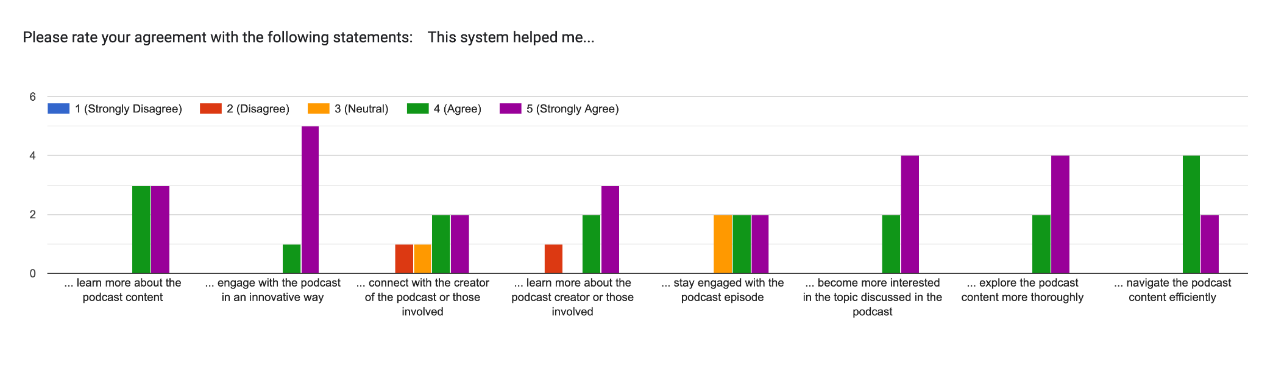
\includegraphics[width=1\textwidth]{figures/user1.png}
          \caption{User study survey results, rating agreement with "This system helped me..." prompts from 1 (Strongly Disagree) to 5 (Strongly Agree).}
        \end{figure}

        \begin{figure}[H]
        \centering
          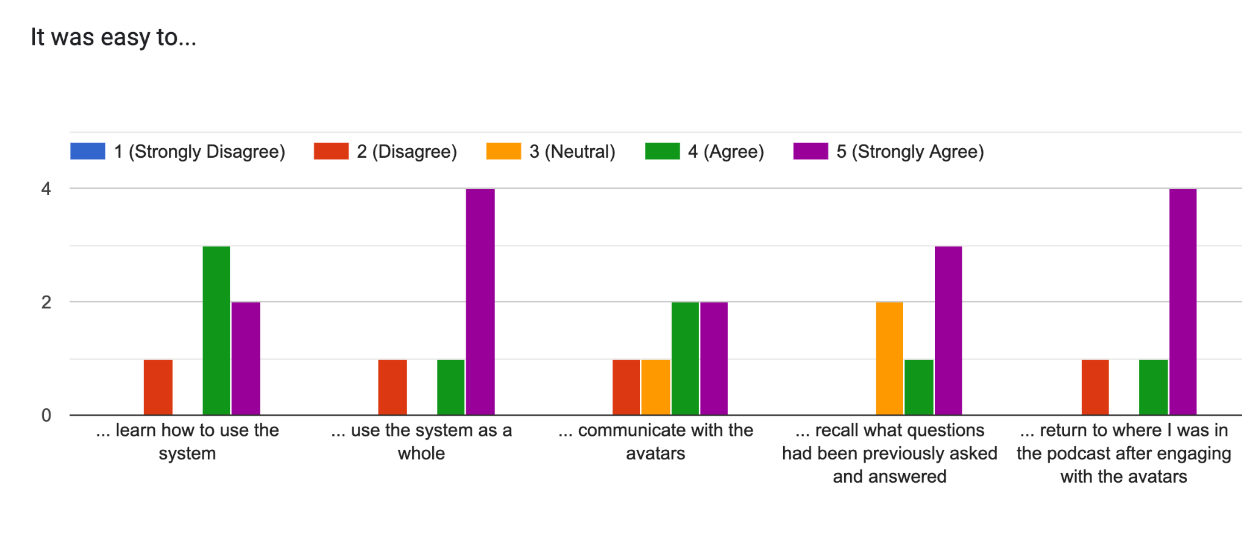
\includegraphics[width=1\textwidth]{figures/user2.png}
          \caption{User study survey results, rating agreement with "It was easy to..." prompts from 1 (Strongly Disagree) to 5 (Strongly Agree).}
        \end{figure}

        \begin{figure}[H]
        \centering
          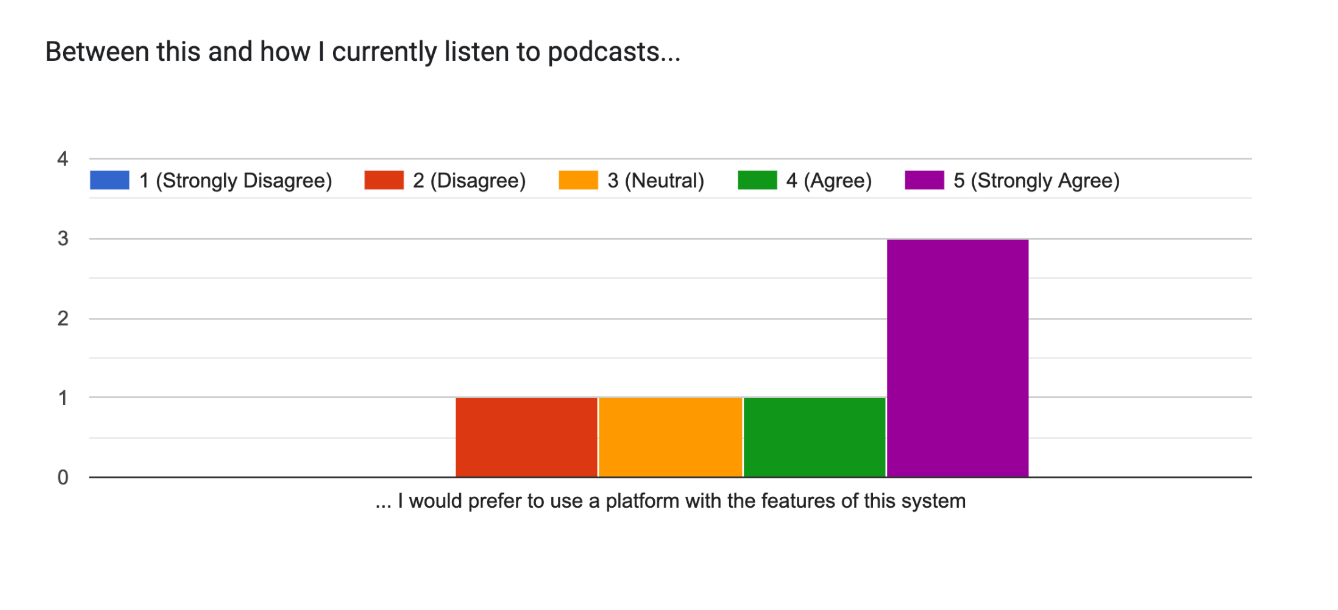
\includegraphics[width=1\textwidth]{figures/user3.png}
          \caption{User study survey results, rating agreement with "Between this and how I currently listen to podcasts..." prompts from 1 (Strongly Disagree) to 5 (Strongly Agree).}
        \end{figure}

        \begin{figure}[H]
        \centering
          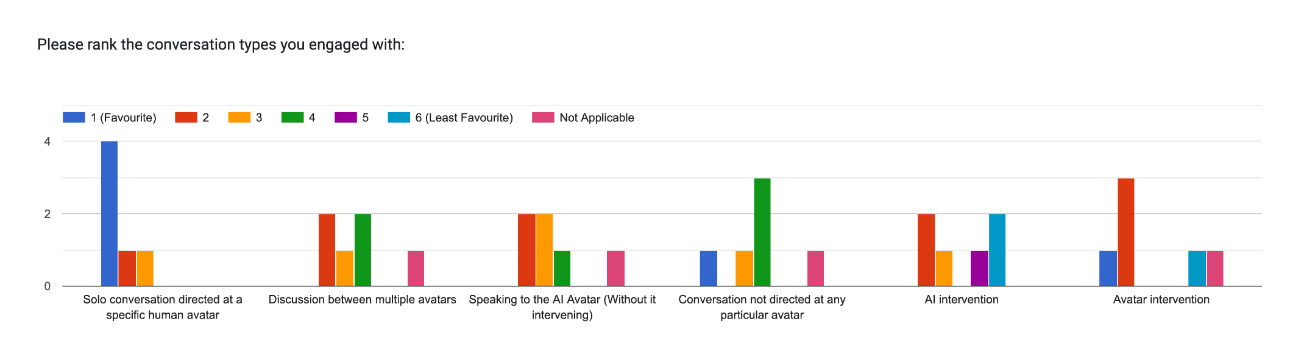
\includegraphics[width=1\textwidth]{figures/user4.png}
          \caption{User study survey results, ranking the different conversation types interacted with. one being the best, five being the worst.}
        \end{figure}

        \begin{figure}[H]
        \centering
          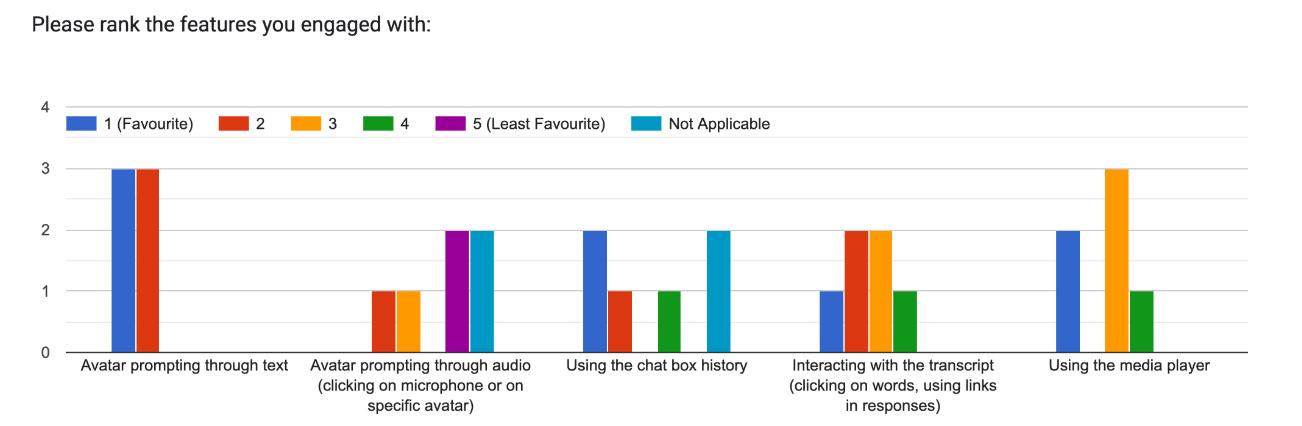
\includegraphics[width=1\textwidth]{figures/user5.png}
          \caption{User study survey results, ranking the specific features interacted with. one being the best, five being the worst.}
        \end{figure}
        
        \chapter{User Prompts \& System Responses}
        \label{app:K}
        The chat history from the final two user study sessions: \url{https://github.com/kierankasha/thesis/tree/main/chat%20history}. These files include user prompts, avatar responses, and transcript matches.
        
        \chapter{Consent Form}
        \label{app:L}
        This link contains the consent form used for both studies: \url{https://github.com/kierankasha/thesis/blob/main/supplementals/consent.pdf}.
        
    
    \end{myfont}
    \clearpage
    \blankpage
    \blankpage
\end{document}